%                                                                 aa.dem
% AA vers. 7.0, LaTeX class for Astronomy & Astrophysics
% demonstration file
%                                                 (c) Springer-Verlag HD
%                                                revised by EDP Sciences
%-----------------------------------------------------------------------
%
%\documentclass[referee]{aa} % for a referee version
%\documentclass[onecolumn]{aa} % for a paper on 1 column  
%\documentclass[longauth]{aa} % for the long lists of affiliations 
%\documentclass[rnote]{aa} % for the research notes
%\documentclass[traditabstract,letter,longauth]{aa} % for the letters 
%\documentclass[structabstract]{aa}  
%\documentclass[traditabstract]{aa} % for the abstract without structuration  % (traditional abstract)                                   
\documentclass[traditabstract]{aa}                                   
%
%\def\del#1{{\bf  [deleted text] }} \def\new#1{{\bf #1}} \def\remark#1{{\bf  [remark: #1]}}
\def\del#1{} \def\new#1{#1} \def\remark#1{}

\newcommand{\rmn}{\mathrm}
\newcommand{\CR}{\mathrm{CR}}
\newcommand{\expval}[1]{\left\langle #1 \right\rangle}
\newcommand{\RA}[3]{#1$^{\mathrm{h}}$#2$^{\mathrm{m}}$#3$^{\mathrm{s}}$}
\newcommand{\Dec}[3]{#1$^{\circ}$#2\arcmin#3\arcsec}
\newcommand{\dps}{\displaystyle}
\newcommand{\eps}{\varepsilon}

%
\usepackage{graphicx}
\usepackage{natbib}
%
\usepackage{txfonts}

\voffset0.5in

%%%%%%%%%%%%%%%%%%%%%%%%%%%%%%%%%%%%%%%%
\begin{document}

%%%%%%%%%%%%%%%%%%%%%%%%%%%%%%%%%%%%%%%%
\title{On the Physics of Radio Halos: Scaling Relations and Luminosity Function}

%%%%%%%%%%%%%%%%%%%%%%%%%%%%%%%%%%%%%%%%
\author{
 Fabio Zandanel\inst{1,*} \and
 Christoph Pfrommer\inst{2} \and
 Francisco Prada\inst{3,4,1}
}
\institute {Instituto de Astrof\'{\i}sica de Andaluc\'{\i}a (CSIC), Glorieta de la Astronom\'{\i}a, E-18080 Granada, Spain
 \and HITS, Schloss-Wolfsbrunnenweg 33, 69118 Heidelberg, Germany
 \and Campus of International Excellence UAM+CSIC, Cantoblanco, E-28049 Madrid, Spain
 \and Instituto de F\'{\i}sica Te\'orica, (UAM/CSIC), Universidad Aut\'onoma de Madrid, Cantoblanco, E-28049 Madrid, Spain
}

\date{Received XXX}

%%%%%%%%%%%%%%%%%%%%%%%%%%%%%%%%%%%%%%%
% \abstract{}{}{}{}{} 
% 5 {} token are mandatory
\abstract{
BLA BLA BLA
}

\keywords{galaxy cluster}

\titlerunning{On the Physics of Radio Halos: Scaling Relations and Luminosity Function}

\authorrunning{Zandanel et al.}

\maketitle


%%%%%%%%%%%%%%%%%%%%%%%%%%%%%%%%%%%%%%%%%%%%%%%%%%%%%%%%%%%%%%%%%%%
%%%%%%%%%%%%%%%%%%%%%%%%%%%%%%%%%%%%%%%%%%%%%%%%%%%%%%%%%%%%%%%%%%%
\section{Introduction}
\label{sec:1}
The presence of large scale diffuse synchrotron radio emission in clusters of galaxies proves the existence 
of relativistic electrons and magnetic fields permeating the intra-cluster medium (ICM) (see e.g.~\citealp{2004NewAR..48.1137F}).
\begingroup
\let\thefootnote\relax\footnotetext{ * fabio@iaa.es}
\endgroup
Diffuse cluster radio emission can be separated in two classes: radio relics and radio halos (see e.g.~\citealp{2004rcfg.procE..25K,2008SSRv..134...93F}). 
Radio (mini-)halos (RHs) are located at the center of clusters and are characterized by a regular and unpolarized morphology with clear
similarities with the thermal X-ray emission. On the contrary, radio relics typically lie at the cluster outskirts, have a irregular
morphology, and often show a high polarization. While relics seem to directly trace structure formation shocks (see e.g.~\citealp{2011A&A...533A..35V}), 
the explanation for the RHs phenomenon is challenging and still an open question.
                                   
Two principal models have been proposed to explain RHs.  In the ``hadronic model'' the radio emitting electrons are produced in cosmic ray (CR) proton-proton
interactions with the ICM, requiring only a very modest fraction of a few percent of CR-to-thermal pressure (see e.g.~\citealp{1997ApJ...477..560E, 
2001ApJ...559...59M,2003A&A...407L..73P, 2004A&A...413...17P, 2004MNRAS.352...76P, 2007IJMPA..22..681B, 2008MNRAS.385.1211P, 2008MNRAS.385.1242P, 2009JCAP...09..024K, 2010MNRAS.401...47D, 2010arXiv1003.0336D, 2010arXiv1003.1133K, 2010arXiv1011.0729K, 2011A&A...527A..99E}).  
CR protons and heavier nuclei, like electrons, can be accelerated and injected into the ICM by structure formation shocks, active 
galactic nuclei (AGN) and galactic winds.  Due to their higher masses with respect to electrons, CR protons are accelerated more efficiently to
relativistic energies and are expected to show a ratio of the spectral energy flux of CR protons-to-electrons above 1 GeV of about 100, similarly to
what is observed in our Galaxy \citep{2002cra..book.....S}. Additionally, CR protons have radiative cooling times larger than electrons by the square
of the mass ratio and therefore can accumulate in clusters for cosmological times \citep{1996SSRv...75..279V}. Indeed, CR electrons suffer more 
severe energy losses via synchrotron and inverse Compton emission at GeV energies, and Bremsstrahlung and Coulomb losses below 100~MeV.
In the ``re-acceleration model'', RHs are thought to be the result of electrons accelerated during powerful states of ICM turbulence, as a consequence of
a cluster merger (see e.g.~\citealp{1993ApJ...406..399G, 2002A&A...386..456G, 2005MNRAS.363.1173B, 2007MNRAS.378..245B,
2010arXiv1008.0184B, 2009A&A...507..661B}). This, however, requires a sufficiently long-lived CR electron 
population at energies around 100~MeV which might be maintained by re-acceleration at a rate faster than the cooling processes.  We refer the reader
to \citet{2011A&A...527A..99E} for a discussion on the strengths and weaknesses of these two models.

RHs themselves can be divided in two classes. Radio halos are typically associated with merging clusters and have very large extensions, e.g. the 
Coma cluster halo have an extension of about  2~Mpc. Radio mini-halos are associated with very relaxed clusters, that have a cool core
harboring the halo, and have typical extension of few hundred kpc, e.g. the Perseus cluster mini-halo has an extension of about 0.2~Mpc. 
The observed morphological similarities with the thermal X-ray emission suggests RHs may be of hadronic origin. Indeed, the hadronic model 
would naturally explain the RHs generation mechanisms and, moreover, directly predict the existence of radio halos and mini-halos depending 
on the cluster dynamical state. In fact, cool-core clusters (CCC) are characterized by very high thermal X-ray emissivity and very peaked ICM 
densities with respect to the merging non cool-core clusters (NCCC) (see e.g.~\citealp{2008A&A...487..431C}). This dramatic difference in 
the ICM density of CCC and NCCC would reflect in the two observed classes of RHs. 

The RHs luminosity seems strongly correlated also with the clusters thermal X-ray emissivity (see e.g.~\citealp{2009A&A...507..661B,2011A&A...527A..99E}).
However, a large fraction of clusters do not exhibit significant diffuse synchrotron emission of any kind. Galaxy clusters with the same thermal X-ray luminosity show
an apparent bimodality with respect to their radio luminosity. Either they harbor a RH or they do not have any detectable diffuse radio emission. 
This suggests the existence of a switch-on/switch-off mechanism able to change the radio luminosity by more than one order of magnitude.
While such a mechanism could be easily realized in the framework of the re-acceleration model \citep{2009A&A...507..661B}, the \emph{classical} 
hadronic model predicts the presence of RHs in all clusters. The failure to reproduce the observed cluster radio-to-X-ray bimodality was one of
the main criticisms against the hadronic model. Another criticism to the \emph{classical} hadronic model is the the fact that t does not reproduce 
some spectral features observed in clusters, as the total spectral curvature claimed in the Coma cluster radio halo or the spectral steepening observed at 
some RH edges. In a recent work, \cite{2011A&A...527A..99E} asses this problem by analyzing how the CR distribution is shaped within a cluster. While 
CR advection tends to result in centrally enhanced CR profiles, the propagation in form of CR streaming and diffusion tends to produce flat CR profiles. 
The different  effects of such CR transport phenomena may account, in the hadronic model, for the observed radio-to-X-ray bimodality, as shown by En{\ss}lin and 
collaborators, and can have an important impact in clusters in general. These phenomena were not considered in earlier analytical works (see 
e.g.~\citealp{2004A&A...413...17P,2004MNRAS.352...76P}) as well as in hydrodynamic simulations (see e.g.~\citealp{2008MNRAS.385.1211P,
2010MNRAS.409..449P}) for seek of simplicity, but can have indeed a dramatic impact.  We note that the effect of the CR transport processes 
may also explain the spectral features observed in some clusters (see \citealp{2011A&A...527A..99E} for details).

More recently, \cite{2012MNRAS.421L.112B} presented the first scaling relations between RH luminosity and Sunyaev-Zel'dovich (SZ) effect measurements,
using the \emph{Planck} cluster catalogue. He found that while the correlation agrees with previous scaling measurements based on X-ray data, there is no indication
for a bimodal cluster population divided into radio-loud and radio-quiet clusters.
 
A clear way out to disentangle between the hadronic and re-acceleration models is to search for the gamma-ray emission that results from
result of the neutral pion decays, secondary product of the hadronic CR interaction with the ICM, which is not predicted to be present
by the re-acceleration model. Such observational effort have been undertaken in the last few years (for space-based cluster observations in the GeV-band, 
see \citealt{2003ApJ...588..155R, 2010ApJ...717L..71A, 2010JCAP...05..025A,2012AAS...21920701Z,2012arXiv1201.1003H}; for ground-based 
observations in the energy band $>100$~GeV, see \citealt{2006ApJ...644..148P, 2008AIPC.1085..569P, 2009A&A...495...27A,2009arXiv0907.0727T, 
2009arXiv0907.3001D, 2009arXiv0907.5000G,cangaroo_clusters,2009ApJ...706L.275A,2010ApJ...710..634A,2011arXiv1111.5544M}) without being able to detect
cluster gamma-ray emission\footnote[1]{Recently \cite{2012arXiv1201.1003H} claimed an evidence for diffuse gamma-ray emission in the \emph{Fermi} satellite data of 
the Virgo cluster which however is excluded by a more recent analysis from the \emph{Fermi} collaboration itself (see Elliot Bloom talk at the UCLA Dark Matter 2012 conference, https://hepconf.physics.ucla.edu/dm12/).}.
Despite the negative detections, we have been starting to put significant constraints on the gamma-ray predictions. The long observation campaign of the Perseus 
galaxy cluster performed by the Major Atmospheric Gamma-ray Cherenkov (MAGIC) telescopes constrains the cluster average CR-to-thermal pressure to 
be less than few percents \citep{2010ApJ...710..634A,2011arXiv1111.5544M}. Comparing the corresponding upper limits to predictions from 
simulations of \cite{2010MNRAS.409..449P} constrains the maximum CR acceleration efficiency at structure formation shocks to be $<50\%$. 
Alternatively, this may indeed suggest the presence of non-negligible CR transport processes into the outer cluster regions as explored by \cite{2011A&A...527A..99E}. 
Constraints at the same level are confirmed also by the \emph{Fermi}-Large Area Telescope (LAT) data on the Coma cluster \citep{2012AAS...21920701Z,2012arXiv1201.1003H}. This however does not allow us to make any definitive statement on the RHs generation mechanisms as the hadronic model is still far from being really 
probed by gamma-ray observations.

An important step forward in this scenario would come from detailed RHs population analyses. Actually, we know only about 30 clusters that harbor RHs (see 
\citealp{2011A&A...527A..99E} for an almost up-to-date list) and only two X-ray flux-limited studies, relevant for the universally of the conclusions, 
have been made out of which only few clusters resulted to host a RH  \citep{1999NewA....4..141G,VenturiGMRT_2}. With such small samples, the
conclusions than can be drown on the underlying mechanisms acting in the RHs generation are not very robust. Fortunately, this is going to change thanks to 
the next-generation radio observatory Low Frequency Array (LOFAR) which officially started operations in 2010.\footnote[2]{www.lofar.org}
In fact, a deep cluster survey is part of the LOFAR science key projects. This will soon provide us with a large number of radio-observed galaxy clusters 
up to redshift $z\approx1$ (see e.g.~\citealp{2010A&A...509A..68C,2012JApA..tmp...34R}).
This would hopefully permit to clearly determine the RHs characteristics against the galaxy cluster properties investigating the relations between 
radio-loud/quiet, non cool-core/cool-core and non-merging/merging clusters, and exploring the role of different parameters like the magnetic field, 
the CR acceleration efficiency, and the CR transport properties.

In this work, we present predictions for the RHs of a complete cosmological sample of galaxy clusters up to redshift 1, obtained from the MultiDark N-body 
cosmological simulation \citep{2011arXiv1104.5130P}. We construct a \emph{phenomenological} model to assign to each halo in the MultiDark simulation 
a gas density profile such as it reproduce the basic observed X-ray cluster properties. We assume that the RHs are generated by secondaries of the hadronic 
CR interactions with the ICM. In adopting the hadronic scenario, we construct a \emph{hybrid} model merging the result of hydrodynamic simulations by \cite{2010MNRAS.409..449P} and the analytical model by \cite{2011A&A...527A..99E}.  As anticipated above, the inclusion of the latter is particularly important as CR transport 
processes have a dramatic impact on overall emission shape and normalization. In fact, thanks to this, we are able to reproduce the main RHs characteristics and both
the radio-to-X-ray and radio-to-SZ scaling relations. We show, once again, that the hadronic model is a perfectly viable explanation for RHs and it is not in tension 
with any of current observations or constraints. We obtain RHs luminosity functions at different redshifts, and present predictions for the LOFAR
cluster survey. 

%%%%Paper Summary
In Section~\ref{sec:2}, we explain the methodology adopted to obtain from N-body, so dark matter (DM) only, simulated clusters the corresponding ICM gas densities.
In doing this, we check that  our approach is able to reproduce the main observed cluster X-ray properties. We then construct the model for CR distribution 
in clusters. In Section~\ref{sec:4}, we apply it to some RHs in order to show how it works and adapts to different situations. We investigate the radio-to-X-ray and radio-to-SZ scaling relations and the radio luminosity function of our simulated sample with respect to current observations in Section~\ref{sec:4}. We produce RHs luminosity functions at different redshifts and discuss them in view of the LOFAR cluster survey in Section~\ref{sec:5}. Finally, in Section~\ref{sec:6}, we present our conclusions.
%%%%Constants
In this work, the cluster mass $M_{x}$ and radius $R_{x}$ are defined with respect to $x=200$ or $x=500$ times the Universe \emph{critical} density. We adopt $\Omega_{\rm{m}}=0.3$, $\Omega_{\rm{\Delta}}=0.7$ and $H_0 = 100 \times h_{70}$~km~s$^{-1}$~Mpc$^{-1}$ where $h_{70} = 0.7$. 


%%%%%%%%%%%%%%%%%%%%%%%%%%%%%%%%%%%%%%%%%%%%%%%%%%%%%%%%%%%%%%%%%%%
%%%%%%%%%%%%%%%%%%%%%%%%%%%%%%%%%%%%%%%%%%%%%%%%%%%%%%%%%%%%%%%%%%%
\section{Methodology}
\label{sec:2}
The two fundamental ingredients of this work are the cosmological simulation of the Universe from which we construct our complete cluster 
sample, and the emission model. We use here the MultiDark simulation which characteristics, along with our final cluster sample, 
are described in the next Section~\ref{sec:2.1}. 
%
As we will see, for any given cluster, the necessary ingredients for the emission model are mass, temperature, and gas density 
distribution. We construct a complete cluster sample from an N-body cosmological simulation, i.e. a \emph{DM-only} 
simulation, where we assign to each object a gas density profile phenomenologically constructed from state-of-art 
X-ray observations, as shown in Section~\ref{sec:2.2}. In doing this, we show that the approach can reproduce the known 
X-ray cluster characteristics, as the $L- M$ and $Y_{\rm{X}}-M$ relations, the X-ray luminosity function (XLF), and the $Y_{\rm{SZ}}-M$ relation. 
The underlying idea is that if we can reproduce the X-ray observations, we can safely adopt our gas density profiles to predict the radio 
and gamma-ray emission. 
%
The model used to calculate the radio, as well as the gamma-ray, emission will be then constructed in Section~\ref{sec:2.3}.

%%%%%%%%%%%%%%%%%%%%%%
\subsection{MultiDark Simulation and Final Cluster Sample}
\label{sec:2.1}
The MultiDark simulation\footnote[3]{www.multidark.org} used in this work is described in 
detail in \cite{2011arXiv1104.5130P} and \cite{2011arXiv1109.0003R}.  It is a N-body cosmological simulation 
done with the the Adaptive-Refinement-Tree (ART) code \citep{1997ApJS..111...73K} of $2048^3$ particles within
a ($1000$~Mpc~h$^{-1}$)$^3$ cube. The latest WMAP5 and WMAP7 cosmological parameters 
were used. This simulation is particularly  well suited for our purpose because of its large number clusters. 
 
We use the MultiDark halo catalog, constructed with the Bound Density Maxima algorithm \citep{1997astro.ph.12217K}.
We will mainly use $M_{500}$ and $R_{500}$ for comparison with existing observational works. 
We use the technique described in \cite{2003ApJ...584..702H} to convert $M_{200}$ and $R_{200}$ provided by the BDMW halo catalog to $M_{500}$ and $R_{500}$.
In creating our cluster sample we only select distinct halos, i.e. those halos that are not the sub-halos
of any other halo. This is because we are going to use cluster global properties and therefore we cannot
deal with substructures.

Additionally, we assume that the main emission mechanism in the ICM is the thermal bremsstrahlung, which is true only above approximately $3\times10^{7}$~$\rmn{K}\approx2.6$~keV \citep{1988xrec.book.....S}. Below this temperature there could be other important emission contributes, from e.g. emission lines, with which we do not want to treat for simplicity. Therefore, we impose a cut mass cut of $M_{200}\geq1\times10^{14}$~$h^{-1}$~M$_{\odot}\approx1.4\times10^{14}$~$h_{70}^{-1}$~M$_{\odot}$ which ensures us temperatures above approximately 2.6~keV assuming the $M_{500} - T_{\rm{ci}}$ relation found in \cite{2010MNRAS.406.1773M}.

Finally, the LOFAR radio observatory is expected to detect RHs up to redshift $z \approx 1$. Therefore, for our predictions, we make use of different simulation snapshots up
to $z=1$. In Table~\ref{tab:z}, we resume the total number of objects in our final cluster sample at different redshifts.

\begin{table}[hbt!]
\begin{center}
\caption{Number of Halos in the Final Cluster Sample}
\medskip
\begin{tabular}{cc}
\hline
\phantom{\Big|}
Redshift $z$ & Number of Halos \\
\hline\\[-0.5em]
 0 &  13763\\
 0.2 &  12398\\
 0.3 &  10783\\ 
 0.4 &   7789\\ 
 0.61 &  5187\\ 
 0.78 &  3372\\ 
 1 &  1803\\[0.5em]
\hline
\end{tabular}
\label{tab:z}
\end{center}
\footnotesize{Note. Number of halos in our MultiDark snapshots at redshift $z$ for $M_{200}\geq1\times10^{14}$~$h^{-1}$~M$_{\odot}\approx1.4\times10^{14}$~$h_{70}^{-1}$~M$_{\odot}$. }
\end{table}


%%%%%%%%%%%%%%%%%%%%%%%%%%%%%%%%%%%%%%%%%%%%%%%%%%%%%%%%%%%%%%%%%%%
\subsection{Gas Density Modeling and X-ray Observables}
\label{sec:2.2}
We will show in next Section~\ref{sec:2.3} that our emission model needs the ICM gas density profile as an input.
Our cluster sample is based on an N-body cosmological simulation; obviously we do not have the information for the baryonic component.

We decided to use a \emph{phenomenological} approach and to construct the gas density profiles directly from sate-of-art X-ray observations.
The best X-ray observations, with the available information needed for our purposes, are given by the representative \emph{XMM-Newton} cluster structure survey (REXCESS) sample \citep{2008A&A...487..431C,2009A&A...498..361P}. It is a sample of 31 galaxy cluster of different dynamical states at redshift $0.06<z<0.18$ with detailed informations of the de-projected electron density profiles \citep{2008A&A...487..431C}. The REXCESS gas profiles represented an important step forward with respect to the commonly used $\beta$ and double-$\beta$ profiles of elder works, as the HIFLUGCS cluster sample \citep{2002ApJ...567..716R}. In Figure~\ref{fig:gas_profiles}, we show the 31 electron density profiles of the REXCESS sample color-coded in cool-core and non-cool-core clusters (hereafter CCC and NCCC, respectively).

\begin{figure}[hbt!]
\centering
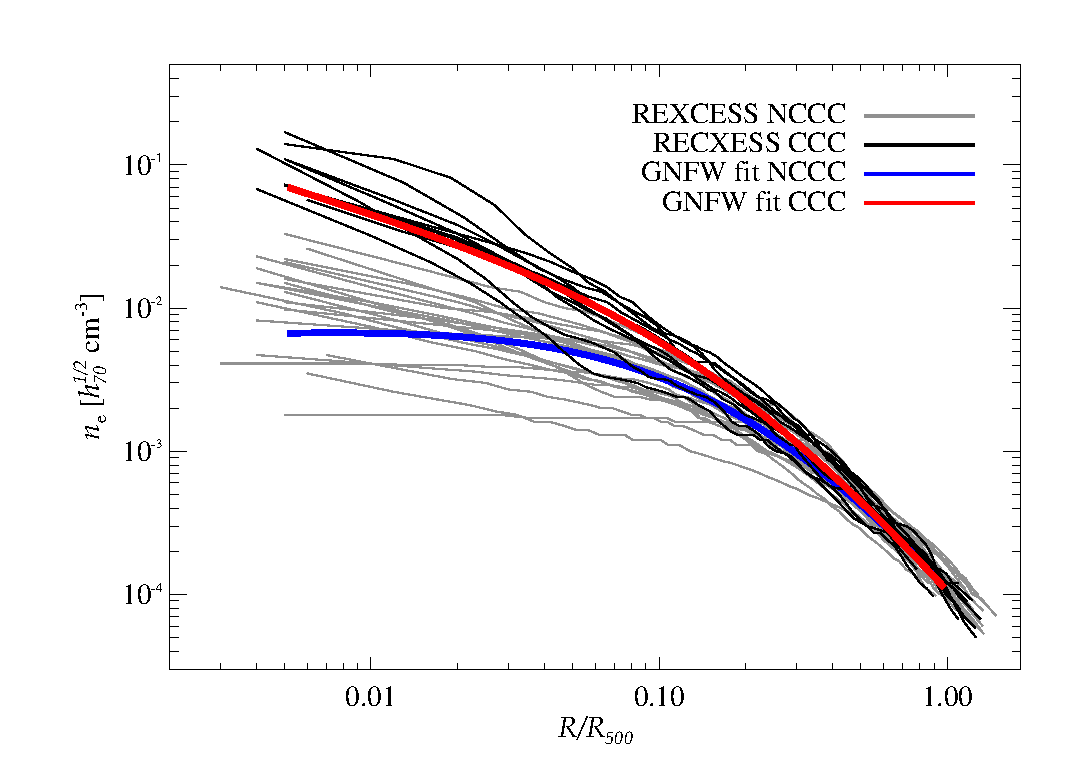
\includegraphics[width=0.5\textwidth]{figures/gas_profiles.eps}
\caption{Electron density profiles of the 31 clusters in the REXCESS sample. Grey and black lines represent NCCC and CCC clusters, respectively. The blue and red lines represent our GNFW mean profile for the NCCC and CCC clusters, respectively.}
\label{fig:gas_profiles}
\end{figure}

In order to obtain a general electron density profile to be \emph{plugged} onto our simulated clusters, we use a generalized Navarro-Frank-White (GNFW) profile:

\begin{equation}
n_{\rm{e}}(x) = \frac{n_{0}}{x^{\beta}\left[1+x^{\alpha}\right]^{\frac{\delta-\beta}{\alpha}}}
\label{eq:gnfw}
\end{equation}

where $x=R/R_{\rm{c}}$ and $R_{\rm{c}}$ is the cluster core radius. For simplicity we fix $R_{\rm{c}} = 0.2 \times R_{500}$, $\alpha = 1$ and $\delta = 2.5$ as good values representing the whole sample. We then fit in log-log space the REXCESS profiles separating them in the two categories of NCCC and CCC as shown in grey and black, respectively, in Figure~\ref{fig:gas_profiles}. The resulting fits are shown in blue and red for the NCCC and CCC population, respectively. We obtain $n_{\rm{0,NCCC}} = 1.02\times10^{-2}$~$h_{70}^{1/2}$~cm$^{-3}$, $n_{\rm{0,CCC}} = 8.32\times10^{-3}$~$h_{70}^{1/2}$~cm$^{-3}$, $\beta_{\rm{NCCC}} = -0.093$ and $\beta_{\rm{CCC}} = 0.592$.

The next step is to introduce a mass-scaling in order to apply our GNFW profiles to all our clusters. We adopt $f_{gas,500}-M_{500}$ relation of \cite{2009ApJ...693.1142S} (their Equation~(8)). We can express $f_{\rm{gas},500}$ in the following way:

\begin{equation}
f_{\rm{gas},500} = \frac{M_{\rm{gas},500}}{M_{500}}  = \frac{\int_{0}^{R_{500}} \rho_{\rm{gas}} \rmn{d}V}{M_{500}}
\label{eq:m500}
\end{equation}

with $\rho_{\rm{gas}} = n_{\rm{e}} m_{\rm{p}} / ( X_{\rm{H}}X_{\rm{e}} )$ where $m_{\rm{p}}$ is the proton mass, $X_{\rm{H}} = 0.76$ is the primordial hydrogen mass fraction and $X_{\rm{e}} = 1.157$ the ratio of electron-hydrogen number densities in the fully ionized ICM \citep{1988xrec.book.....S}. For each cluster $i$ of our sample, we then define a new \emph{mass-scaled} gas profile as $\rho_{\rm{gas},i}=C_{i} \times \rho_{\rm{gas}}$ with:

\begin{eqnarray}
%C_{i}  =  (0.0616\pm(0.0060g_{1}))  h_{73}^{-1.5}  \left(\frac{M_{500,i}}{10^{13} h_{73}^{-1} \rmn{M_{\odot}}}\right)^{0.135\pm(0.030g_{2})} \nonumber \\
C_{i}  & = &  (0.0656\pm(0.0064g_{1}))  h_{70}^{-1.5}  \nonumber \\
 & \times & \left(\frac{M_{500,i}}{1.04 \times 10^{13} h_{70}^{-1} \rmn{M_{\odot}}}\right)^{0.135\pm(0.030g_{2})} \frac{M_{500,i}}{\int_{0}^{R_{500,i}} \rho_{\rm{gas}} \rmn{d}V}
\label{eq:gas_scaling}
\end{eqnarray}
 
where $g_{1}$ and $g_{2}$ are random Gaussian number which we use in order to simulate the natural scatter of the gas profiles.\footnote[4]{The values $0.0064$ and $0.03$ quoted in Equation~(\ref{eq:gas_scaling}) do not represent the proper scatter of the $f_{\rm{gas},500}-M_{500}$ relation but just the parameter errors.} 

In this way, for each cluster in our sample we obtain a gas density profile $\rho_{\rm{gas},i}$ uniquely determined by its DM mass $M_{500,i}$ and by the property of being NCCC or CCC. This latter property is assigned considering the merging history of our halos. In particular, we make use of the offset parameter $X_{\rm{off}}$ taken from the MultiDark BDMW catalog. This is defined as the ratio between the difference of the distance from the halo center to the center of mass and the virial radius. The parameter assesses the dynamical state of the cluster and tell us if the halo has suffered a recent merger or not. Current observations reveal a NCCC/CCC proportion of about $50/50\%$ (see e.g.~\citealp{2007A&A...466..805C,2009MNRAS.395..764S}).  {\bf Motivate the following choice.} Our approach is therefore to use the median of the $X_{\rm{off}}$ distribution of our sample and define the halos below this value as non-merging CCC and the ones above this value as merging NCCC.

The final ingredient for our gas profiles is the redshift evolution. We decided to include it because we want to compare our results with observations at different redshifts up to $z=1$. The two generalized NCCC and CCC gas profiles are virtually not dependent on the REXCESS clusters redshift itself because we are obtaining just the two profile shapes from it and we scale them to different masses with the $f_{\rm{gas},500}-M_{500}$ relation of \cite{2009ApJ...693.1142S}. The 43 clusters used in \cite{2009ApJ...693.1142S} have redshifts $0.012 < z < 0.12$ with a \emph{median} of $z \approx 0.04$, therefore we consider our final gas profiles correctly derived for the $z = 0$ simulation snapshot. For the higher redshifts catalogs given in Table~\ref{tab:z}, we include a \emph{self-similar} scaling $E(z)^{2} = \Omega_{\rm{m}} (1+z)^{3} + \Omega_{rm{\Delta}}$ in the gas density as $\rho_{\rm{gas}}(z) = E(z)^{2} \rho_{\rm{gas}}(z=0)$.

In order to check whether our phenomenological derived gas profiles are actually reproducing the observations, we calculate the bolometric X-ray thermal bremsstrahlung luminosity $L_{\rm{bol}}$ as in \cite{1988xrec.book.....S}\footnote[5]{We check our procedure fitting individually each of the 31 REXCESS clusters with the Equation~(\ref{eq:gnfw}) and calculating $L_{\rm{bol}}$ using their own gas temperature. We under-produce their observed luminosity by a mean (median) of about $21\%$ ($20\%$) which is reasonable considering that we do not permit the parameters $R_{\rm{c}}$, $\alpha$ and $\gamma$ to vary between different objects. Additionally, we do not consider other processes as e.g. emission lines which may give an important contribute particularly in the cluster outskirts.} and compare our sample result with the observed $L_{\rm{bol}} - M_{500}$ relation and XLF\footnote[6]{The mean (median) difference at $z=0$ between calculating $L_{\rm{bol}}$ up to $R_{200}$ or to $R_{500}$ is $\approx 5\%$ ($\approx 7\%$), with respect to $R_{200}$, therefore it is negligible. However, for consistency, in the following $L_{\rm{bol}}$ will refer to the quantity calculated within $R_{500}$.}. 

The missing parameter needed to calculate $L_{\rm{bol}}$ is the cluster temperature. We adopt the results obtained in \cite{2010MNRAS.406.1773M}:

\begin{equation}
\log_{10} \left( \frac{k_{\rm{B}}T_{\rm{ci}}}{\rm{keV}} \right) = A + B~\log_{10} \left( \frac{E(z) M_{500}}{10^{15} h_{70}^{-1} \rm{M_{\odot}}} \right)
\label{eq:temp}
\end{equation}
 
where $A=0.91$, $B=0.46$, $T_{\rm{ci}}$ is the cluster temperature \emph{not} centrally excised (see \citealp{2010MNRAS.406.1773M}) and $k_{\rm{B}}$ is the Boltzmann constant. As \cite{2010MNRAS.406.1773M} reports the scatter of this relation, which is $\sigma_{\rm{yx}} = 0.06,$\footnote[7]{Scatter is calculated as $\sigma_{\rm{yx}} = \sqrt{ ( \Sigma_{i=1}^{N} (Y_{i}-(A+B~X_{i}))^{2}) ) / N-1}$ where the sum is over the data points $X_{i}, Y_{i}$, and $A$ and $B$ are the fit parameters.}, we apply it to our sample, using a Gaussian random number, when calculating the cluster temperature. 

In Figure~\ref{fig:X_LM} left panel, we show how our predictions for the $L_{\rm{bol}}-M_{500}$ relation compare with the current observations. We can reproduce remarkably well the \cite{2010MNRAS.406.1773M} result (\emph{all} data, see their Table~7). Their sample is composed of clusters at $0.02<z<0.46$ with a median of $z \approx 0.2$. For this reason, we compare the \cite{2010MNRAS.406.1773M} result to our $z=0.2$ sample, and we limit the comparison in the mass range covered by the observations.
In Table~\ref{tab:LMfits}, we report our prediction for the $L_{\rm{bol}}-M_{500}$ scaling relation at different redshifts along with its scatter. We find that the scatter of our samples at different redshifts are in all cases distributed as a Gaussian with $\sigma_{yx} \approx 0.18$ correctly reproducing observations of \cite{2010MNRAS.406.1773M} which report a scatter of $\sigma_{yx} = 0.185$.

\begin{figure*}[hbt!]
\centering
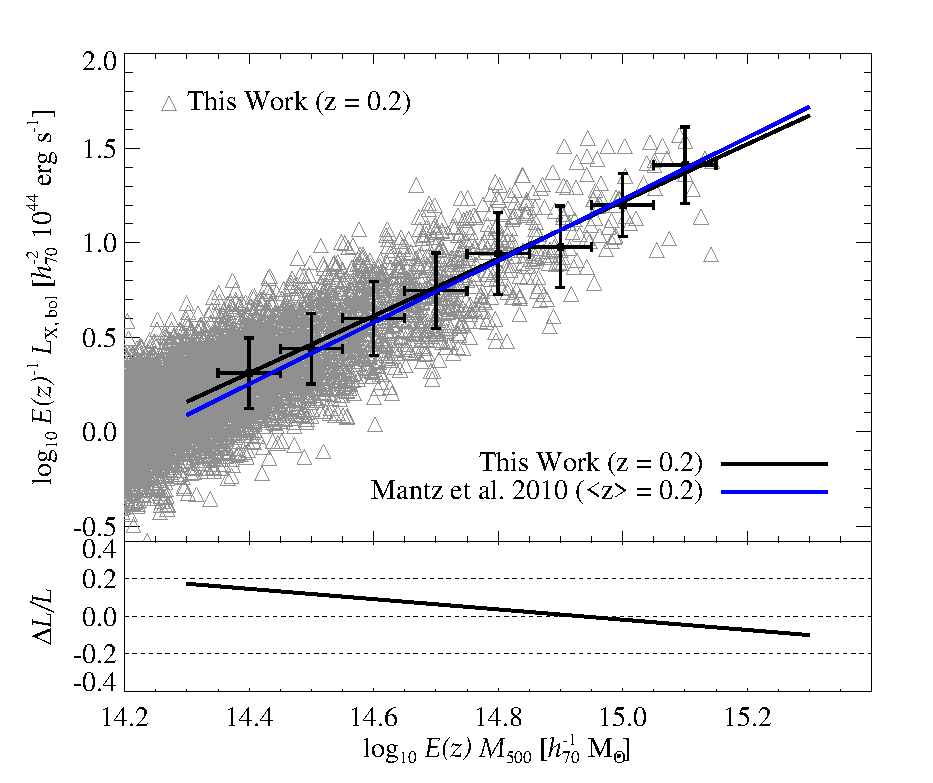
\includegraphics[width=0.33\textwidth]{figures/lx_m.eps}
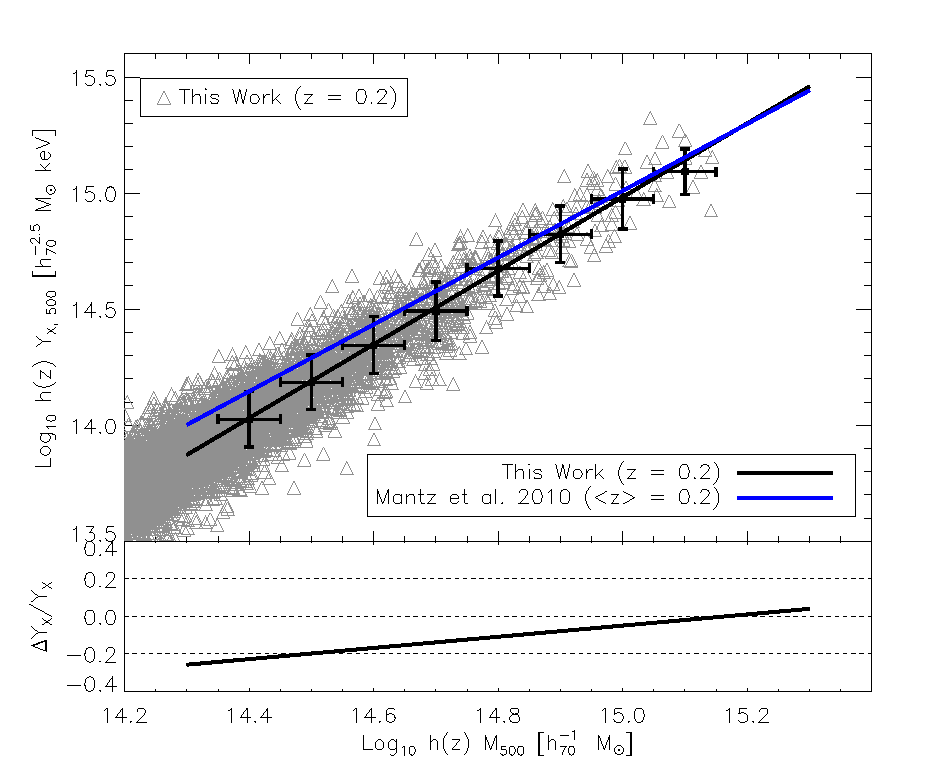
\includegraphics[width=0.33\textwidth]{figures/yx_m.eps}
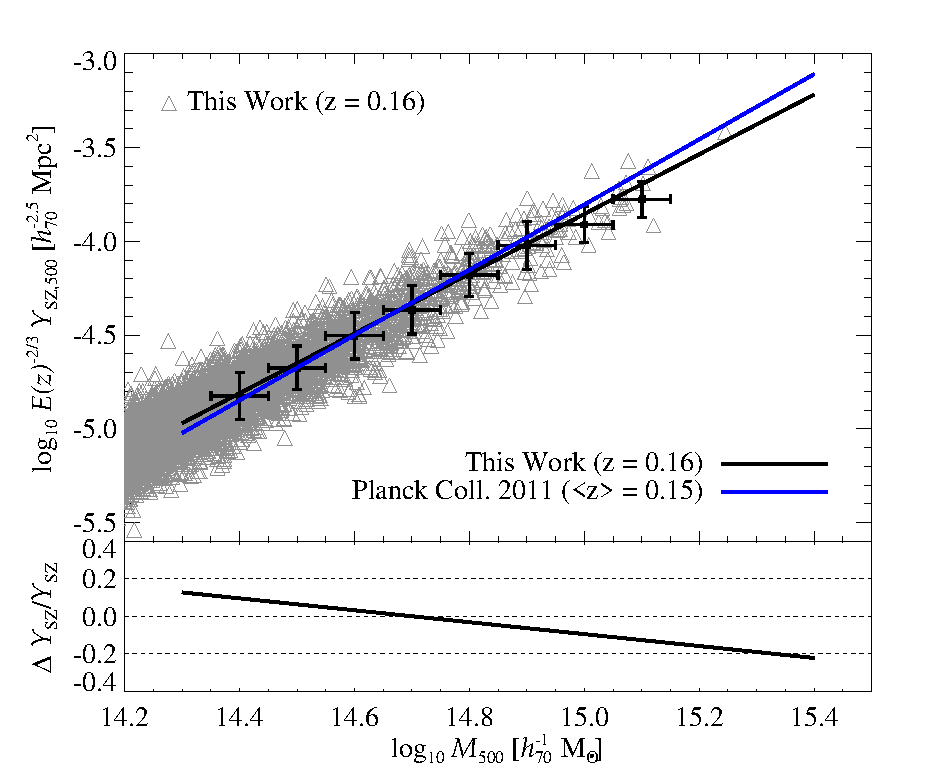
\includegraphics[width=0.33\textwidth]{figures/sz_m.eps}
\caption{X-ray and SZ scaling relations. \emph{Left.} X-ray thermal bremsstrahlung luminosity--to--mass relation. Grey triangles show the $z=0.2$ sample built from the MultiDark simulation and the black line is the corresponding scaling relation. The blue line is the experimental result obtained by \cite{2010MNRAS.406.1773M} with a sample of clusters with a median of $z \approx 0.2$. \emph{Center.} $Y_{\rm{X}}$--to --mass scaling relation. Grey triangles show the $z=0.2$ MultiDark sample and the black line is the corresponding scaling relation. The blue line is the experimental result obtained by \cite{2010MNRAS.406.1773M}. \emph{Right.} Sunyaev-Zel'dovich $Y_{\rm{SZ}}$--to-- mass scaling relation. Grey triangles show both the $z=0.1$ and the $z=0.2$ samples and the black solid and dashed lines are the corresponding scaling relations. The blue line is the result obtained by \cite{2011A&A...536A..11P} with a median redshift of about $0.15$. In all the plots, we limit the comparison in the mass range covered by observations. The bottom panels shows the difference of this work (calc) with respect to observations (obs) as $\Delta Y/Y = (Y_{\rm{fit,calc}}-Y_{\rm{fit,obs}})/Y_{\rm{fit,obs}}$. Additionally shown in black are the $Y$ medians of our halos in mass bins (horizontal error bars), where the vertical error bars represent the bin standard deviation. Note that, for $Y_{\rm{SZ}}$, in calculating the median we considered together the $z=0.1$ and $z=0.2$ samples which may result in a bias of the medians toward the more populated $z=0.1$ sample. This is true also for the highest-mass median point which contains few objects, all belonging to the $z=0.1$ sample.}
\label{fig:X_LM}
\end{figure*}

\begin{table}[hbt!]
\begin{center}
\caption{$L_{\rm{bol}}-M_{500}$ Scaling Relations.}
\medskip
\begin{tabular}{cccc}
\hline
\phantom{\Big|}
Redshift $z$ & $A$ & $B$ & $\sigma_{yx}$ \\
\hline \\[-0.5em]
 0      & $-21.41\pm0.11$ & $1.50\pm0.01$ & 0.179\\
 0.1   & $-21.30\pm0.12$ & $1.50\pm0.01$ & 0.179\\
 0.2   & $-21.50\pm0.13$ & $1.51\pm0.01$ & 0.178\\ 
 0.4   & $-21.13\pm0.17$ & $1.49\pm0.01$ & 0.178\\ 
 0.61 & $-21.59\pm0.22$ & $1.53\pm0.01$ & 0.177\\ 
 0.78 & $-20.73\pm0.29$ & $1.48\pm0.02$ & 0.177\\ 
 1      & $-20.45\pm0.42$ & $1.46\pm0.03$ & 0.177\\[0.5em]
\hline
\end{tabular}
\label{tab:LMfits}
\end{center}
\footnotesize{Note. Scaling relations are reported in the form of $\log_{10}~(L_{\rm{bol}}~/~E(z)~h_{70}^{-2}~10^{44}~\rmn{erg~s}^{-1})=A+B~\log_{10}~(E(z)~M_{500}~/~h_{70}^{-1}~\rmn{M_{\odot}})$. The relation scatter $\sigma_{yx}$ is also shown.
}
\end{table}

In comparing with observations, we take as reference \cite{2010MNRAS.406.1773M}. There are however many other works on this scaling relation, in particularly we recall the HIghest X-ray FLUx Galaxy Cluster Sample (HIFLUGCS; \citealp{2002ApJ...567..716R}), the REXCESS \citep{2009A&A...498..361P} sample, and the 115 \emph{Chandra} cluster sample of \cite{2007ApJ...668..772M}. The results on the slopes of the $L-M$ relation can vary significantly between different samples. While the slope of \cite{2010MNRAS.406.1773M} is $1.63\pm0.06$, \cite{2002ApJ...567..716R}\footnote[8]{Note that we are quoting the $L_{\rm{bol}}-M_{200}$ results of \cite{2002ApJ...567..716R}.} found values between $1.72\pm0.09$ and $1.89\pm0.08$ (depending on the fit procedure, which also can affect the final result), \cite{2009A&A...498..361P} found $2.08\pm0.13$ and \cite{2007ApJ...668..772M} found $1.96\pm0.10$. Discrepancies can come from many different sources but likely are to be charged to the selection criteria of the different samples as recently pointed out also by \cite{2011arXiv1109.3708R}. Samples which differ in e.g.~redshift distribution, mass range, fitting procedure and biases treatment, and, of course, the used instrument, can give and actually gave different results. Therefore we decided to take as reference the \cite{2010MNRAS.406.1773M} work because it is very recent, their sample is composed by a high number (238) of objects, and, more importantly, their analysis takes self-consistently into account all selection effects, covariances, systematic uncertainties and the cluster mass function (see also \citealp{2010MNRAS.406.1759M}).

The XLF study has been somehow abandoned during the last years due to the difficulties of using the X-ray luminosity for cosmological purposes. This is principally due to the square dependence of $L_{\rm{bol}}$ with $\rho_{\rm{gas}}$ which significantly varies from cluster to cluster in a way that we do not fully understand. We want however to see how the XLF looks like for our sample and take as reference the \emph{ROSAT} brightest cluster sample (BCS) XLF \citep{1997ApJ...479L.101E}, which is well in agreement with results from the ROSAT ESO Flux-Limited X-ray (REFLEX; \citealp{2002ApJ...566...93B}) and HIFLUGCS \citep{2002ApJ...567..716R} samples. Note that the XLF is fully determined by the clusters mass function and the $L-M$ relation once all the biases, and the scatter, are taken into account. This means that applying the \cite{2010MNRAS.406.1773M} $L-M$ relation directly to the MultiDark simulation mass function, the obtained XLF is exact assuming the \cite{2010MNRAS.406.1773M} result is correct.
In Figure~\ref{fig:XLF}, we show the \cite{2010MNRAS.406.1773M} XLF in the $0.1-2.4$~keV and bolometric bands, the BCS $0.1-2.4$~keV data points, $0.1-2.4$~keV and bolometric Schechter fits, and finally the bolometric prediction of our model. The $0.1-2.4$~keV \cite{2010MNRAS.406.1773M} XLF is well in agreement with the BCS data points but deviates from the corresponding Schechter fit at low luminosities. This is true also in the bolometric band, for which the BCS data points are not available, where the \cite{2010MNRAS.406.1773M} XLF and our prediction, which well agrees between themselves, deviate from the BCS Schechter fit at low luminosities. This may be an artifact due to the use of Schechter fit instead of the data points or may point to a low luminosity incompleteness of the BCS sample. Note that the Poissonian errors of the XLF obtained from the MultiDark simulation are somehow underestimated as using just one simulation realization we are not considering the uncertainty coming from the cosmic variance. The XLF study is becoming again a hot topic with the incoming launch of the eROSITA satellite (see e.g.~\citealp{2011MSAIS..17..159C}) and further studies in this direction are desirable. For these reasons, we do not show XLF predictions at other redshifts, leaving this for a future study (Zandanel et al., in prep.). 

\begin{figure}[hbt!]
\centering
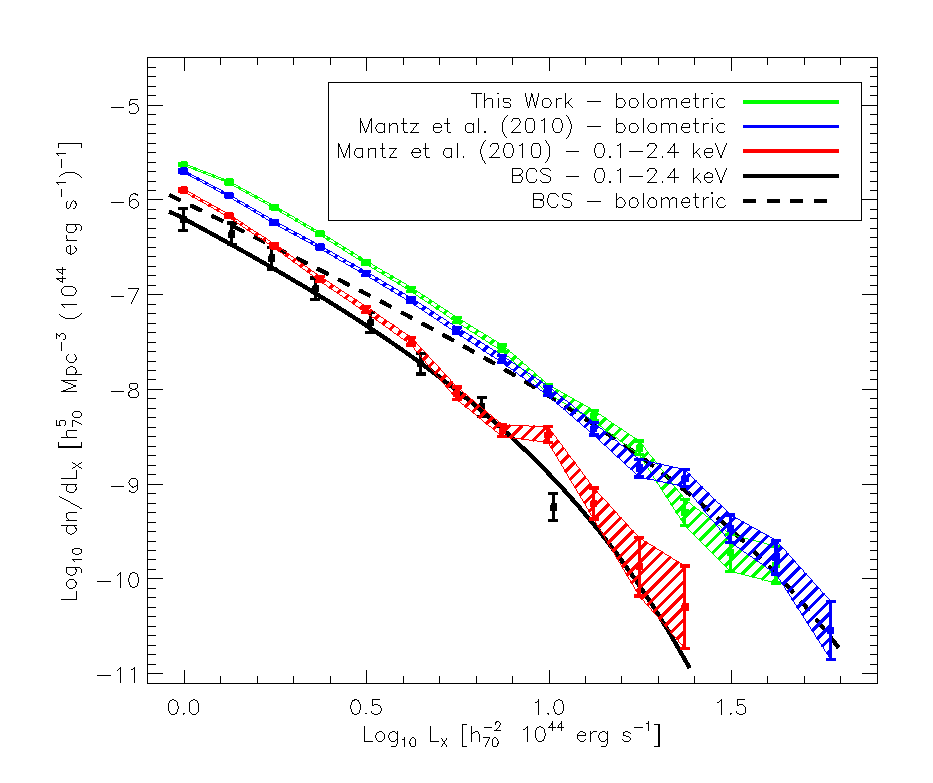
\includegraphics[width=0.48\textwidth]{figures/xlf.eps}
\caption{Bolometric X-ray luminosity function. Shown are the $0.1-2.4$~keV data points, the $0.1-2.4$~keV and bolometric Schechter fits of the BCS sample from \cite{1997ApJ...479L.101E}. The BCS sample is composed by clusters at $z\leq0.3$ with a median of $z \approx 0.08$. We therefore compare it to our MultiDark $z=0.1$ snapshot. We show the \cite{2010MNRAS.406.1773M} $0.1-2.4$~keV result which well compares with the BCS data points but deviate from the corresponding Schechter fit. We finally show the \cite{2010MNRAS.406.1773M} bolometric result and the bolometric prediction of our model. The XLFs are calculated in equally log-spaced mass bins; the reported error bars represent the Poissonian errors. Note that we limit the comparison in the luminosity range covered by our sample, where we cut the lowest part because in that range the XLF rapidly drops due to the imposed mass cut.
}
\label{fig:XLF}
\end{figure}

There are other two extremely important quantities in cluster studies, and in their cosmological applications. These are the $Y_{\rm{X}}$ parameter \citep{2006ApJ...650..128K} and the Sunyaev-Zel'dovich $Y_{\rm{SZ}}$ parameter (see e.g.~\citealp{2002ARA&A..40..643C}). As a final check, we calculate these two parameters for our sample and compare them with observations.

In Figure~\ref{fig:X_LM} central panel, we compare the $Y_{\rm{X}} = M_{\rm{gas}} T$ of our sample with the \cite{2010MNRAS.406.1773M} result. We deviate from their scaling relation slope at low masses. This is probably due to the fact that, in the mass determination procedure, \cite{2010MNRAS.406.1773M} adopted a constant value for $f_{\rm{gas}}$, while this is not our case as we are adopting the $f_{\rm{gas},500}-M_{500}$ observed relation given by \cite{2009ApJ...693.1142S}. Another difference which may affect this comparison in the adopted temperature. In fact, while we adopt the \emph{centrally included} \cite{2010MNRAS.406.1773M} temperature throughout all our work, in calculating $Y_{\rm{X}}$ \cite{2010MNRAS.406.1773M} use the \emph{centrally excised} temperature. This impact also the scatter of the $Y_{\rm{X}}-M$ relation. In fact, using the \emph{centrally included} temperature, we found a scatter of $\sigma_{yx} \approx 0.11$ (see Table~\ref{tab:YXfits} where our $Y_{\rm{X}}$ scaling relations are reported), significantly higher than \cite{2010MNRAS.406.1773M} which report a value of $\sigma_{yx} = 0.052$. We note, however, that we can reproduce observations within about $20\%$.

In Figure~\ref{fig:X_LM} right panel, we compare the Sunyaev-Zel'dovich $Y_{\rm{SZ}}$ parameter, calculated as in Equation~(3) of \cite{2011arXiv1109.3709B}, of our sample with the results of \cite{2011A&A...536A..11P}. Their sample contains clusters up to $z \approx 0.45$ and have a median of $z \approx 0.15$, therefore we compare with our sample both at $z=0.1$ and $z=0.2$. We can reproduce remarkably well the \emph{Planck} scaling relation in almost all the mass range covered by the observations. We deviate from the \emph{Planck} scaling relation at very high masses, where however the small statistic present in our sample may bias our slope. In Table~\ref{tab:YSZfits}, we report our Sunyaev-Zel'dovich scaling relations at different redshift along with the scatter. We found a scatter of $\sigma_{yx} \approx 0.11$ which compares well with the \emph{Planck} result of $\sigma_{yx} \approx 0.1$.
 
\begin{table}[hbt!]
\begin{center}
\caption{$Y_{\rm{X}, 500}-M_{500}$ Scaling Relations.}
\medskip
\begin{tabular}{cccc}
\hline
\phantom{\Big|}
Redshift $z$ & $A$ & $B$ & $\sigma_{yx}$ \\
\hline\\[-0.5em]
 0      & $-9.18\pm0.07$ & $1.61\pm0.01$ & 0.109\\
 0.1   & $-8.85\pm0.07$ & $1.59\pm0.01$ & 0.109\\
 0.2   & $-8.82\pm0.08$ & $1.59\pm0.01$ & 0.109\\ 
 0.4   & $-8.79\pm0.10$ & $1.59\pm0.01$ & 0.108\\ 
 0.61 & $-8.65\pm0.14$ & $1.59\pm0.01$ & 0.109\\ 
 0.78 & $-8.36\pm0.18$ & $1.57\pm0.01$ & 0.109\\ 
 1      & $-8.28\pm0.26$ & $1.57\pm0.02$ & 0.109\\[0.5em]  
\hline
\end{tabular}
\label{tab:YXfits}
\end{center}
\footnotesize{Note. Scaling relations are reported in the form of $\log_{10}~(E(z)~Y_{\rm{X},500}~/~h_{70}^{-2.5}~\rmn{M_{\odot}}~\rmn{keV})=A+B~\log_{10}~(E(z)~M_{500}~/~h_{70}^{-1}~\rmn{M_{\odot}})$. The relation scatter $\sigma_{yx}$ is also shown.}
\end{table}

\begin{table}[hbt!]
\begin{center}
\caption{$Y_{\rm{SZ}, 500}-M_{500}$ Scaling Relations.}
\medskip
\begin{tabular}{cccc}
\hline
\phantom{\Big|}
Redshift $z$ & $A$ & $B$ & $\sigma_{yx}$ \\
\hline\\[-0.5em]
 0      & $-27.93\pm0.07$ & $1.60\pm0.01$ & 0.109\\
 0.1   & $-27.74\pm0.07$ & $1.59\pm0.01$ & 0.109\\
 0.2   & $-27.65\pm0.08$ & $1.59\pm0.01$ & 0.109\\ 
 0.4   & $-27.57\pm0.10$ & $1.59\pm0.01$ & 0.108\\ 
 0.61 & $-27.50\pm0.13$ & $1.59\pm0.01$ & 0.109\\ 
 0.78 & $-27.15\pm0.18$ & $1.58\pm0.01$ & 0.109\\ 
 1      & $-27.01\pm0.26$ & $1.58\pm0.02$ & 0.109\\[0.5em] 
\hline
\end{tabular}
\label{tab:YSZfits}
\end{center}
\footnotesize{Note. Scaling relations are reported in the form of $\log_{10}~(E(z)^{-2/3}~Y_{\rm{SZ},500}~/~h_{70}^{-2.5}~\rmn{Mpc}^{2})=A+B~\log_{10}~(E(z)~M_{500}~/~h_{70}^{-1}~\rmn{M_{\odot}})$. The relation scatter $\sigma_{yx}$ is also shown.}
\end{table}

In comparing our results with the observation for the $Y_{\rm{X}}$ and $Y_{\rm{SZ}}$ parameters, we take again two reference cases. For $Y_{\rm{X}}$ parameter, we take the \cite{2010MNRAS.406.1773M} result for the same reasons explained above, while in $Y_{\rm{SZ}}$ case we take as reference the recent \cite{2011A&A...536A..11P} result. There exist however other scaling relations in literature, which may significantly differ from the ones used here for the reasons already mentioned above. We note that our scaling relations well reproduce observations in all cases, showing maximum deviations of about $20\%$. Most of the observational scaling relations obtained from different samples deviate by more than this value between themselves.  

Concluding, we can say that the phenomenological approach developed here provides gas densities which well reproduce the clusters observed X-ray properties, together with the adopted mass-temperature relation. Therefore, we can now safely apply it in order to model the CR population in galaxy clusters and to predict the radio and gamma-ray emission of our sample.


%%%%%%%%%%%%%%%%%%%%%%%%%%%%%%%%%%%%%%%%%%%%%%%%%%%%%%%%%%%%%%%%%%%
\subsection{Cosmic Rays Modeling}
\label{sec:2.3}
We need a general model to calculate the cluster synchrotron (and gamma-ray) emission coming from secondaries of CR hadronic interactions with the ICM. For this purpose we need a working model for the CR distribution $C(R)$ within clusters. Before to proceed, let us write down the formulae for calculating the radio luminosity $L_{\nu}$ at a given frequency $\nu$ (adapted from \citealp{2008MNRAS.385.1211P} and \citealp{2011A&A...527A..99E}):

\begin{equation}
L_{\nu} = 4\pi \int_{0}^{R_{500}} 2\pi S(R_{\perp}) R_{\perp} \rmn{d}R_{\perp}
\label{eq:luminosity}
\end{equation}

where $S(R_{\perp})$ is the surface brightness:

\begin{equation}
S(R_{\perp}) = 2 \int_{R_{\perp}}^{\infty} j_{\nu}(R) \frac{R}{\sqrt{R^{2}-R_{\perp}^{2}}} \rmn{d}R
\label{eq:surface_brightness_1}
\end{equation}

with $ j_{\nu}(R)=A_{\nu}\tilde{S}_{\nu}(R)$ and:

\begin{equation}
\tilde{S}_{\nu}(R)  =  C(R) \rho_{\rm{gas}}(R) \frac{\epsilon_{\rm{B}}(R)}{\epsilon_{\rm{B}}(R)+\epsilon_{\rm{CMB}}} \left( \frac{\epsilon_{\rm{B}}(R)}{\epsilon_{B_{\rm{c}}}} \right)^{\frac{\alpha-2}{4}} \\
\label{eq:surface_brightness_2}
\end{equation}

where $\epsilon_{\rm{B}}=\frac{(B_{0}/\mu\rmn{G})^{2}}{8\pi}\left(\frac{n_{\rm{e}}(R)}{n_{0}}\right)^{2\alpha_{\rm{B}}}$, $\epsilon_{\rm{CMB}}=(3.27~\mu\rmn{G}~(1+z)^{2})^{2}/8\pi$, $\epsilon_{B_{\rm{c}}}=B_{\rm{c}}^{2}/8\pi$, $B_{\rm{c}}=31\frac{\nu}{\rmn{GHz}}$~$\mu$G and $\alpha$ is the CR spectral index. $B_{0}$ is the value of the cluster central magnetic field and $\alpha_{\rm{B}}$ is a parameter representing the rate of decline of the magnetic field strength toward the cluster outskirts. The value of $A_{\nu}$ is specified in Appendix~\ref{app:A}. 
%Plugging in the gas density $\rho_{\rm{gas}}(R)$ expressed in [g~cm$^{-3}$] and the CR distribution $C(R)$ in [cm$^{-3}$], we obtain the surface brightness $S_{\nu}$ expressed in [erg~cm$^{-2}$~s$^{-1}$~Hz$^{-1}$], and the luminosity $L_{\nu}$ expressed in [erg~s$^{-1}$~Hz$^{-1}$]. 
Note that with this formalism the flux is given by $F_{\nu}=\frac{1}{4\pi D^{2}}L_{\nu}$ where $D$ is the luminous distance of the considered object.

The CR distribution within galaxy clusters is governed by an interplay of propagation and advection. While the advection of CR by turbulent gas motions tends to result in centrally enhanced CR profiles, the propagation in form of CR streaming and diffusion tends to produce flat CR profiles. A full discussion of this issue is beyond the scope of this work and we remind the reader to \cite{2011A&A...527A..99E}. What we propose here is to merge the result from the hydrodynamical cluster cosmological simulation of \cite{2010MNRAS.409..449P}, which provides a mass-scaling for the CR normalization, and the analytical result from \cite{2011A&A...527A..99E} where the above mentioned CR transport properties, neglected in the \cite{2010MNRAS.409..449P} simulations for simplicity, are modeled. In this way we want to obtain a model able to predict the radio and gamma-ray emission and to reproduce the main observed RHs proprieties.

Following closely \cite{2011A&A...527A..99E}, when turbulent advection completely dominates the CR profile, this can be expressed as:

\begin{equation}
C_{\rm{simple}}(R) = C_{0} \left( \frac{P(R)}{P_{0}} \right)^{\frac{\beta_{\rm{CR}}}{\gamma}}
\label{eq:Csimple}
\end{equation} 

where $\beta_{\rm{CR}}=(\alpha+2)/3$, $\gamma=5/3$ and $P(R)=n_{\rm{e}}(R) k_{\rm{B}} T(R)$ is the pressure. However, as explained before, both propagation and advection shape the CR profile and the ratio of their transport coefficients determines the exact shape. The treatment of this case is analytically developed in \cite{2011A&A...527A..99E} by solving the continuity equation for the CR density profile $\rho_{\rm{CR}}$. They found:

\begin{equation}
\rho_{\rm{CR}}(R) = \rho_{\rm{CR},0} \left( \frac{P(R)}{P_{0}} \right)^{\frac{1}{\gamma}} \rmn{exp} \left( \frac{R}{R_{*}} \right)
\label{eg:rhoCR}
\end{equation} 

where $R_{*}=\gamma_{\rm{\rm{tu}}}R_{\rm{c}}$, $\gamma_{\rm{tu}}$ is the turbulent parameter, and $R_{\rm{c}}$ is a characteristic radius where the turbulence is supposed to be injected which should be comparable to the clusters core radius. Assuming for simplicity that $P(R)/P_{0}=n_{\rm{e}}(R)/n_{0}$, so neglecting the temperature dependence, and a standard $\beta$-profile for the electron density as:

\begin{equation}
n_{\rm{e}} = n_{0} \left( 1+\frac{R^{2}}{R_{\rm{c}}^{2}} \right)^{-\frac{3\beta_{\rm{cl}}}{2}} \quad ,
\label{eq:beta_profile}
\end{equation} 

the CR density profile $C_{\rm{transport}}(R)=C_{0}(\rho_{\rm{CR}}(R)/\rho_{\rm{CR},0})^{\beta_{\rm{CR}}}$ finally results to be:

\begin{equation}
C_{\rm{transport}}(R) = C_{0}\left( 1+ \frac{R^{2}}{R_{C}^{2}} \right)^{-\beta_{\rm{c}}} \rmn{exp}\left( {\frac{R}{R_{*}}\beta_{\rm{CR}}} \right)
\label{eq:Ctransport}
\end{equation} 

for $R_{-}<R<R_{+}$, where $\beta_{\rm{c}}=3\beta_{\rm{cl}}~\beta_{\rm{CR}}/2\gamma$, while $C_{\rm{transport}}(R) = C_{\rm{transport}}(R_{\pm})$ for $R<R_{-}$ and $R>R_{+}$ respectively. The solution for these radii is:

\begin{equation}
R_{\pm} = \frac{3\beta_{\rm{cl}}}{2\gamma}R_{*}\left(1\pm\sqrt{1-\left(\frac{2R_{\rm{c}}\gamma}{3\beta_{\rm{cl}}R_{*}}\right)^{2}}\right) \quad .
\label{eq:Rpm}
\end{equation} 

Therefore, changing the value of the transport parameter $\gamma_{\rm{tu}}$, we can mimic different CR transport cases in the cluster; for high $\gamma_{\rm{tu}}$ we fall in the advection-dominated \emph{simple} case while in case $\gamma_{\rm{tu}}\approx1$ the CR profile is flat. We show this in Appendix~\ref{app:B} for the two representative NCCC Coma and CCC Perseus cases, where we also show the result in case $C(R)=C_{\rm{semi-analytical}}(R)=\tilde{C}(R)\rho_{\rm{gas}}(R)/m_{\rm{p}}$ with $\tilde{C}(R)$ the mass-dependent universal normalization CR profile found in cosmological simulations of \cite{2010MNRAS.409..449P}. As expected, the CR profile driven by simulations is characterized by a more centrally peaked profile with respect to the analytical case. Note also that the Perseus profile is much more centrally peaked with respect to Coma, which reflects their CCC and NCCC classification respectively.

The following steps are to i) generalize  the above approach for our GNFW gas profiles obtained in Section~\ref{sec:2.2}, and ii) merge the \cite{2011A&A...527A..99E} analytical approach with the $\tilde{C}$ universal CR normalization obtained from simulations in order to get a mass-scaling for our CR profiles. As explained in Appendix~\ref{app:B}, in this case there is not an exact solution for the \cite{2011A&A...527A..99E} treatment of the problem. In fact, when trying to solve it analytically, one ends up with a 5-order equation. It is not practical to solve numerically such equation, and at the same time to discharge the unphysical solution, for our more than $10^4$ halos. For simplicity, we will proceed with the approximation of using the \cite{2011A&A...527A..99E} formalism, after some modifications in order to adapt it to our case. Therefore, we now construct our final hybrid CR model. We have that:

\begin{equation}
C_{\rm{simple}}(R)=C_{0} \left( \frac{P(R)}{P_{0}} \right)^{\frac{\beta_{\rm{CR}}}{\gamma}} = C_{0} \left( \eta(R) \right)^{\beta_{\rm{CR}}}
\label{eq:Csimple_1}
\end{equation} 
R
where we introduced the advective CR profile $\eta(R)=(P(R)/P(0))^{1/\gamma}$ (see \citealp{2011A&A...527A..99E} for details). We can rewrite $\rho_{\rm{CR}}$ as:

\begin{equation}
\rho_{\rm{CR}}(R) = \rho_{CR,0} \eta(R) \rmn{exp} \left( \frac{R}{R_{*}} \right) \quad .
\label{eg:rhoCR_1}
\end{equation} 

Now we introduce the \emph{semi-analytical} mass-dependent universal normalization CR profile of \cite{2010MNRAS.409..449P} in the following way:

\begin{equation}
\eta(R) = \left( \frac{C_{\rm{simple}}(R)}{C_0} \right)^{1/\beta_{\rm{CR}}} = \left( \frac{C_{\rm{final}}(R)}{C_0} \right)^{1/\beta_{\rm{CR}}}
\label{eq:eta}
\end{equation} 

\begin{figure*}[hbt!]
\centering
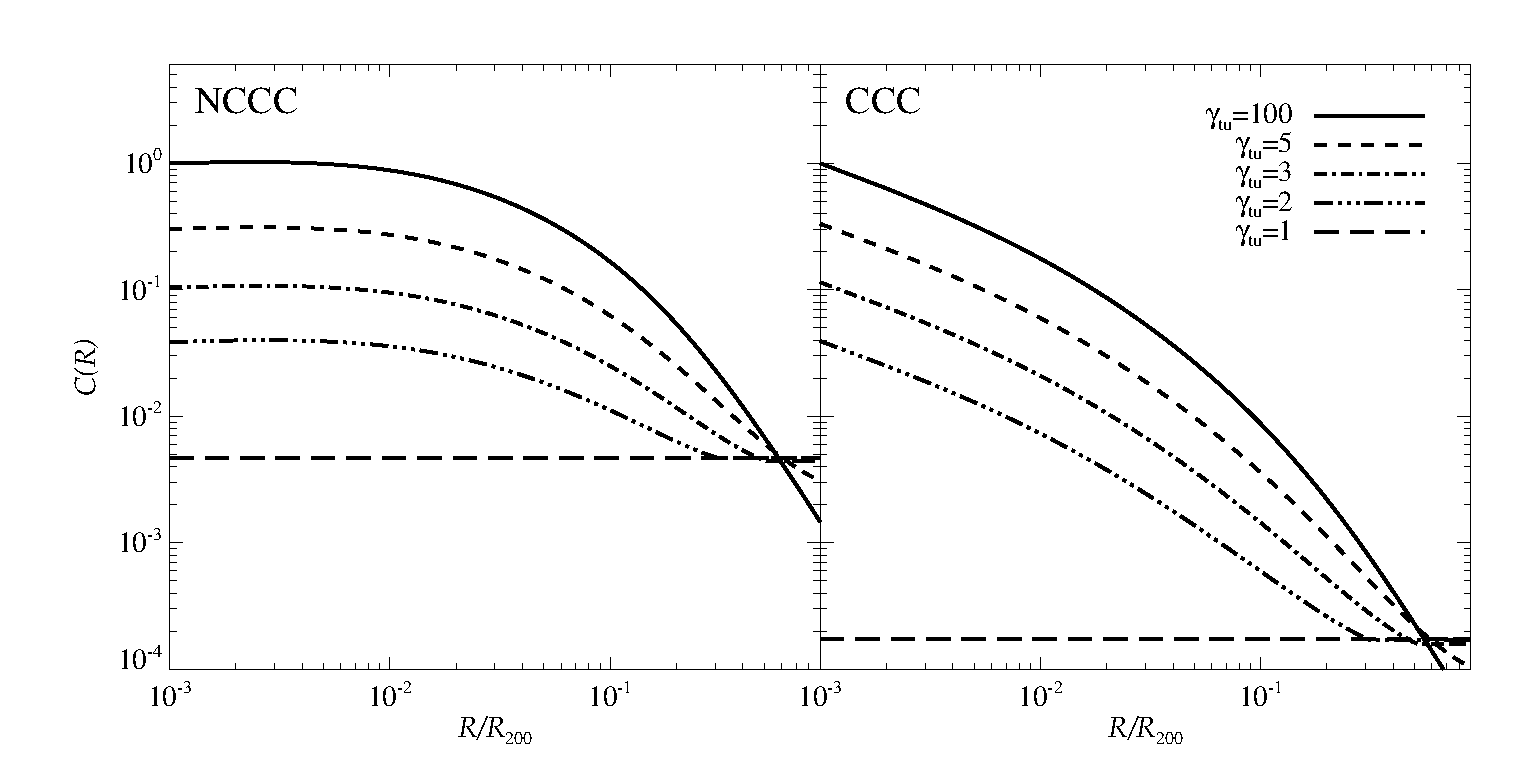
\includegraphics[width=0.62\textwidth]{figures/CR_profiles_FinalModel.eps}
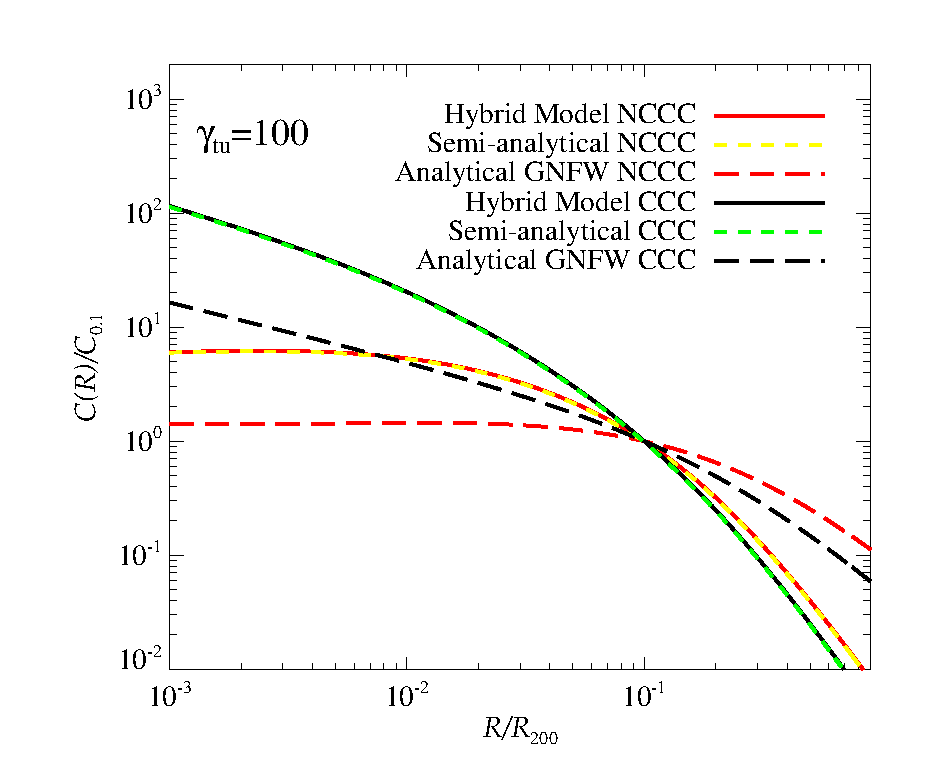
\includegraphics[width=0.37\textwidth]{figures/CR_profiles_FinalModelvsREX_norm0.1.eps}
\caption{In the left plot, our final model $C_{\rm{final}}$ is showed for the NCCC and CCC cases and for different values of $\gamma_{\rm{tu}}$. We normalize $C_{\rm{final}}$ to $C_{0}=C(0,\gamma_{\rm{tu}}=100)$ where we fix the CR populations to have a constant total CR number as in Equation~(36) of \cite{2011A&A...527A..99E} integrating up $R_{200}$. In the right plot, we compare the $C_{\rm{final}}$ and pure semi-analytical cases (plugging in our GNFW gas profiles plus the temperature outer decrease) with the analytical GNFW case (with $\alpha=2.3$) for $\gamma_{\rm{tu}}=100$. In the latter plot, the CR profiles are normalized to $C_{0.1}=C(0.1R_{200})$.}
\label{fig:CRFinalModel}
\end{figure*}

where we redefine $C_{\rm{simple}}(R)$ as $C_{\rm{final}}(R) = \tilde{C}(R) P(R) $ of our hybrid model, where $\tilde{C}(R)$ is the normalization CR profile of Equation~(22) of \cite{2010MNRAS.409..449P}, and $P(R) = n_{\rm{e}}(R) k_{\rm{B}} T(R)$. Here $T(R)$ represents the decline toward the cluster periphery expected by the fit to the universal temperature profile derived from cosmological cluster simulations \citep{2007MNRAS.378..385P,2010MNRAS.409..449P}. The last step is to generalize the case with one CR population with spectral index $\alpha$, used up to here, to the case of \cite{2010MNRAS.409..449P} where three different CR populations $\alpha_{i}=(2.15,2.3,2.55)$ are adopted. The whole formalism is easily extended to the three CR populations case by using sums over the three spectral indexes (see \citealp{2010MNRAS.409..449P}). This extension enters in the $A_{\nu}$ calculation, the $(\epsilon_{\rm{B}}(R)/\epsilon_{B_{\rm{c}}})^{(\alpha-2)/4}$ factor of Equation~(\ref{eq:surface_brightness_2}), and into Equation~(\ref{eq:Csimple_1}). While for the first two cases there are no problems, the latter would be. In fact, introducing a sum over $\alpha_{i}$ in Equation~(\ref{eq:Csimple_1}) would make impossible to analytically reverse it to get $\eta(R)$ of Equation~(\ref{eq:eta}). We decide to not introduce the three CR spectral indexes in this part and just use $\alpha = 2.3$ into Equation~(\ref{eq:Ctransport}).\footnote[9]{We check that the choice of $\alpha$ into Equation~(\ref{eq:Ctransport}) does not affect the result. Varying $\alpha$ within $2.15-2.55$ leaves the radial shape and the normalization unchanged within $0.5\%$.} We however extend to three CR spectral indexes the $A_{\nu}$ and $(\epsilon_{\rm{B}}(R)/\epsilon_{B_{\rm{c}}})^{(\alpha-2)/4}$ factors (see Appendix~\ref{app:A}). In this way, when $\gamma_{\rm{tu}}$ is high enough, e.g. 100 (1000), we recover the radial shape and normalization of the semi-analytical model of \cite{2010MNRAS.409..449P} at a $1\%$ ($0.1\%$) level.

We therefore end up with a new $C_{\rm{transport}}$, which now we shall call $C_{\rm{final}}$, with all the needed ingredients, i.e.~a mass-scaling CR normalization for our simulation derived cluster population, the general REXCESS derived GNFW gas profiles, the universal outer temperature decline and, least but not last, the $\gamma_{\rm{tu}}$ parameter which allows us to explore different turbulent states of the clusters in our MultiDark sample.\footnote[10]{In our final model, $R_{\rm{c}}$ of Equation~(\ref{eq:Rpm}) becomes the characteristic radius of our GNFW gas profile of Section~\ref{sec:2.2}, i.e.~$R_{\rm{c}}=0.2\times R_{500}$, and $\beta_{\rm{cl}}=0.8$ (changing the value of $\beta_{\rm{cl}}$ between e.g. 0.4 and 1.2 has no impact at all).}

In Figure~\ref{fig:CRFinalModel}, left plot, we show $C_{\rm{final}}$, for the NCCC and CCC cases, for different values of the $\gamma_{\rm{tu}}$ parameter. Additionally, in the right plot, we compare our final model with the analytical GNFW exact solution (see Appendix~\ref{app:B}) and the pure semi-analytical cases for $\gamma_{\rm{tu}}=100$ and normalized at $0.1 \times R_{200}$. As mentioned above, for high $\gamma_{\rm{tu}}$ values, we recover the shape and normalization of the semi-analytical model of \cite{2010MNRAS.409..449P}. Note therefore the more centrally peaked profile of our final model with respect to the analytical GNFW case. Indeed, the choice to introduce in our model $\tilde{C}$ from the \cite{2010MNRAS.409..449P} simulations may introduce a overcooling problem. This can however be easily counteracted by changing the $\gamma_{\rm{tu}}$ and $\alpha_B$ values. The risk is that, when modeling a galaxy cluster, the final $\gamma_{\rm{tu}}$ value will be biased as the CR transport effects are degenerate with the initial CR profile, the $\alpha_B$ value, and other possible effects that we are not considering here as e.g.~cluster asphericity (see also next Section).


%%%%%%%%%%%%%%%%%%%%%%%%%%%%%%%%%%%%%%%%%%%%%%%%%%%%%%%%%%%%%%%%%%%
%%%%%%%%%%%%%%%%%%%%%%%%%%%%%%%%%%%%%%%%%%%%%%%%%%%%%%%%%%%%%%%%%%%
\section{Radio Surface Brightness Modeling}
\label{sec:3}
In this Section we apply our model to reproduce the RHs characteristics of some galaxy clusters in order to show that the model adapts to different situations. In the final model we include also the \emph{maximum CR acceleration efficiency parameter} $g(\zeta_{\rm{p,max}})=g_{\rm{CR}}$ \citep{2010MNRAS.409..449P}. Note that this parameter acts just as a linear scaling for the emission and can be included in the calculation substituting $A_{\nu}$ with $A_{\nu,\rm{final}}=g_{\rm{CR}}A_{\nu}$ (see Appendix~\ref{app:A}). We warn the reader that this parameter can be compared with the value of \cite{2010MNRAS.409..449P} only when $\gamma_{\rm{tu}}\approx100$, for lower values it is just a normalization parameter and cannot be interpreted as the maximum CR acceleration efficiency. We will use instead the CR-to-thermal pressure  $X_{\rm{CR}}=P_{\rm{CR}}/P_{\rm{th}}$ as an absolute comparison parameter.\footnote[11]{We calculate the CR pressure in the following way $P_{\rm{CR}}=\frac{g_{\rm{CR}} C_{\rm{final}} m_{\rm{p}} c^{2}}{6} \Sigma_{i=1}^{3} \Delta_{i} \beta_{1/(1+q^2)}  \left( \frac{\alpha_{i}-1}{2},\frac{3-\alpha_{i}}{2} \right)$, where $c$ is the speed of light, $q=0.8$ \citep{2010MNRAS.409..449P} and $\Delta_{i} = (0.767, 0.143, 0.0975)$ are the normalization factors found by \cite{2010MNRAS.409..449P} (see also Appendix~\ref{app:A}). The thermal pressure is $P_{\rm{th}}=n_{\rm{gas}}k_{\rm{B}}T$.} 

We take as example four galaxy clusters. The giant radio halos of Coma \citep{1997A&A...321...55D} and Abell~2163 \citep{2001A&A...373..106F,2009A&A...499..679M} both merging NCCC, and the radio-mini halos of Perseus \citep{1990MNRAS.246..477P} and Ophiuchus \citep{2009A&A...499..371G,2009A&A...499..679M} both non-merging CCC. In Table~\ref{tab:RadioHalos}, we summarize the main characteristics of these halos and we detail the main parameters adopted from the modeling and results. In Figure~\ref{fig:SBmodeling}, we show the corresponding surface brightness and CR-to-thermal pressure plots. Note that we model these clusters at 1.4~GHz and within $R_{200}$. 
Let us analyze the four cases separately. 

\begin{table*}[hbt!]
\begin{center}
\caption{Radio Halos and Mini-Halos Characteristics.}
\medskip
%\begin{tabular}{c|c|c|c|c|c|c}
\begin{tabular}{cccccccc}
\hline
\phantom{\Big|}
Name & $z$ & $D$ & $\Delta d$ & $L_{1.4~\rm{GHz},~\rm{obs}}$ & Fit Parameters & $L_{1.4~\rm{GHz},~\rm{model}}$ & References \\
\phantom{\Big|}
           &   & [$h_{70}^{-1}$~Mpc] & [$h_{70}^{-1}$~Mpc] & $10^{31}$ [$h_{70}^{-2}$~erg~s$^{-1}$~Hz$^{-1}$] & $\gamma_{\rm{tu}}$, $\alpha_{\rm{B}}$ & $10^{31}$ [$h_{70}^{-2}$~erg~s$^{-1}$~Hz$^{-1}$] & \\
\hline \\[-0.5em]
Coma           & $0.023$ & $101$ & $2.15$ & $0.72$  & 1, 0.6  & 0.86 &  [1, 2, 3]   \\
               &         &       &        &                        & 4, 0.3  & 0.90  &  \\
A~2163         & $0.203$ & $962$ & $2.07$ & $15.36$     & 1, 0.3  & 13.43  &  [3, 4]  \\
\hline \\[-0.5em]
Perseus        & $0.018$ & $78$   & $0.15$ & $4.40$ & 3, 0.4   & 4.80 &  [3, 5, 6, 7]  \\
               &         &        &        &                       & 100, 0.3 & 3.97 &  \\
Ophiuchucs     & $0.028$ & $121$  & $0.41$ & $0.19$       & 5, 0.7   & 0.19  &  [3, 4] \\
               &         &        &        &                       & 100, 0.3 & 0.23 &   \\[0.5em]
\hline
\end{tabular}
\label{tab:RadioHalos}
\end{center}
\footnotesize{Note. Top rows are giant radio halos, while the bottom are mini-halos. $\Delta d$ represents the approximate dimension of the RH. $L_{1.4 GHz,~\rm{obs}}$ is the total luminosity at 1.4~GHz. $M_{200}$ and $R_{200}$ are taken, for all clusters, from \cite{2002ApJ...567..716R}. The Coma $\rho_{\rm{gas}}$ and $T$ are from \cite{1992A&A...259L..31B}, while for A~2163 and Ophiuchus they are from \cite{2002ApJ...567..716R}. For Perseus, we take $\rho_{\rm{gas}}$ from \cite{2003ApJ...590..225C} and the temperature central dip is modeled as in \cite{2004A&A...413...17P}. For all clusters, we also adopt the outer temperature decrease. Note that despite the fact that Ophiuchus is a CCC and has a central temperature dip, we adopt a constant temperature in the central part because the dip is important only below $30$~$h_{70}^{-1}$~kpc (see \citealp{2010MNRAS.405.1624M}) and therefore it is not critical for the surface brightness modeling. The Fit Parameters column indicates the best fit values (top) and other permitted values for the modeling (bottom), and $L_{1.4 GHz,~\rm{model}}$ is the corresponding predicted total luminosity at 1.4~GHz within $R_{200}$. See the main text for details. References: [1] \cite{1997A&A...321...55D} [2] \cite{1992A&A...259L..31B} [3] \cite{2002ApJ...567..716R} [4] \cite{2009A&A...499..679M} [5] \cite{1990MNRAS.246..477P} [6] \cite{2003ApJ...590..225C} [7] \cite{2004A&A...413...17P}.}
\end{table*}

\begin{figure*}[hbt!]
\centering
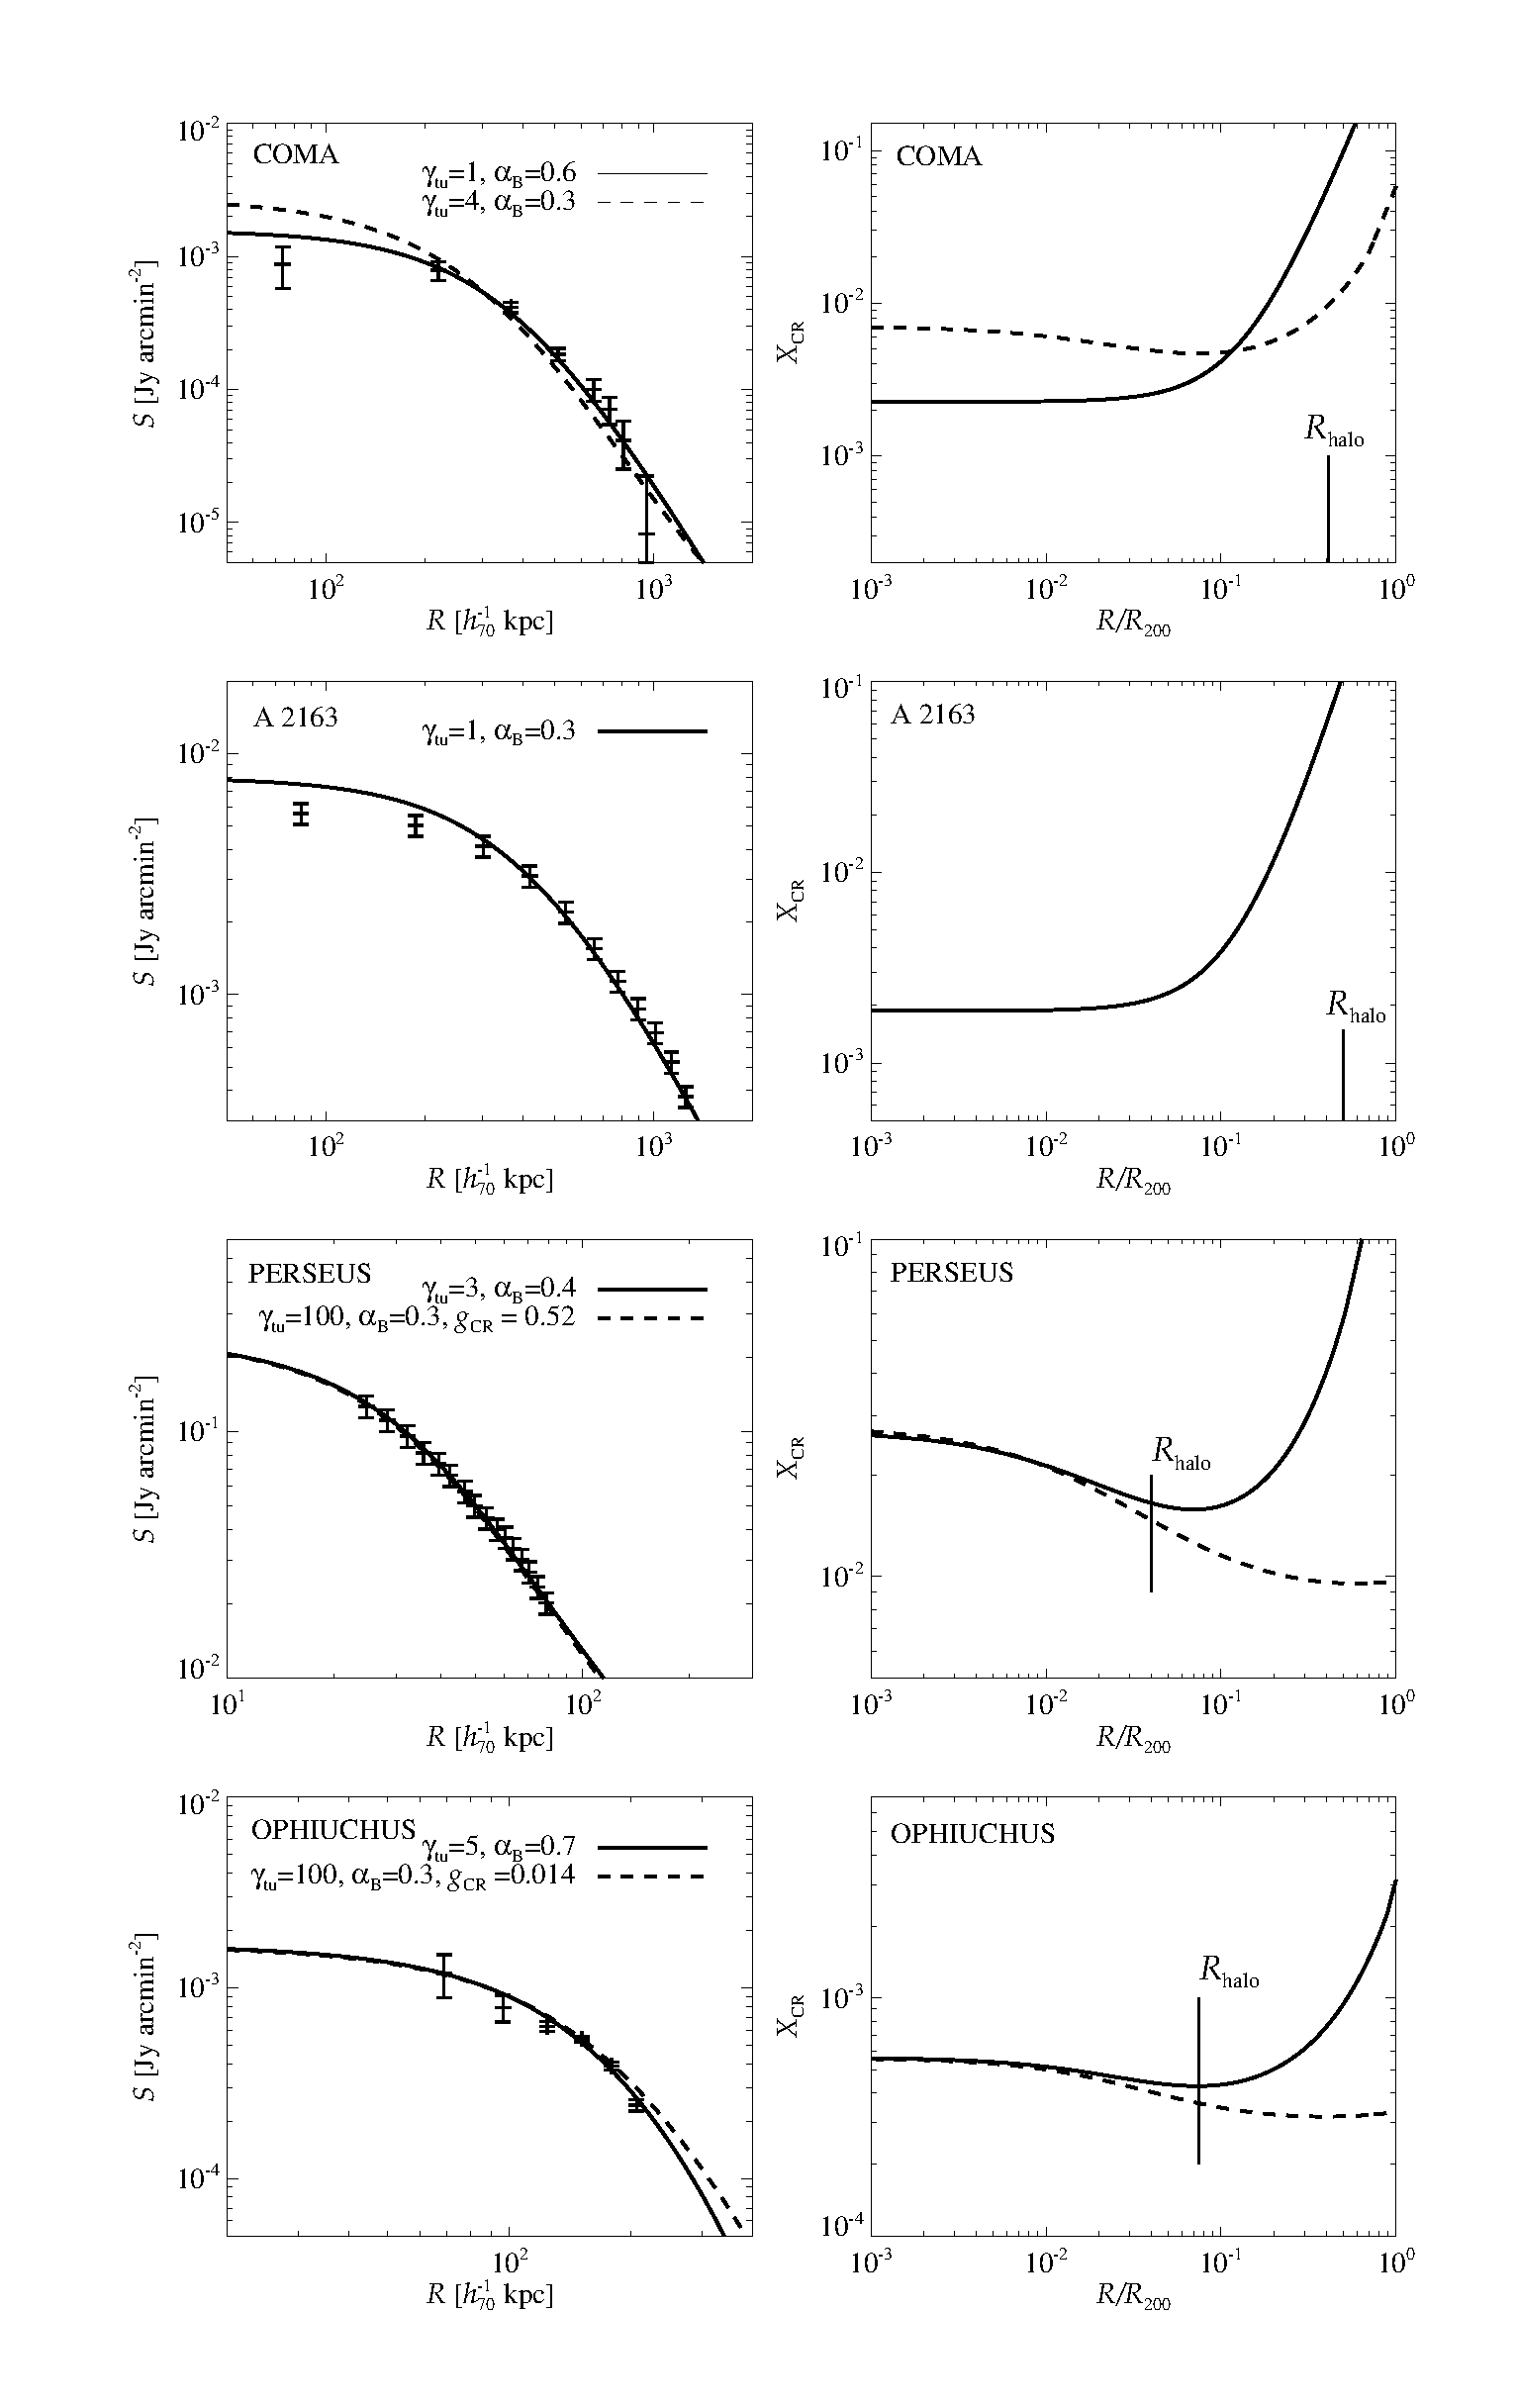
\includegraphics[width=0.78\textwidth]{figures/SB_profiles_ALL.eps}
\caption{Surface brightness modeling of the Coma, Abell~2163, Perseus and Ophiuchus RHs. Left plots show the RHs azimuthal average surface brightness, while right plots show the corresponding CR-to-thermal pressure $X_{\rm{CR}}$. Note how different parameter values, giving almost the same surface brightness shape, result in very different $X_{\rm{CR}}$ profiles. In the Abell~2163 and Ophiuchus cases we take a $10\%$ error bar instead of the errors reported by \cite{2009A&A...499..679M}. This is true also for Perseus, for which \cite{1990MNRAS.246..477P} do not report errors.}
\label{fig:SBmodeling}
\end{figure*}

The Coma giant radio halo has a morphology remarkably similar to the extended X-ray thermal bremsstrahlung emission, although the radio peak seems to be displaced by about $0.05$~deg with respect to the X-ray one and the radio emission declines more slowly going toward the cluster outskirts \citep{1992A&A...259L..31B,1997A&A...321...55D}. Note that it is clearly non-spherical, showing an elongation in the East-West direction. The \cite{1992A&A...259L..31B} X-ray observations were performed with the ROSAT satellite which had a resolution between $0.0028$ and $0.008$~deg depending on the pointing mode. The full width half maximum (FWHM) of the \cite{1997A&A...321...55D} radio observation beam was $0.156$~deg, so almost two orders of magnitude larger than the X-ray observation\footnote[12]{Note therefore that the difference in position of the radio and X-ray peaks is negligible for the modeling.}. This can of course have a critical impact on the modeling. We decide therefore to apply a Gaussian smoothing to our theoretical surface brightness of Equation~(\ref{eq:surface_brightness_1}) with $\sigma_{\rm{smoothing}} = FWHM_{\rm{radio}}/2.355$. We investigate different values of $\alpha_{\rm{B}}=(0.3,0.4,0.5,0.6,0.7)$ and of the $\gamma_{\rm{tu}}$ parameter from 1 to 100.\footnote[13]{We fix the CR number for $\gamma_{\rm{tu}}=100$ using Equation~(36) of \cite{2011A&A...527A..99E}, integrating up $R_{200}$, and then we oblige the CR number to be the same at lower $\gamma_{\rm{tu}}$ values.} We fix the central magnetic field $B_{0}=5$~$\mu$G \citep{2010A&A...513A..30B} and we use $g_{\rm{CR}}$ as normalization factor to match the radio observations. The best fit to the data is obtained for $\gamma_{\rm{tu}}=1$ and $\alpha_{\rm{B}}=0.6$, however, values as high as $\gamma_{\rm{tu}} \approx 4$ could be accommodated. We can recover the radio surface brightness shape and the total radio luminosity within about $20\%$. The gamma-ray flux (calculated as described in Appendix~\ref{app:C}), within $R_{200}$, for the best fit case and for energies above 100~MeV (100~GeV) is $F_{\gamma} = 4.1 \times 10^{-9}$~cm$^{-2}$~s$^{-1}$ ($1.5 \times 10^{-12}$~cm$^{-2}$~s$^{-1}$). The $\gamma_{\rm{tu}} = 1$ case is therefore in tension with the limit recently set by \emph{Fermi}-LAT \citep{2012AAS...21920701Z} of $F_{\gamma, UL} (>100~\rm{MeV}) \approx 2.5 \times 10^{-9}$~cm$^{-2}$~s$^{-1}$. We note that using a slightly higher $\gamma_{\rm{tu}}$ value the predictions become again in agreement with gamma-ray observations. In fact, for $\gamma_{\rm{tu}} = 4$ and $\alpha_{\rm{B}}=0.3$ one obtains $F_{\gamma} (>100~\rm{MeV}) = 9.6 \times 10^{-10}$~cm$^{-2}$~s$^{-1}$ ($F_{\gamma} (>100~\rm{GeV}) = 3.6 \times 10^{-13}$~cm$^{-2}$~s$^{-1}$). 

The Abell~2164 giant radio halo is also closely correlated to the cluster thermal X-ray structure showing, as in the Coma case, a slower decline going toward the cluster outskirts with respect to the bremsstrahlung emission \citep{2001A&A...373..106F}. It also appears to be non-spherical, being its shape clearly elongated in the East-West direction. The radio observations of \cite{2001A&A...373..106F} were performed with the Very Large Array (VLA with) a corresponding synthesized beam of $45$''$\times60$'' at 1.4 ~GHz. For our modeling we use the surface brightness provided in \cite{2009A&A...499..679M} where the radio image has been convolved with a circular Gaussian beam and corrected for the primary beam attenuation, resulting in a $FWHM_{\rm{radio}}=62$"=$0.017$~deg. We note that the position of radio and X-ray peaks are displaced by about 19''. Matteo Murgia has kindly provided the radio surface brightness computed with respect to the \cite{2002ApJ...567..716R} X-ray position, however it is almost unchanged with respect to the original. The $FWHM_{\rm{radio}}$ is larger than the resolution of the ROSAT satellite from which we take the gas density, even if not critically like in the Coma case. However, once converted the angular sizes to physical sizes, the corresponding $\sigma_{\rm{smoothing}}$ is of the order of the Coma one because of the high distance of Abell~2163. Therefore, we apply a Gaussian smoothing also in this case. We follow the same procedure as in Coma, using again $B_{0}=5$~$\mu$G. The best fit to the data, and also the only acceptable one, is obtained for $\gamma_{\rm{tu}}=1$ and $\alpha_B=0.3$, i.e.~the flattest possible surface brightness. We can recover the emission shape and the total luminosity within about $15\%$. The corresponding gamma-ray flux, within $R_{200}$, for energies above 100~MeV (100~GeV) is $F_{\gamma} = 4.2 \times 10^{-10}$~cm$^{-2}$~s$^{-1}$ ($1.5 \times 10^{-13}$~cm$^{-2}$~s$^{-1}$), about two orders of magnitude lower than the upper limit obtained by \emph{Fermi}-LAT \citep{2010ApJ...717L..71A}.

The Perseus diffuse radio emission is probably the most famous example of radio-mini halo \citep{1990MNRAS.246..477P} and Perseus itself is surely the best studied cluster in X-rays (e.g.~\citealp{2003ApJ...590..225C,2006MNRAS.366..417F,2011arXiv1105.5025F}). Also in the Perseus case, clear similarities between radio and thermal X-ray structures are found. One of the strengths of the hadronic model for RHs is that it naturally predicts mini-halos as a consequence of the more peaked gas density in CCC with respect to the radio halos found in NCCC, as we will see now. 
We proceed as before but now adopting $B_{0}=10$~$\mu$G (see \citealp{2010ApJ...710..634A,2011arXiv1111.5544M} for a discussion on the Perseus magnetic field). 
The best fit to the data is obtained for $\gamma_{\rm{tu}}=3$ and $\alpha_{\rm{B}}=0.4$, however, values as high as $\gamma_{\rm{tu}} \approx 100$, and as low as $\gamma_{\rm{tu}}=2$, could be easily accommodated. We can recover the surface brightness shape and the total luminosity within about $10\%$. The gamma-ray flux, within $R_{200}$, for the best fit case and for energies above 100~MeV (100~GeV) is $F_{\gamma} = 1.4 \times 10^{-8}$~cm$^{-2}$~s$^{-1}$ ($5.1 \times 10^{-12}$~cm$^{-2}$~s$^{-1}$). Adopting $\gamma_{\rm{tu}}=100$ and $\alpha_B=0.3$, the corresponding gamma-ray flux above 100~MeV (100~GeV) is $F_{\gamma} = 4.9 \times 10^{-9}$~cm$^{-2}$~s$^{-1}$ ($1.8 \times 10^{-12}$~cm$^{-2}$~s$^{-1}$). We note that the central galaxy NGC~1275 flux above 100~MeV measured by \emph{Fermi} is of about $2 \times 10^{-7}$~cm$^{-2}$~s$^{-1}$ \citep{2009arXiv0904.1904T}, well above our predictions that however refer to the whole cluster. We can compare these predictions with the upper limit above 1~TeV, and for a region within $0.15$~deg around the cluster center, recently obtained by \cite{2011arXiv1111.5544M}. We predict for the $\gamma_{\rm{tu}}=3$ ($\gamma_{\rm{tu}}=100$) case a flux of $F_{\gamma}(>1~\rm{TeV},<0.15~\rm{deg}) = 7.3 \times 10^{-14}$~cm$^{-2}$~s$^{-1}$ ($5.5 \times 10^{-14}$~cm$^{-2}$~s$^{-1}$), which is well below the MAGIC collaboration upper limit of $F_{\gamma,\rm{UL}}(>1~\rm{TeV},<0.15~\rm{deg}) \approx 1.4 \times 10^{-13}$~cm$^{-2}$~s$^{-1}$. Note also that, in the case of $\gamma_{\rm{tu}} = 100$, we need a maximum CR acceleration efficiency parameter of $0.52$, about half of the value adopted by \cite{2010MNRAS.409..449P} (note that we do not obtain the same luminosities predicted by \cite{2010MNRAS.409..449P} because they do not use the temperature central dip and outer decrease).

The Ophiuchus cluster has been widely studied both in radio and X-rays in the last few years because of a claim of presence of a non-thermal hard X-ray tail \citep{2008A&A...479...27E,2008PASJ...60.1133F,2009A&A...499..371G,2009A&A...499..679M,2009MNRAS.396.2237P,2009A&A...508.1161N,2010A&A...514A..76M,2010MNRAS.405.1624M}. It was classified as a merging cluster by \cite{2001PASJ...53..605W}, but more recently \cite{2008PASJ...60.1133F} did not found any evidence of merging and, on the contrary, classified it as one of the hottest clusters with a  cool-core (see also \citealp{2010MNRAS.405.1624M}). The subsequent discovery of the radio mini-halo by \cite{2009A&A...499..371G} confirmed the cool-core nature of this cluster, also founding similarities with the thermal X-ray emission. For our modeling we use the surface brightness provided by \cite{2009A&A...499..679M}.  The presence in Ophiuchus of a strong central cD galaxy is also typical of CCC.
We note that also in this case, the position of radio and X-ray peaks seems displaced by about 24''. Again, Matteo Murgia has kindly provided the radio surface brightness computed with respect to the \cite{2002ApJ...567..716R} X-ray position, however the change is not very significant with respect to the original. 
We proceed as before, adopting a central magnetic field value of $B_{0}=10$~$\mu$G.
The best fit to the data is obtained for $\gamma_{\rm{tu}}=5$ and $\alpha_B=0.7$, however, values as high as $\gamma_{\rm{tu}} \approx 100$, and as low as $\gamma_{\rm{tu}}=2$, could be easily accommodated. We can recover the surface brightness shape and the total luminosity within about $20\%$. The gamma-ray flux, within $R_{200}$, for the best fit case and for energies above 100~MeV (100~GeV) is $F_{\gamma} = 1.2 \times 10^{-10}$~cm$^{-2}$~s$^{-1}$ ($4.3 \times 10^{-14}$~cm$^{-2}$~s$^{-1}$). Adopting $\gamma_{\rm{tu}}=100$ and $\alpha_B=0.3$, the corresponding gamma-ray flux above 100~MeV (100~GeV) is $F_{\gamma} = 8.3 \times 10^{-11}$~cm$^{-2}$~s$^{-1}$ ($3.1 \times 10^{-14}$~cm$^{-2}$~s$^{-1}$). The gamma-ray flux is, in both cases, about two orders of magnitude lower than the upper limit obtained by \emph{Fermi}-LAT \citep{2010ApJ...717L..71A}. Note also that, in the case of $\gamma_{\rm{tu}} = 100$, we obtain a maximum CR acceleration efficiency parameter of $0.014$. 

We want to stress the following points:
\begin{enumerate} 
 \item The giant radio halos of Coma and Abell~1263 are more difficult to reproduce than the mini-halos. 
       We need in fact very low $\gamma_{\rm{tu}}$ values in order to get acceptable fits.
       We would expect higher $\gamma_{\rm{tu}}$ values for the merging NCCC cases \citep{2011A&A...527A..99E}.
       However, there are three main factors that render the merging NCCC fits not conclusive and can alleviate this problem. 
       i) Primary electrons accelerated in outer shocks, which we do not consider, could have an important contribution in the RH emission.
       ii) Merging clusters are not spherical symmetric, and this is clearly the case both for Coma and Abell~2163.
       Finally, iii) adopting the simulation-driven $\tilde{C}$ from \cite{2010MNRAS.409..449P} in constructing our hybrid model, 
       we may be adopting a too steep central CR normalization which would result in lower required $\gamma_{\rm{tu}}$ values with respect to a 
       smoother choice. To test this last point, we fitted the Coma surface brightness using a model without $\tilde{C}$ from \cite{2010MNRAS.409..449P} obtaining  
       that values as high as $\gamma_{\rm{tu}} \approx 8$ could be accommodated. However, the $\gamma_{\rm{tu}}=1$ case still represents the best fit model, it is
       indeed not affected by such arguments as the CR profile is always flat in this case. Despite these issues, we can reproduce the Coma and Abell~2163 RHs 
       fairly well, solving the previous problems of the \emph{classical} hadronic model (see e.g.~\citealp{2010MNRAS.401...47D}). 
 \item Generally, RHs measurements set more stringent constraints on the hadronic model than gamma-ray observations, see e.g.~Perseus. 
       This is not always true, in fact, the gamma-ray limit by \emph{Fermi}-LAT set the strongest constraint in the Coma cluster case.
       We do not intend to discourage gamma-ray observations by any means. On the contrary, they are a fundamental tool in this field being 
       independent from the choices we make here to reproduce their nature. However, previous gamma-ray predictions should be scaled down
       in light of the results presented here (see also \citealp{2011A&A...527A..99E}).
 \item The magnetic field values adopted here are perfectly in agreement with other observational constrains, solving previous tensions of the \emph{classical}
       hadronic model (see e.g.~\citealp{2011ApJ...728...53J}). We note also that very different $B_{0}$ values could be adopted without entering 
       in tension with other observational constraints. The only exception is Coma for which a higher $B_{0}$ value may be in contradiction 
       with \cite{2010A&A...513A..30B}, while a lower one could result in a higher gamma-ray emission in contrast with the \cite{2012AAS...21920701Z}
       limit.
 \item When reducing to the $\gamma_{\rm{tu}}=100$ case, which is plausible only for Perseus and Ophiuchus, the $g_{\rm{CR}}$ parameter can be interpreted as the maximum
       CR acceleration efficiency used in \cite{2010MNRAS.409..449P}. This value should then be universal, i.e.~it should be the same in all clusters. We find 
       $g_{\rm{CR, Perseus}} = 0.52$ and $g_{\rm{CR, Ophiuchus}} = 0.014$, because we fixed $B_{0}=10$~$\mu$G in both cases and used $g_{\rm{CR}}$ as normalization. This 
       discrepancy can be solved by highering/lowering the Perseus/Ophiuchus central magnetic field (e.g.~$B_{0,\rm{Perseus}}=20$~$\mu$G and 
       $B_{0,\rm{Ophiuchus}}=1$~$\mu$G). We note however that, at this stage, this is not conclusive by any means as any $\gamma_{\rm{tu}}$ value can 
       virtually be chosen for both clusters. 
 \item With this cluster sample, we cannot draw any definitive conclusion on the parameters used in the modeling as many different choices could be done on
       the magnetic field, the $\gamma_{\rm{tu}}$ and $\alpha_{\rm{B}}$ parameters. This is particularly true for the analyzed mini-halos, for which almost all the
       ($\gamma_{\rm{tu}}$, $\alpha_{\rm{B}}$) parameter space is available (note also the the $\gamma_{\rm{tu}}$ and $\alpha_{\rm{B}}$ variable are of course degenerate). This 
       would probably not change using all the knows RHs, however such a comprehensive work is highly desirable. This is beyond the scope of this work with which instead we 
       want to investigate the LOFAR cluster survey potentiality in this sense.
\end{enumerate}

We conclude saying that the model presented here is versatile enough to adapt do very different situations, reproducing the main characteristics of RHs and. As we will see in
the next section, it can also reproduce the radio-to-X-ray, solving the previous problems of the \emph{classical} hadronic model, and radio-to-SZ scaling relations. It therefore fully accomplishes to our initial purposes.

\begin{figure*}[hbt!]
\centering
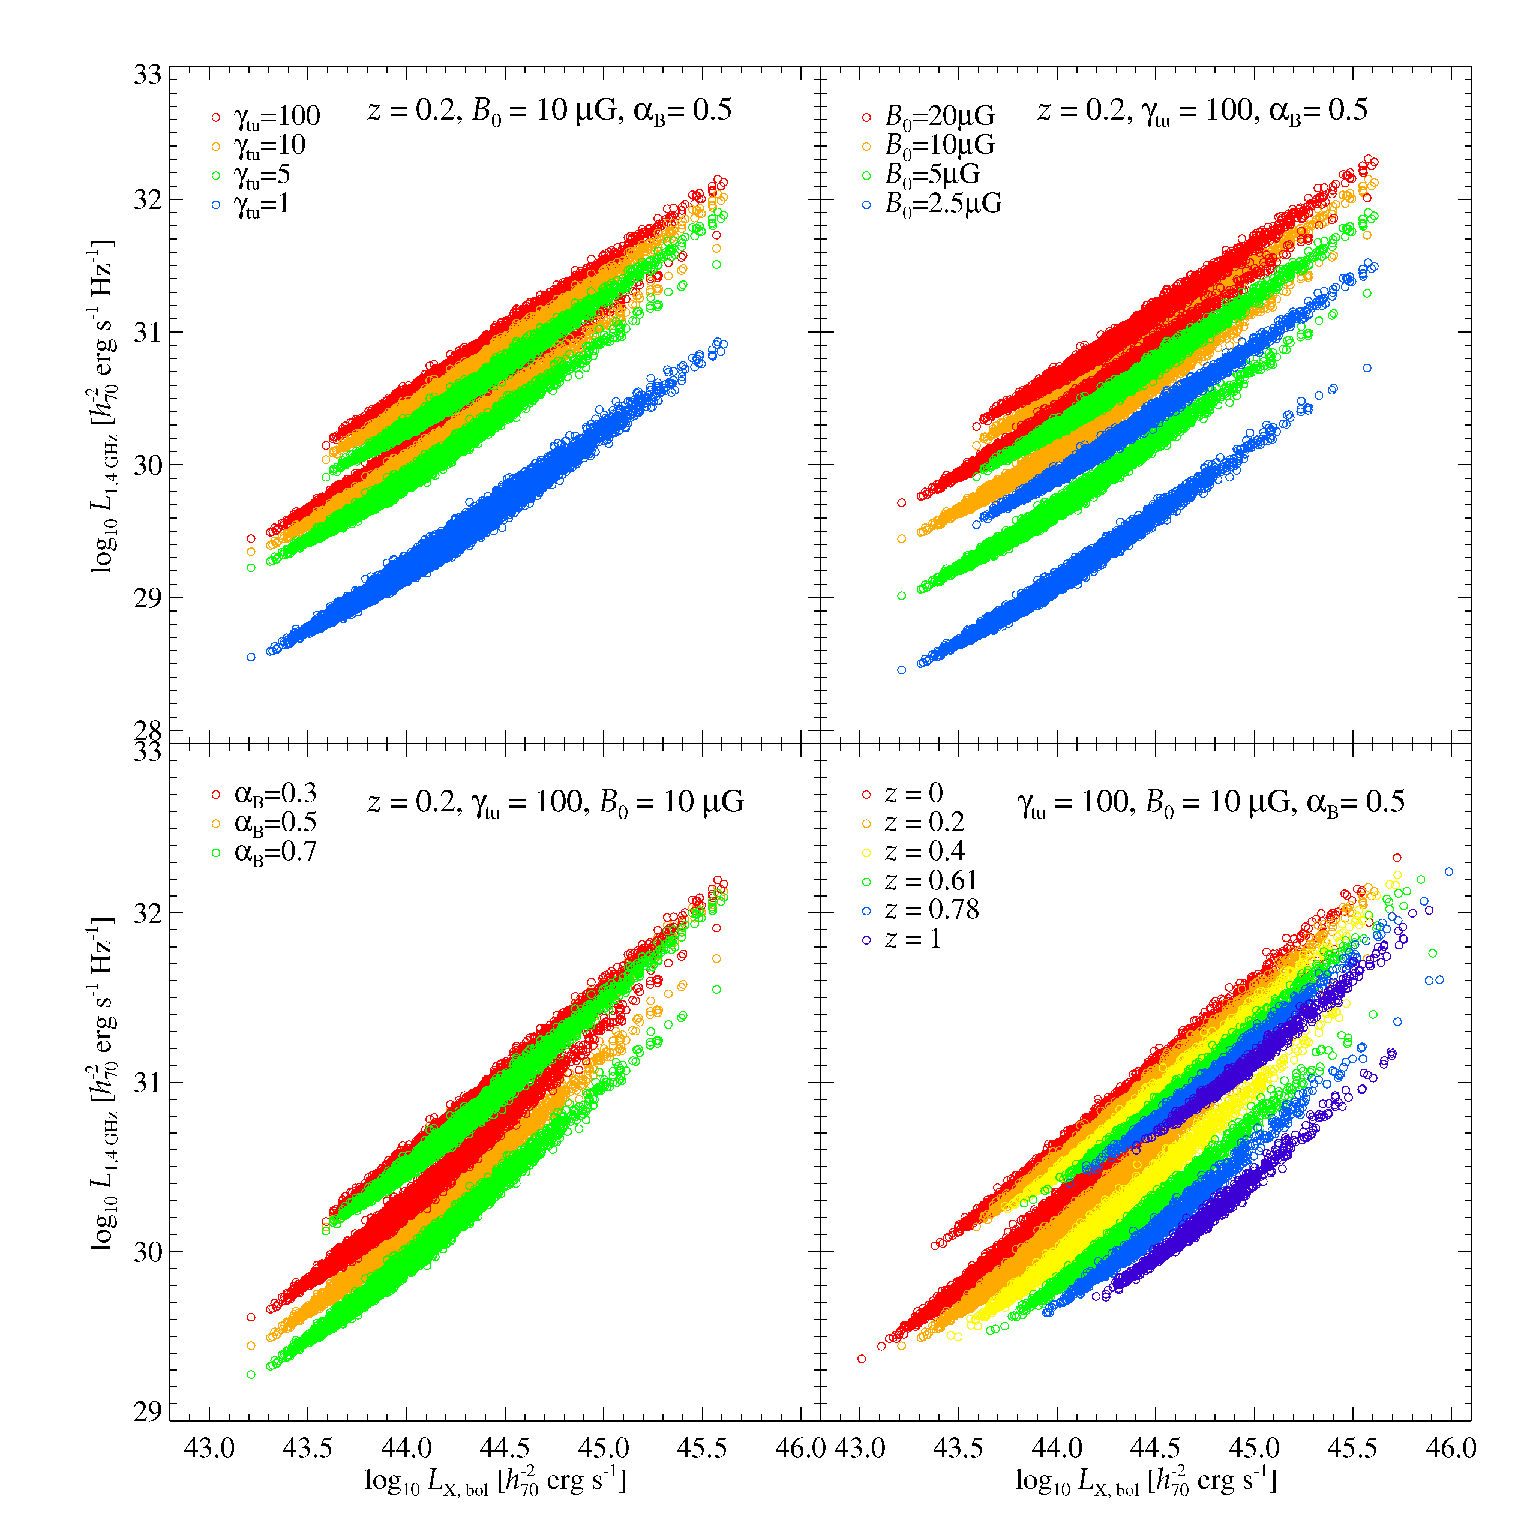
\includegraphics[width=0.49\textwidth]{figures/PL_relation_testing_gimp.eps}
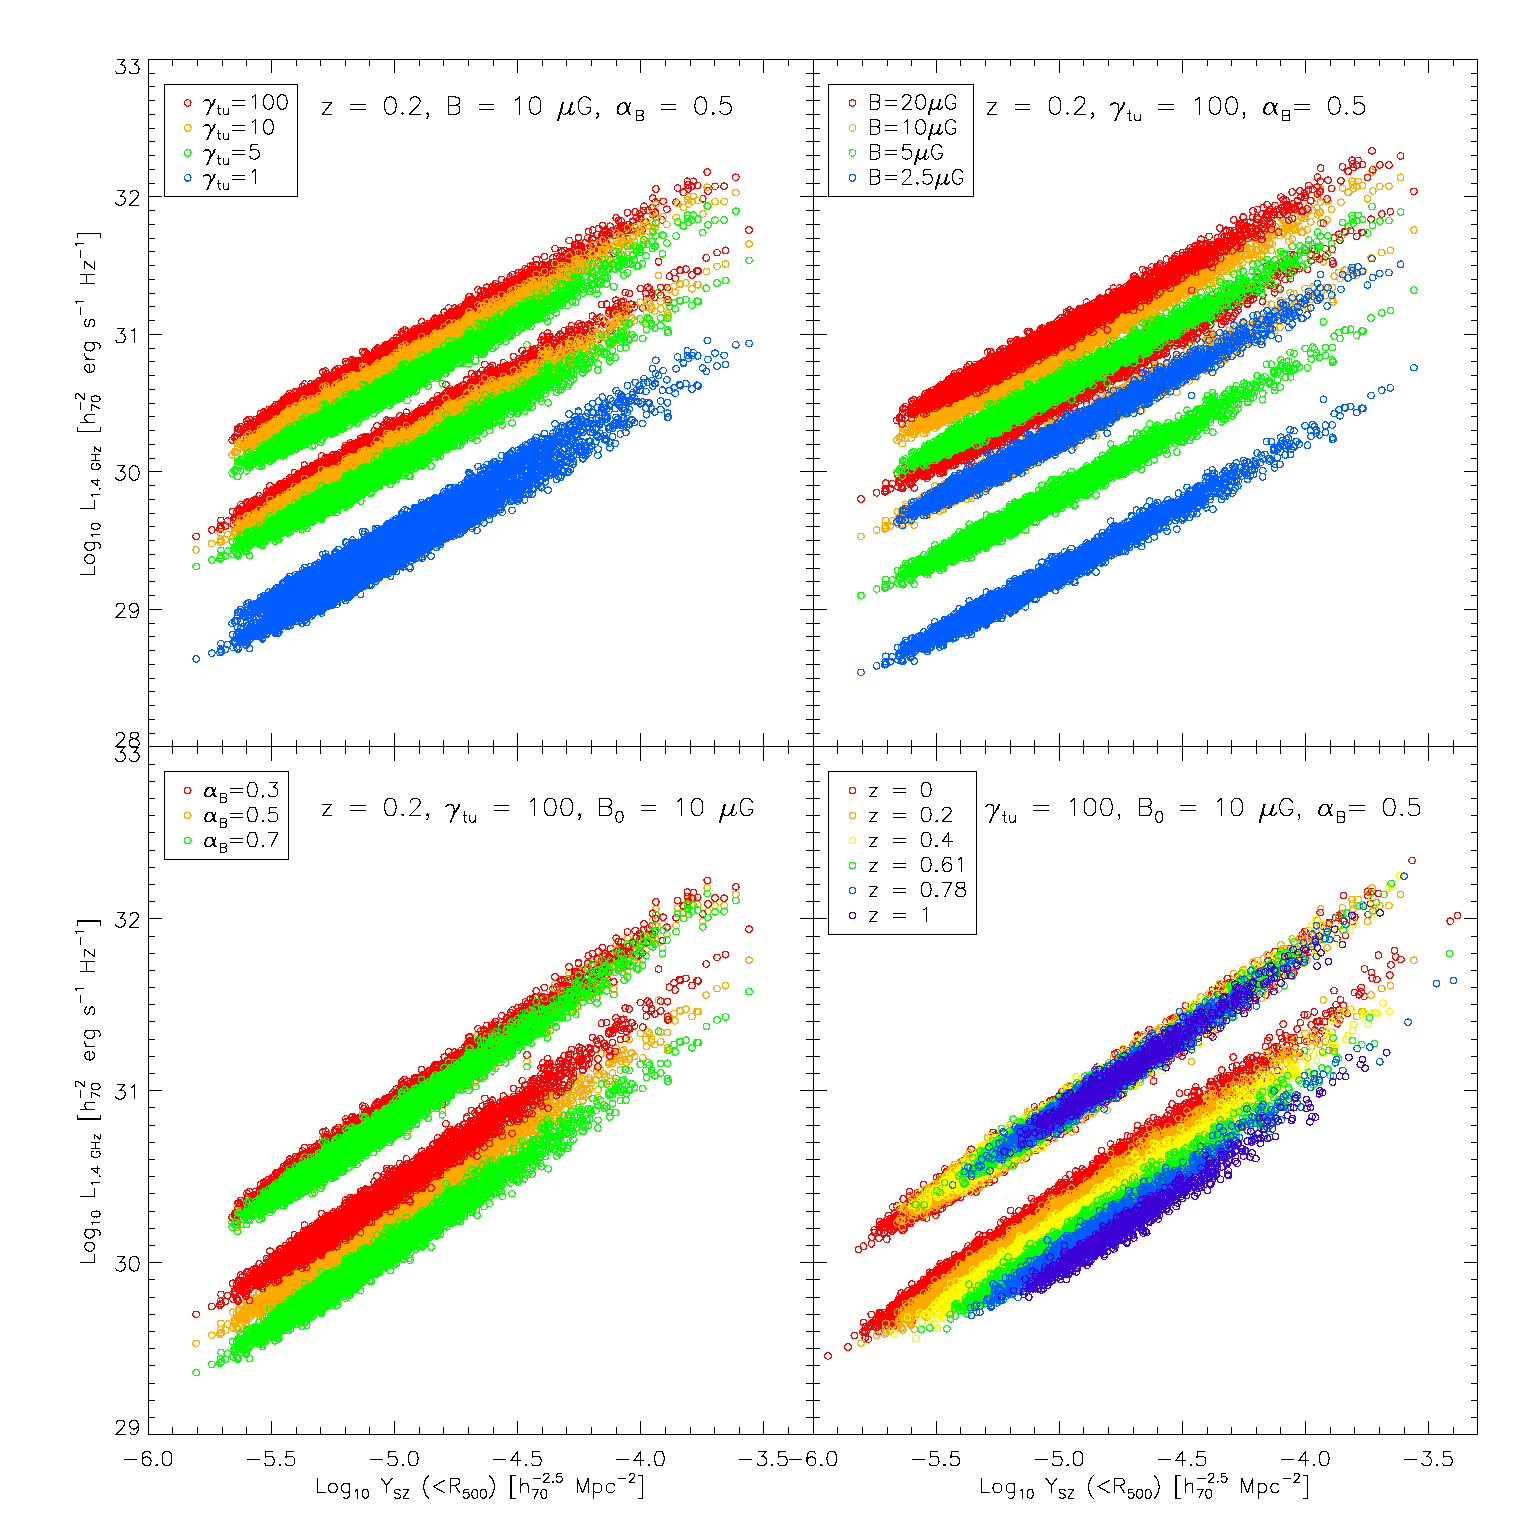
\includegraphics[width=0.49\textwidth]{figures/PSZ_relation_testing_gimp.eps}
\caption{Radio-to-Xray and radio-to-SZ general scaling relations as predicted by our final CR model. In the left panel, we show how the $L_{1.4~\rmn{GHz}}-L_{\rm{X,bol}}$ relation changes changing different parameters. In the right panel, we show the same but for the $L_{1.4~\rmn{GHz}}-Y_{\rm{SZ},500}$ relation. Note that in each plot there are two separated populations for each model realization, the top one is the CCC population while the bottom one is the NCCC population. The text in the plots indicates the parameters which are kept fixed. We fix the $g_{\rm{CR}}$-normalization parameter to 0.5 for all cases. See main text for details. {\bf change colors?}}
\label{fig:SR}
\end{figure*}

%%%%%%%%%%%%%%%%%%%%%%%%%%%%%%%%%%%%%%%%%%%%%%%%%%%%%%%%%%%%%%%%%%%
%%%%%%%%%%%%%%%%%%%%%%%%%%%%%%%%%%%%%%%%%%%%%%%%%%%%%%%%%%%%%%%%%%%
\section{Radio Scaling Relations and Luminosity Function}
\label{sec:4}
An anticipated in the Introduction, there exist an apparent bimodality between the radio and X-ray cluster emission. Clusters with the same X-ray luminosity both host RHs and do not show any diffuse radio emission (e.g.~\citealp{2009A&A...507..661B,2011A&A...527A..99E}). However, more recently, a study of the radio-to-SZ scaling relation showed the absence of any kind of strong bimodality dividing the cluster population into radio-loud and radio-quiet clusters \citep{2012MNRAS.421L.112B}. In this section, we investigate these two scaling relations and subsequently the radio luminosity function (RLF).

In Figure~\ref{fig:SR}, we show the general scaling relations of our final CR model of Section~\ref{sec:2.3} applied to the MultiDark sample. We show both the radio-to-X-ray  and the radio-to-SZ scaling relations varying different parameters as $\gamma_{\rm{tu}}$, $B_{0}$, $\alpha_{\rm{B}}$ and the redshift. We fix the $g_{\rm{CR}}$-normalization parameter to 0.5 for all cases, ensuring an average CR-to-thermal pressure at $2\%$-level ($0.05\%$-level) within $R_{500}$ ($R_{500}/2$). Here, the radio luminosity is calculated within $R_{500}$ and at $1.4$~GHz and it will be in the following unless differently specified.\footnote[14]{The median (mean) difference between calculating $L_{1.4~\rm{GHz}}$ within $R_{200}$ or $R_{500}$ is 5.6\% (5.3\%).} In our CR model, we fix the CR number for $\gamma_{\rm{tu}}=100$ using Equation~(36) of \cite{2011A&A...527A..99E}, integrating up $R_{500}$, and then we oblige the CR number to be the same at lower $\gamma_{\rm{tu}}$ values; this will be the case also in the following unless differently specified. Note in particular how the different parameters affect in different ways the NCCC and CCC populations for the $L_{1.4~\rmn{GHz}}-L_{\rm{X,bol}}$ and $L_{1.4~\rmn{GHz}}-Y_{\rm{SZ}}$ relations. This is mainly the result of the different dependence on gas density of $L_{\rm{X}}$ and $Y_{\rm{SZ}}$.

We want now to compare our model prediction directly with observations. For this purpose, we select a particular realization of our model as representative. We artificially, and randomly, divide our MultiDark $z=0.2$ sample (which well compares with the redshift of the observational samples, see below and Appendix~\ref{app:D}) in radio-quiet and radio-loud clusters, with the latter being $10\%$ of the total (as approximately found by \citealp{1999NewA....4..141G}). We assign $\gamma_{\rm{tu}}=1$ to all the radio-quiet cluster, and we assign randomly and uniformly distributed central magnetic fields $B_0$ in the intervals $[2.5,5.5]$~$\mu$G and $[5,10]$~$\mu$G for NCCC and CCC clusters, respectively. For the radio-loud clusters, we assign randomly and uniformly $\gamma_{\rm{tu}}$ values in the intervals $[40,80]$ and $[1,5]$ for NCCC and CCC clusters, respectively, and central magnetic field values in the intervals $[4.5,7.5]$~$\mu$G and $[7.5,12.5]$~$\mu$G for NCCC and CCC clusters, respectively. We fix $\alpha_{\rm{B}}=0.5$. Also here, we adopt a $g_{\rm{CR}}$-normalization parameter value of 0.5, ensuring the median average CR-to-thermal pressure of about $2\%$ ($0.05\%$) within $R_{500}$ ($R_{500}/2$). We warn the reader that these choices are not driven by any consideration apart the need to reproduce observations. Indeed, we have no robust clues at all of which values should take these parameters in clusters, with possibly the only exception of the magnetic field. Indeed, it is clear the need of large population studies of radio observed clusters in order to be able to draw robust hypothesis on the interplay of the different parameters in the modeling. In Figure~\ref{fig:PLSZ}, we show how our model prediction compares with the observed radio-to-X-ray and radio-to-SZ scaling relations. Let us first comment on the two observational relations.

\begin{figure*}[hbt!]
\centering
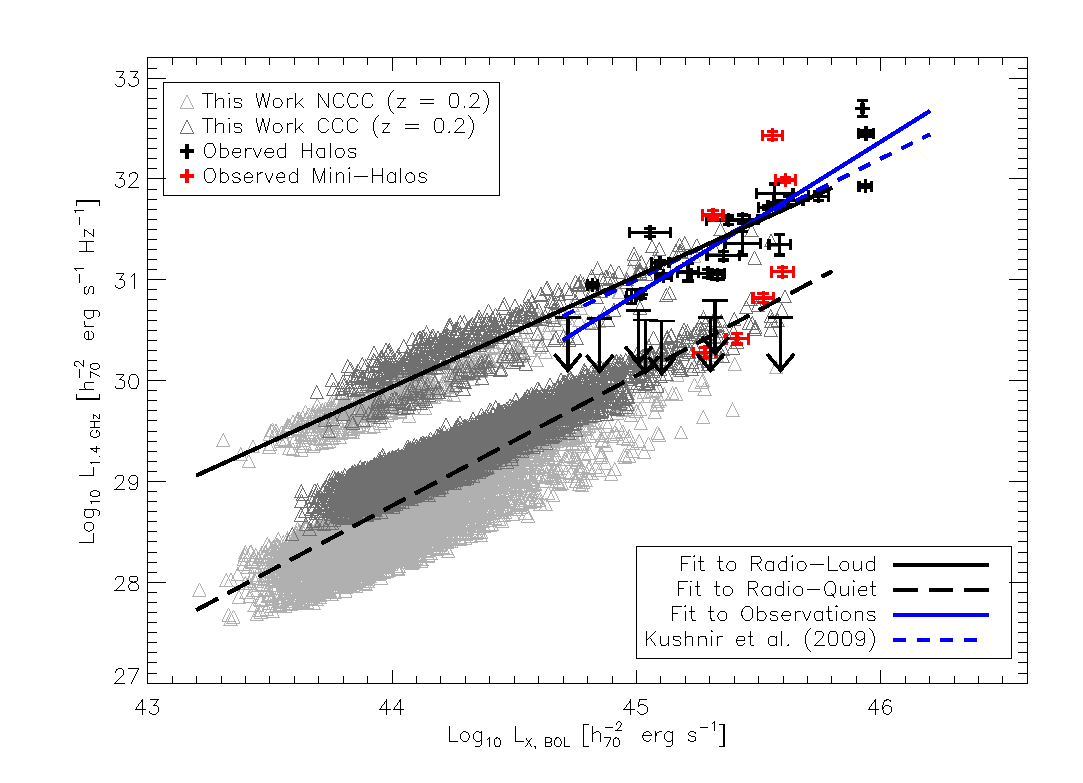
\includegraphics[width=0.49\textwidth]{figures/PL_relation.eps}
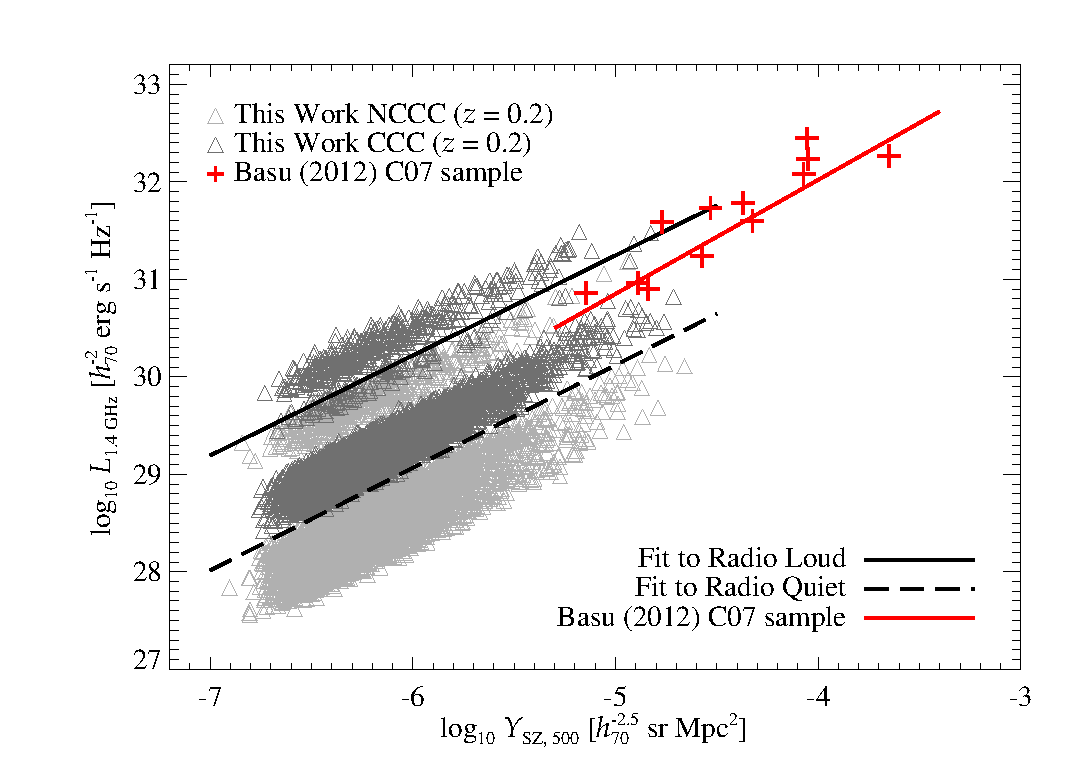
\includegraphics[width=0.49\textwidth]{figures/PSZ_relation.eps}
\caption{Radio-to-X-ray and radio-to-SZ scaling relation predictions from our final CR model (see main text for the details of the chosen parameters) compared with observations.
Left: $L_{1.4~\rmn{GHz}}-L_{\rm{X,bol}}$ prediction compared to the observational sample constructed in Appendix~\ref{app:D}. Right: $L_{1.4~\rmn{GHz}}-Y_{\rm{SZ}}$ prediction compared to the observational sample C07 from \cite{2012MNRAS.421L.112B}.}
\label{fig:PLSZ}
\end{figure*}
 
For comparison with the observed 1.4~GHz radio-to-X-ray scaling relation, in Appendix~\ref{app:D}, we construct the sample shown as black (halos) and red (mini-halos) crosses (plus some upper limits) in the left plot of Figure~\ref{fig:PLSZ}. This sample is obtained mainly from \cite{2009A&A...507..661B}, \cite{2011A&A...527A..99E},  and \cite{2009A&A...499..371G} and has a median redshift of $z\approx0.18$. The corresponding observational scaling relation in the form of $\log_{10} L_{1.4~\rmn{GHz}}~[h_{70}^{-2}~\rmn{erg}~\rmn{s}^{-1}~\rmn{Hz}^{-1}] = A + B~\log_{10} L_{\rm{X,bol}}~[h_{70}^{-2}~\rmn{erg}~\rmn{s}^{-1}]$ has $A=-50.433\pm2.226$ and $B=1.803\pm0.049$, and a scatter of $\sigma_{yx} \approx 0.44$ (note that we do not include upper limits in the fit). We refer the reader to \cite{2009A&A...507..661B} and \cite{2011A&A...527A..99E} for an extensive discussion on this topic. However, before to proceed, we would like to stress that, as interestingly noted also by \cite{2009A&A...499..679M}, in contrast with radio halos, mini-halos seem to span a wide range of radio luminosity. The Perseus mini-halo (Y-axis highest red cross in the left plot of Figure~\ref{fig:PLSZ}), for example, has a radio luminosity which is almost two order of magnitude higher than radio halos at the same X-ray luminosity. On the other hand, the Ophiuchus mini-halo (Y-axis lowest red cross in the left plot of Figure~\ref{fig:PLSZ}), which is a representative of other few such examples recently detected in CCC (i.e.~A2029 and A1835), has a radio luminosity which is much lower, more typical of halos in merging clusters, and actually below the shown upper limits. We also want to stress that, in our opinion, the slope of the $L_{1.4}-L_{\rm{X,bol}}$ relation is far from being clearly determined because of the few known RHs and the uncertainties in the measurements both in the radio  and X-ray domains. The recently detected mini-halos with very low luminosities are a clear example of the uncertainty and the wide scatter that this relation can have. On the other hand, e.g.~X-ray luminosities from ROSAT and \emph{Chandra} for the same objects can easily differ by a factor of 2 or more sometimes. In Figure~\ref{fig:PLSZ} left plot, we additionally show the \cite{2009JCAP...09..024K} slope prediction of $\approx1.2$, arbitrarily normalized for visual purposes, from their simple analytical hadronic model.

For the comparison to the observed 1.4~GHz radio-to-SZ scaling relation, we take as reference the result obtained by \cite{2012MNRAS.421L.112B} with the sample of radio halos from \cite{2007MNRAS.378.1565C} (hereafter C07; median redshift of $z \approx 0.18$; note that no mini-halos are included). For this sample, \cite{2012MNRAS.421L.112B} quotes $Y_{\rm{SZ}}$ within the halo radii given by \cite{2007MNRAS.378.1565C}. These radii have a median of about $0.5$~$h_{70}^{-1}$~Mpc which well compares with our MultiDark $z = 0.2$ snapshot median $R_{500} \approx 0.41$~$h_{70}^{-1}$~Mpc. For the C07 sample, \cite{2012MNRAS.421L.112B} obtains a scaling relation in the form of  $\log_{10} L_{1.4~\rmn{GHz}}~[h_{70}^{-2}~\rmn{erg}~\rmn{s}^{-1}~\rmn{Hz}^{-1}] = A + B~\log_{10} Y_{\rm{SZ}}~[h_{70}^{-2.5}~\rmn{sr}~\rmn{Mpc}^{2}]$ with $A=29.7\pm0.8$ and $B=1.17\pm0.18$, and a scatter of $\sigma_{yx} \approx 0.28$. We want to stress however that we do not consider this definitive, as for the radio-to-X-ray case, and this scaling relation determination is likely going to be improved in the future. 

We can now look at Figure~\ref{fig:PLSZ}. The normalization of our model can be arbitrarily changed by changing the value of $g_{\rm{CR}}$ as long as the resulting $X_{\rm{CR}}$ respects the current observational constraints (e.g.~\citealp{2011arXiv1111.5544M}) and remains below the few percents. As explained above, our choice of $g_{CR}=0.5$ ensures average CR-to-thermal pressures at $2\%$-level within $R_{500}$. It is clear therefore that there is room for changing this value and the normalization of our model can easily adapt to different situations. We note that our model can both mimic a cluster radio bimodality or not, this depends on the parameters we decide to adopt for the two artificial radio-loud and radio-quiet populations. Apart for this consideration, we note that, at parity of conditions, the $L_{1.4~\rmn{GHz}}-L_{\rm{X,bol}}$ radio-loud and quiet population difference is larger than the $L_{1.4~\rmn{GHz}}-Y_{\rm{SZ}}$ one which exhibits more a sort of continuum going from the radio-loud CCC to the radio-quiet NCCC population. This is because $L_{\rm{X,bol}}$ depends on $\rho_{\rm{gas}}^2$ while $Y_{\rm{SZ}}$ only depends on $\rho_{\rm{gas}}$. As a consequence, the highly peaked $\rho_{\rm{gas}}$ profiles of the CCC have a minor impact on $Y_{\rm{SZ}}$, resulting in a lower SZ emission. This can therefore mimic the observed discrepancy of the presence of a cluster population bimodality  in $L_{1.4~\rmn{GHz}}-L_{\rm{X,bol}}$ and the absence of it in $L_{1.4~\rmn{GHz}}-Y_{\rm{SZ}}$. Regarding the slope of our model with respect to the observational results, it is difficult to give a definitive determination because, again, this depends on the parameter values adopted and particularly to relative differences that these choices introduce between the NCCC/CCC populations and the radio-loud/quiet populations. However, we note that our $L_{1.4~\rmn{GHz}}-L_{\rm{X,bol}}$ is slightly shallower than the observed relation, and more similar to the \cite{2009JCAP...09..024K} prediction, and that our $L_{1.4~\rmn{GHz}}-Y_{\rm{SZ}}$ slope compares quite well with the observed one. We make not any attempt to additionally fine-tuning our model to match observations, mainly because of the lack of robustness of the latter in delivery definitive determinations at this stage, for the motivations already explained above. 

\begin{figure*}[hbt!]
\centering
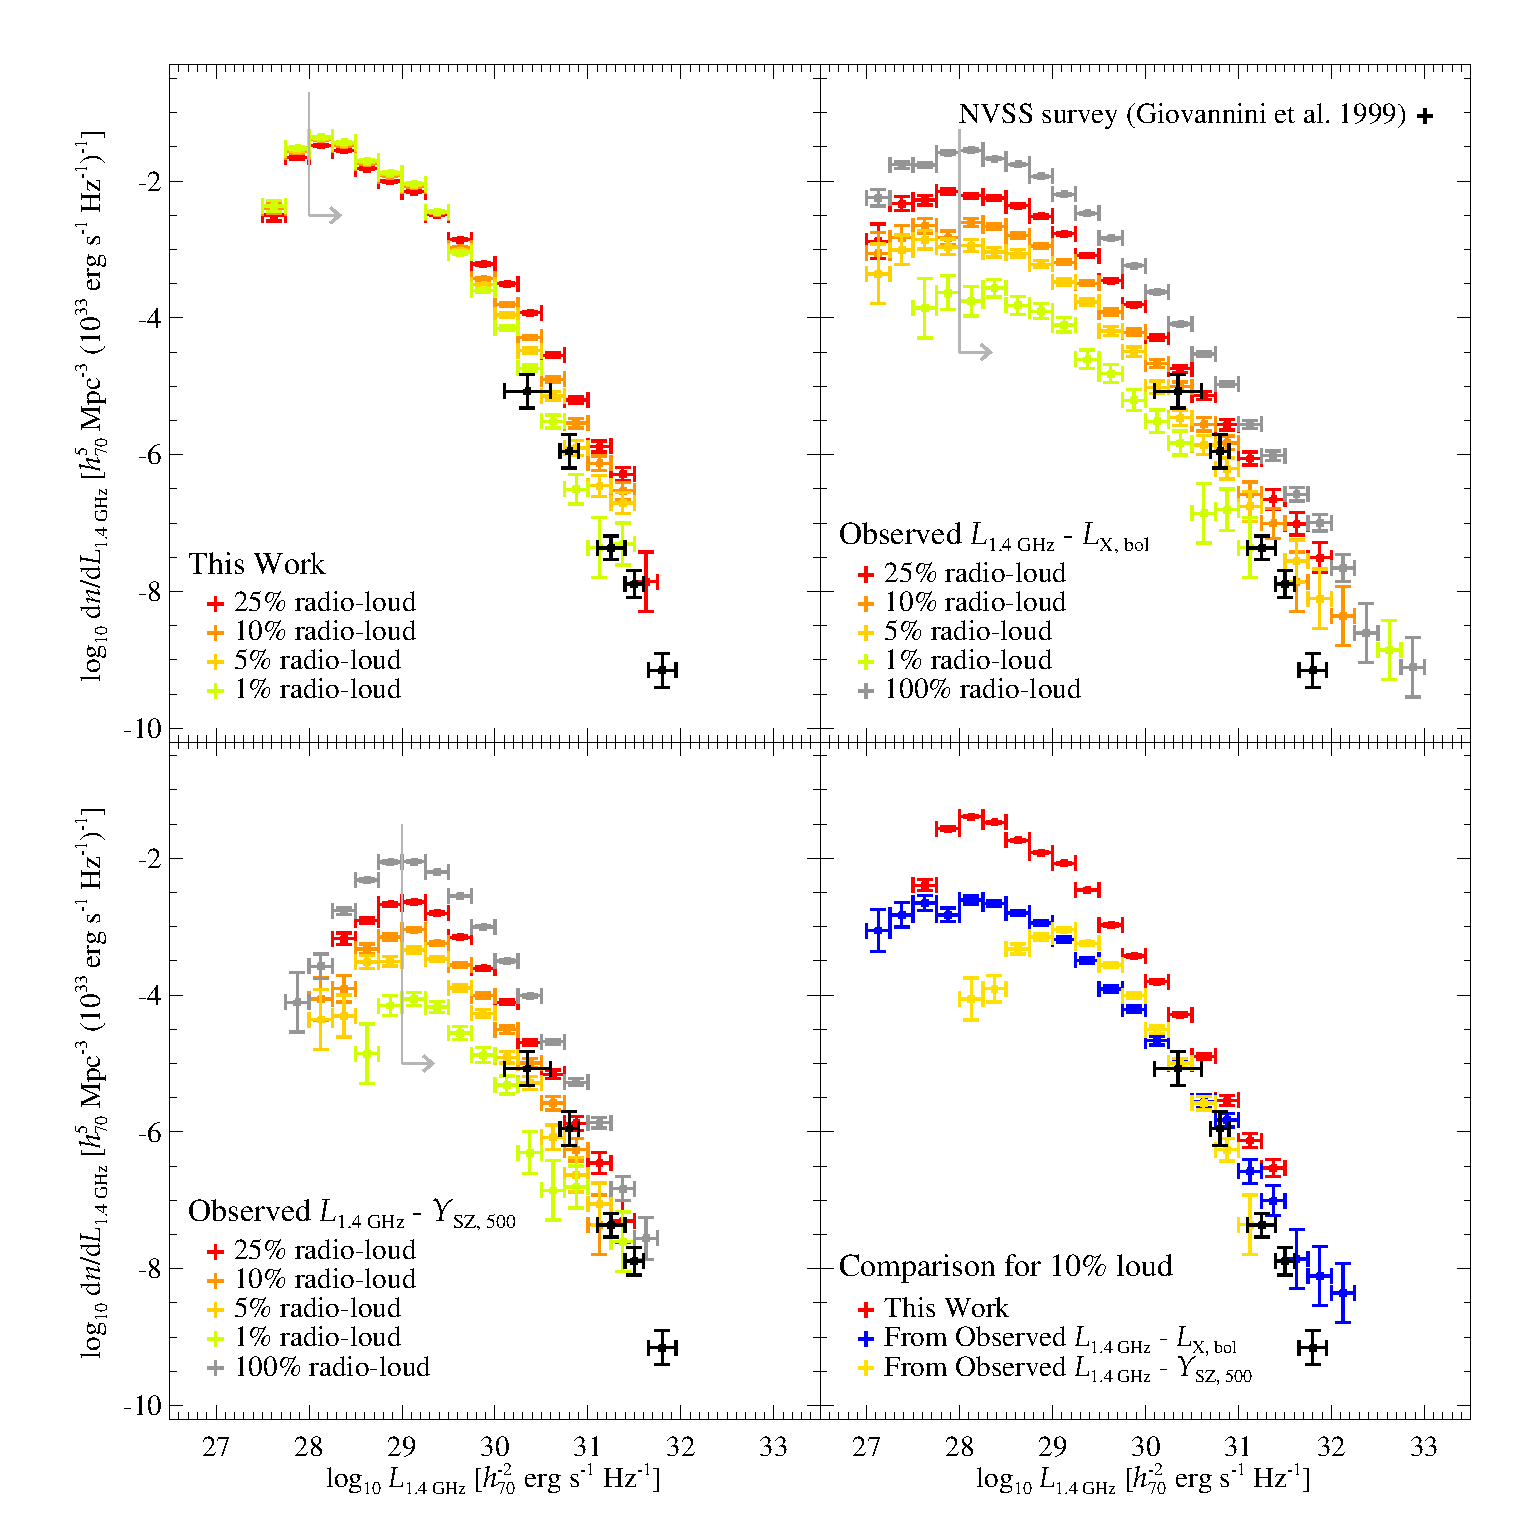
\includegraphics[width=0.85\textwidth]{figures/RLFs_1.4.eps}
\caption{Radio Luminosity Function at 1.4~GHz. The top left plot shows the prediction of our final CR model (see main text for the details of the chosen parameters) for different percent of radio-loud clusters, 25\%, 10\%, 5\% and 1\%. The top right plot shows the result obtained applying the observed $L_{1.4~\rmn{GHz}}-L_{\rm{X,bol}}$ directly to the MultiDark mass function at  $z = 0.2$, using the $L_{\rm{X,bol}}$ of each halos as obtained from our phenomenological model, for different percent of radio-loud clusters. The bottom left plot shows the result obtained applying the observed $L_{1.4~\rmn{GHz}}-Y_{\rm{SZ}, 500}$ directly to the MultiDark mass function at  $z = 0.2$,  using the $Y_{\rm{SZ}, 500}$ of each halos as obtained from our phenomenological model, for different percent of radio-loud clusters. The bottom right plot shows the comparison between the three approaches for 10\% of radio-loud clusters. The NVSS survey RLF \citep{1999NewA....4..141G} is also shown in all plots. The horizontal error bars represent the mass bins while the vertical error bars are Poissonian uncertainties. The light gray line with arrow shows the value above which the the RLF can be considered not affected by the low-luminosity decrease tail produced by our adopted mass cut (see Section~\ref{sec:2}) and the scatter in the halo luminosities.}
\label{fig:RLF_1.4}
\end{figure*}

In Figure~\ref{fig:RLF_1.4}, we show the RLF obtained from our final CR model and we compare it with observational results. Also in this case, as for the X-ray emission, the RLF is completely determined by the cluster mass function and the radio luminosity-to-mass relation, through $L_{1.4~\rmn{GHz}}-L_{ \rm{X,bol}}$ or $L_{1.4~\rmn{GHz}}-Y_{\rm{SZ}}$. Here the only additional uncertainty is the fraction of radio-loud clusters. Therefore, in Figure~\ref{fig:RLF_1.4}, we also show the ``true'' RLFs obtained applying  the $L_{1.4~\rmn{GHz}}-L_{\rm{X,bol}}$ and $L_{1.4~\rmn{GHz}}-Y_{\rm{SZ}}$ relations to our MultiDark $z = 0.2$ snapshot using their $L_{\rm{X,bol}}$ and $Y_{\rm{SZ}, 500}$, as obtained from our phenomenological model, respectively. Pay attention that this is done using \emph{only} the halos defined as radio-loud clusters, not all of them, and we show the cases for 100\%, 25\%, 10\%, 5\% and 1\% radio-loud clusters. As clear from Figure~\ref{fig:RLF_1.4}, this is different from what is obtained with our model, where a fraction of radio-loud cluster is indeed defined, but the radio-quiet population is also contributing to the RLF. Additionally, in Appendix~\ref{app:D}, we make an attempt to construct a RLF from existing X-ray flux-limited radio surveys. There exist two such studies, the cluster radio survey done with the National Radio Astronomy Observatory (NRAO) VLA sky survey (NVSS) at $1.4$~GHz of \cite{1999NewA....4..141G} and the one done with the Giant Metrewave Radio Telescope (GMRT) at $610$~MHz by \cite{VenturiGMRT_1,VenturiGMRT_2}. For the latter, one can also construct a RLF at 1.4~GHz using the corresponding RHs follow-up measurements. The fractions of radio-loud clusters, corrected for the incompleteness, are about 8\%, 26\% and 27\% for the NVSS 1.4~GHz, GMRT 610~MHz and GMRT 1.4~GHz samples respectively. The most problematic aspect in obtaining these RLFs, apart the small samples, is the calculation of a meaningful flux limit and therefore, as explained in Appendix~\ref{app:D}, we finally use the 1.4~GHz NVSS RLF (with a median redshift of $z \approx 0.18$) as reference for our comparisons with observation. We want to stress that the observational RLF determination, as explained in Appendix~\ref{app:D}, is extremely uncertain. Indeed, the very different percent of radio-loud clusters found in different studies is an indicator of this. 

\begin{figure*}[hbt!]
\centering
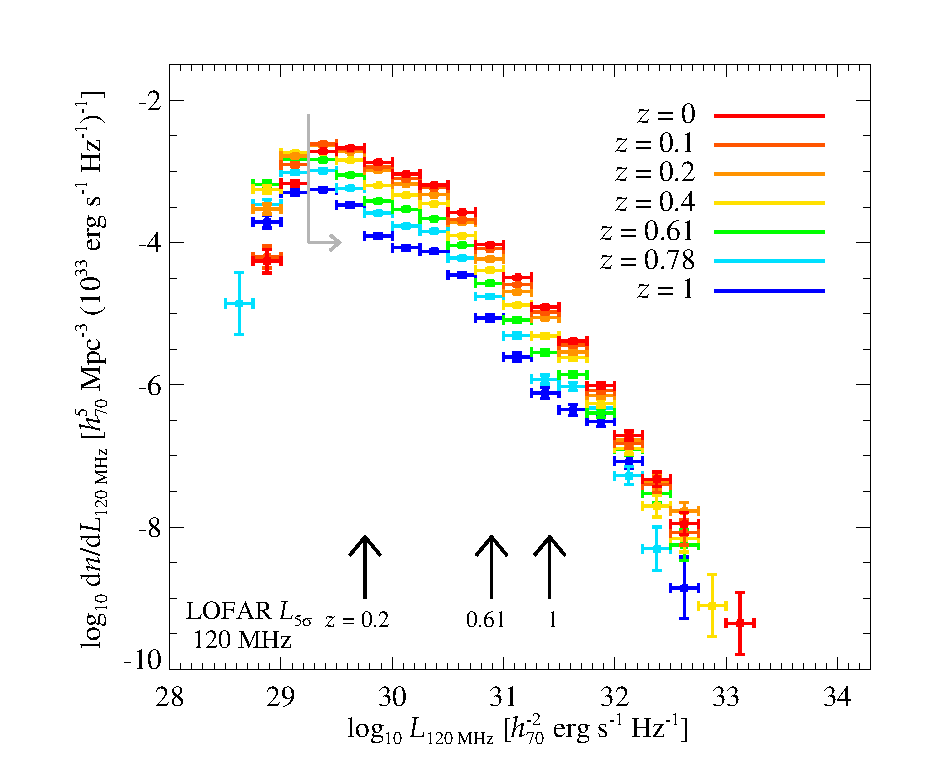
\includegraphics[width=0.5\textwidth,height=0.305\textheight]{figures/RLF_LOFAR.eps}
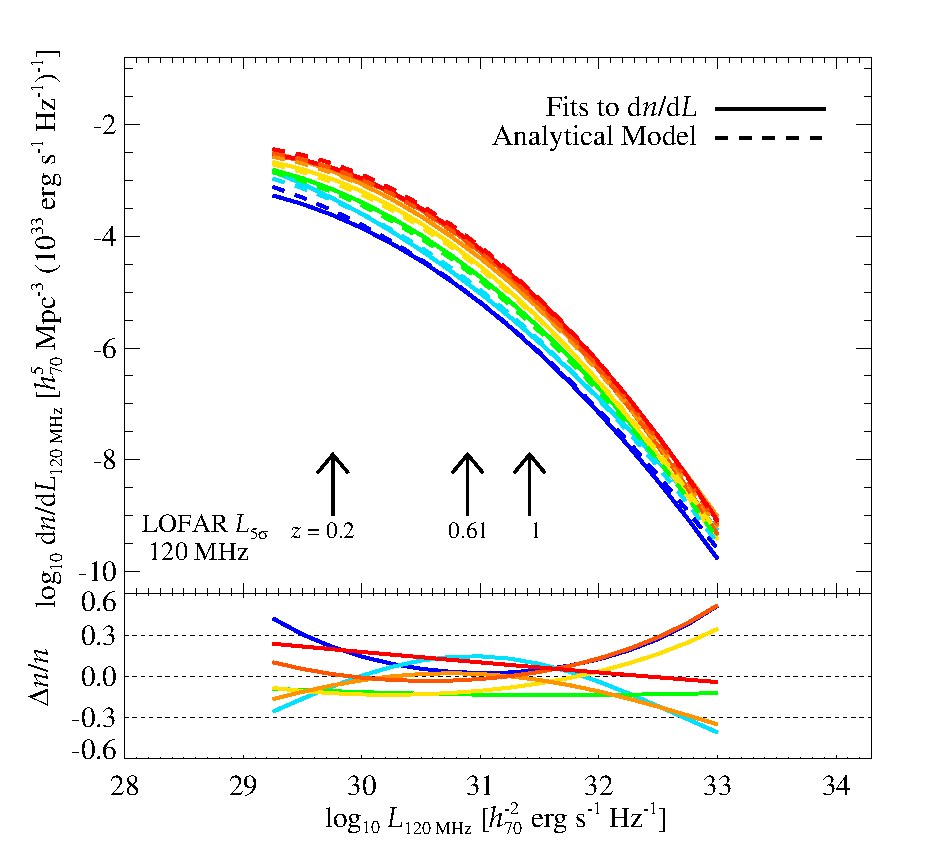
\includegraphics[width=0.47\textwidth,height=0.3\textheight]{figures/RLF_LOFAR_analytical_1.eps}
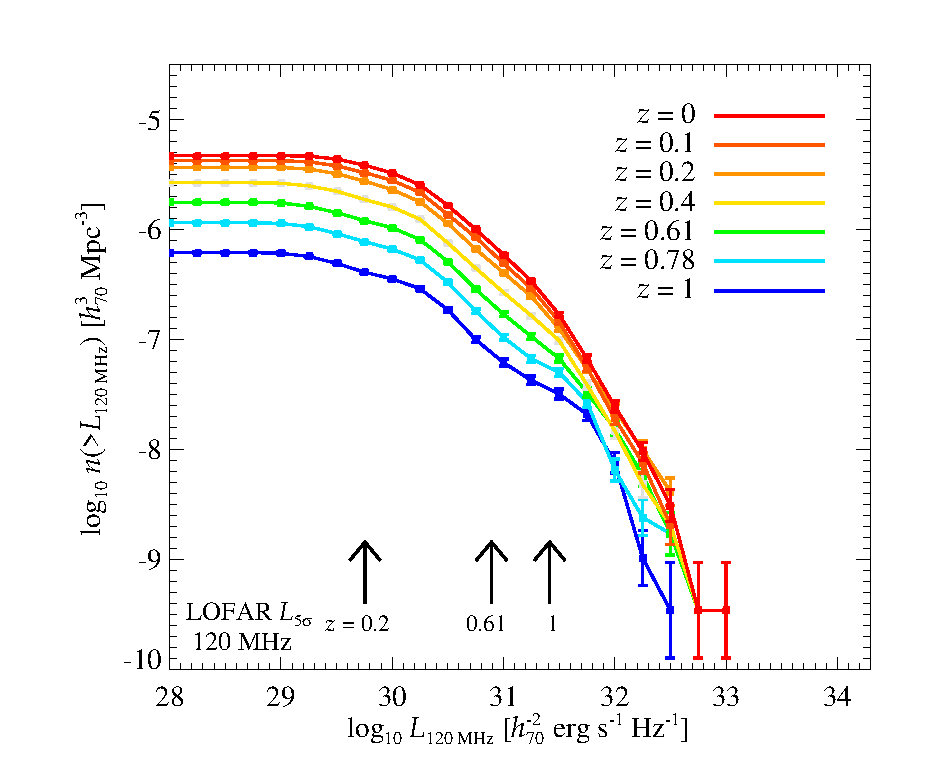
\includegraphics[width=0.5\textwidth,height=0.305\textheight]{figures/CumDensityL_LOFAR.eps}
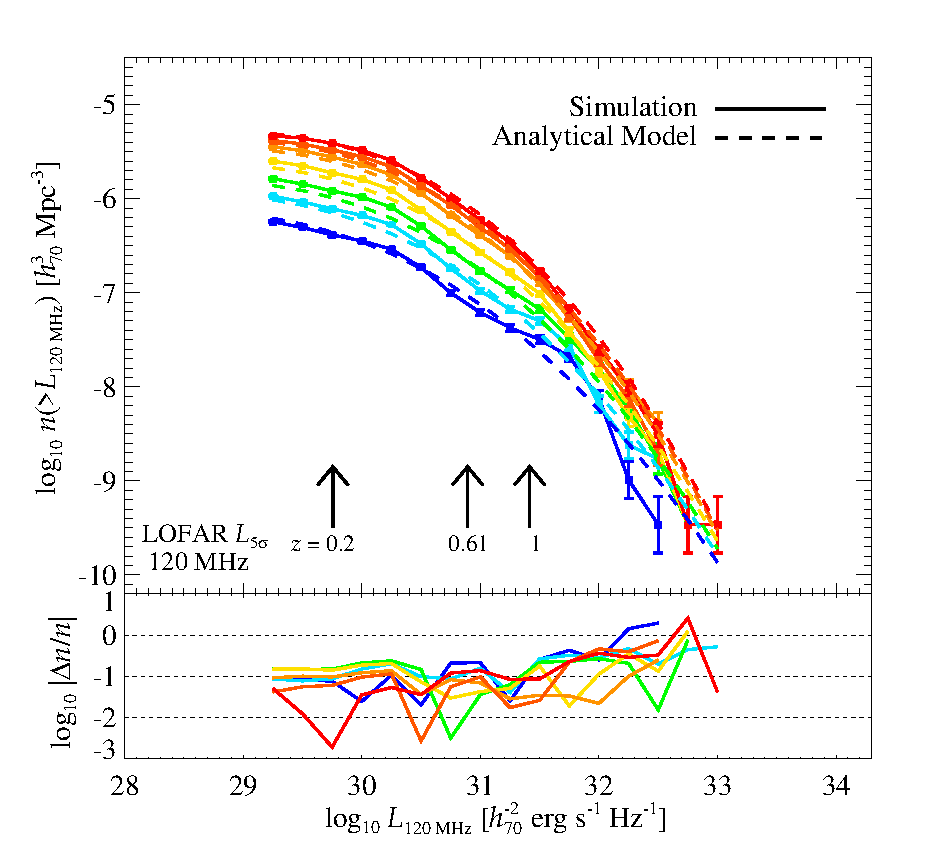
\includegraphics[width=0.47\textwidth,height=0.3\textheight]{figures/CumDensityL_LOFAR_1.eps}
\caption{Radio luminosity function (top left plot) and cumulative number density (bottom left plot) at the different MultiDark samples of Table~1 at 120~MHz for the model realization described in Section~\ref{sec:4} with 10\% fraction of radio-loud clusters. By fitting the RLF with a 2-order polynomial function and modeling the 3 free parameters with respect to the redshift evolution, we obtain an analytical model for $n(L,z)$ (see main text for details). The right plots show the comparison of the RLF fits (top) and the cumulative number density of the MultiDark samples (bottom) with the result obtained with the analytical model. The bottom panels of these two plots show the relative differences as $\Delta n / n = (n_{\rmn{analytical}} - n_{\rmn{fit}})/n_{\rmn{fit}}$ and $(\Delta n / \sigma_{n})/N = ((n_{\rmn{analytical}} - n_{\rmn{simulation}})/\sigma_{n,\rmn{simulation}})/N$, where $N$ is the total number of objects in each bin. Additionally shown is the LOFAR Tier~1 flux limit of $F_{\rm{limi},5\sigma}=0.5$~mJy \citep{2012JApA..tmp...34R} converted in luminosity limit at a given redshift. The light gray line with arrow in the bottom left plot shows the value above which the the RLF can be considered not affected by the low-luminosity decrease tail produced by our adopted mass cut (see Section~\ref{sec:2}) and the scatter in the halo luminosities.}
\label{fig:RLF_120}
\end{figure*}

Looking in detail to Figure~\ref{fig:RLF_1.4}, we can see that there is a good agreement between the NVSS survey result and both our RLF and the ``true'' RLFs, particularly for fraction of radio-loud clusters between 10\% and 1\%. The larger discrepancy seems to be present in the RLF obtained from the $L_{1.4~\rmn{GHz}}-L_{\rm{X,bol}}$ where the  observed relation scatter is producing a high luminosity tail of objects contradicting the NVSS result. On the other side, the RLF obtained from the $L_{1.4~\rmn{GHz}}-Y_{\rm{SZ}}$ seems the one better matching the NVSS result. We warn the reader that both of these facts may however be artifacts due to the interplay of the two relation scatter and the still small statistic of our MultiDark $z = 0.2$ snapshot at very high masses. Note also how important is the effect on the resulting RLF of having different scatter values. We do not give too much weight to these comparisons because of the uncertain determination at this stage of the observational RLF as well as of the observational $L_{1.4~\rmn{GHz}}-L_{\rmn{X,bol}}$ and $L_{1.4~\rmn{GHz}}-Y_{\rm{SZ}}$ scaling relations. Figure~\ref{fig:RLF_1.4} shows that it seems difficult that we will be able to firmly discriminate between different scenarios at high radio luminosities (or masses). Indeed, the bottom right plot of Figure~\ref{fig:RLF_1.4}, where we compare our RLF and the ``true'' RLFs at 10\% radio-loud cluster fraction, suggests that the lower luminosity (mass) clusters will be the most powerful way to disentangle between different models. Therefore, it is clear the key role of the upcoming LOFAR cluster survey for which we present predictions in the next section. Finally, note the clear low-luminosity decrease in the RLFs that is an artifact due to the adopted mass cut, below which therefore there are no clusters in our sample (see Section~\ref{sec:2}), and the scatter in the halo luminosities. 

%%%%%%%%%%%%%%%%%%%%%%%%%%%%%%%%%%%%%%%%%%%%%%%%%%%%%%%%%%%%%%%%%%%
%%%%%%%%%%%%%%%%%%%%%%%%%%%%%%%%%%%%%%%%%%%%%%%%%%%%%%%%%%%%%%%%%%%
\section{Predictions for LOFAR}
\label{sec:5}

In Figure~\ref{fig:RLF_120}, we show the predictions obtained with a particular realization of our model (explained in the previous section, with 10\% of radio-loud clusters) at 120~MHz. We show both the RLF (top left plot) and the cumulative number density (bottom left plot) at the different MultiDark snapshots of Table~1. Additionally shown is the expected LOFAR Tier~1 flux limit of $F_{\rm{limi},5\sigma}=0.5$~mJy \citep{2012JApA..tmp...34R} converted in luminosity limit at a given redshift. The figures show that the LOFAR survey should be able to determine the 120~MHz RLF properties in a very broad range of luminosities. Particularly, it should permit a robust determination of the number of clusters hosting RHs at a given luminosity. This will be extremely helpful in determining the parameter values in our model, and eventually in elucidating the RH generation mechanism.

In order to make a more quantitative prediction, we construct an analytical model to describe $\rmn{d}n/\rmn{d}L$. We fit the 120~MHz RLF at different redshift as a 2-order polynomial function in the form of $\log_{10} \rmn{d}n/\rmn{d}L_{120~\rmn{MHz}} = A_{1} + A_{2}~\log_{10} L_{120~\rmn{MHz}} + A_{3}~(\log_{10} L_{120~\rmn{MHz}})^{2}$, where only luminosities higher then $\log_{10} L_{120~\rmn{120MHz}} \geq 29.25$ are used in order to exclude the artificial low luminosity decrease. We then obtain an analytical form for the dependence of the three parameters $A_{i}$ with respect to the redshift as $A_{i} = A_{i,0} + A_{i,1}~(1+z)$.\footnote[15]{The values of these parameters are $A_{1,0} = -436.79$, $A_{1,1} = 109.75$, $B_{1,0} = 29.68$, $B_{1,1} = -7.17$, $C_{1,0} = -0.51$ and $C_{1,1}$ = 0.12.} In the right plots of Figure~\ref{fig:RLF_120}, we compare the RLF fits to the result obtained with the so-derived analytical model (top) and the cumulative number density with the one obtained integrating the analytical model (bottom). The results obtained with this analytical model well compare with the prediction at a given redshift showing a significant deviation only at very high luminosities, and at very low luminosities for the highest considered redshifts, where however the small statistic significantly affects the comparison. 

This analytical model describing $n(L,z)$ can therefore be used to calculate the total cumulative number of RHs in the sky above a given flux limit as shown in Figure~\ref{fig:RLF_120_flux}. We show the result for the particular realization of our model described in the previous section with 10\% fraction of radio-loud clusters (black solid think line; only luminosities above $\log_{10} L_{120~\rmn{120MHz}} \geq 29.25$ are integrated). The total prediction is obtained integrating from redshift 0 up to 2, because using the MultiDark snapshot at $z = 1.87$ we verified that only about 70 halos survive our mass cut and only a handful of them would be detectable. We also show how the total result builds up in different redshift bins. We contrast this with the RH total cumulative number obtained using \emph{only} the 10\% radio-loud clusters (blue solid think line; this is done constructing the corresponding RLF and repeating the above steps to construct an analytical model, where only luminosities above $\log_{10} L_{120~\rmn{120MHz}} \geq 30.75$ are integrated). We additionally shown the two total results scaled down by a $50\%$ to roughly mimic an eventual RH redshift evolution as a consequence of a higher inverse Compton energy loss on the CMB for higher redshift (\citealp{2002A&A...396...83E}; this is somehow conservative as most of our cluster magnetic fields are comparable or higher than the CMB magnetic field). 

\begin{figure}[hbt!]
\centering
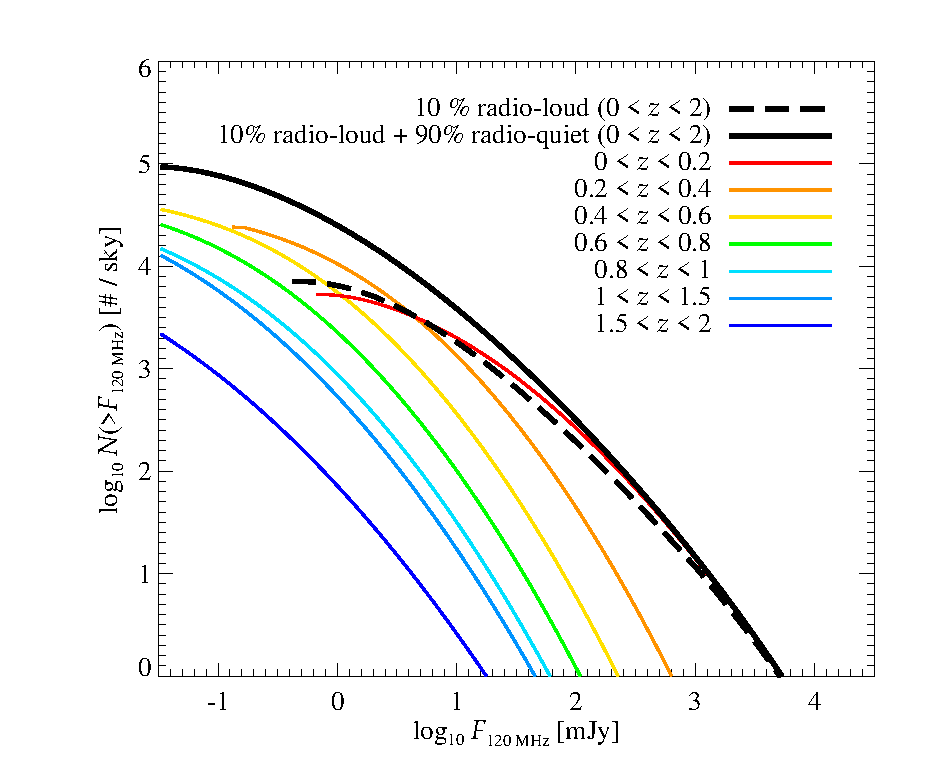
\includegraphics[width=0.5\textwidth]{figures/RLF_LOFAR_flux.eps}
\caption{Cumulative number of RHs above a certain flux limit in all the sky at 120~MHz. We show the result of the model realization described in Section~\ref{sec:4} with 10\% fraction of radio-loud clusters (black lines) and the result obtained using only the 10\% radio-loud clusters (blue lines). We additionally shown the two predictions scaled by 50\% as to roughly mimic a RH redshift evolution as a consequence of a higher inverse Compton energy loss on the CMB for higher redshift \citep{2002A&A...396...83E}. The upper limit of the integration is $z = 2$ as above this redshift there are no clusters surviving our mass cut in the MultiDark simulation. Additionally shown at 1~mJy is the $10\sigma$ flux limit of LOFAR at 120~MHz. Note that the total number of detectable RHs would be dramatically reduced in the presence of a break in the model at some low mass-scale, or some sort of mass-dependence in the model parameters, causing a lowering of the RH luminosities at low masses. Both effects are for the time being not considered as the current information do not permit to make any reliable assumption in this sense. See main text for details.
}
\label{fig:RLF_120_flux}
\end{figure}

Figure~\ref{fig:RLF_120_flux} shows that about $10^4-10^5$ clusters hosting RHs should be detectable above 1~mJy (approximately corresponding to the LOFAR 10$\sigma$ flux limit at 120~MHz for).\footnote[16]{Note that the LOFAR Tier~1 sky coverage is about half of the total sky.} However, as clear from the figure, the precise number is strongly dependent on the underling assumptions. There are two main uncertainties in our model: the fraction of radio-loud to radio-quiet clusters and the corresponding relative normalization (which in turn is the result of the interplay of the $\gamma_{\rmn{th}}$, $B_{0}$, $\alpha_{B}$, $g_{\rmn{CR}}$, and therefore $X_{CR}$, parameters). The first point is relevant only at medium-high luminosities, as can be seen for the 1.4~GHz RLFs in Figure~\ref{fig:RLF_120}, and therefore would not dramatically impact the total number of detectable clusters above the LOFAR flux limit because this is dominated by the low luminosities. We asses the second point by comparing the total result of our model (black) with the RLF obtained only from the radio-loud population (blue); their difference virtually shows the uncertainty in the modeling. Despite the difference between these two models is almost an order of magnitude at the LOFAR flux limit, the total number of detectable RHs is still expected to by very high. This is mainly due to neglecting an eventual mass-dependence in the model parameters and, more importantly, to the assumption that the model holds down to masses of about $M_{200}\approx1.4\times10^{14}$~$h_{70}^{-1}$~M$_{\odot}$ without any break. In fact, looking at the radio-to-X-ray and radio-to-SZ scaling relations of Figure~\ref{fig:PLSZ}, we can see that most of the RHs in our sample, also for the radio-loud population, lie at low masses and therefore at low luminosities unproved by current observations. The presence of a break at some low mass-scale, or some sort of mass-dependence in the model parameters, causing a lowering of the RH luminosities, would eventually result in a dramatically reduced number of total detectable RHs. This would be more in agreement with recent predictions of a few to hundreds observable RHs (see e.g.~\citealp{2010A&A...509A..68C} and \citealp{2011arXiv1110.2786S}), while \cite{2002A&A...396...83E} also found that thousands of RHs would be detectable by future surveys. However, the current information do not permit to make any reliable assumption in this sense and we indeed have to wait the future LOFAR results to shed light on these fundamental issues. 


%%%%%%%%%%%%%%%%%%%%%%%%%%%%%%%%%%%%%%%%%%%%%%%%%%%%%%%%%%%%%%%%%%%
%%%%%%%%%%%%%%%%%%%%%%%%%%%%%%%%%%%%%%%%%%%%%%%%%%%%%%%%%%%%%%%%%%%
\section{Discussion and Conclusions}
\label{sec:6}
BLA BLA BLA\\


%%%%%%%%%%%%%%%%%%%%%%%%%%%%%%%%%%%%%%%%%%%%%%%%%%%%%%%%%%%%%%%%%%%
%%%%%%%%%%%%%%%%%%%%%%%%%%%%%%%%%%%%%%%%%%%%%%%%%%%%%%%%%%%%%%%%%%%
\begin{acknowledgements}
We would like to thank Anders Pinzke for his invaluable help with the formulae and for many useful discussions. We also thanks Gustavo Yepes, Jos\'e Alberto Rubi\~no, Frazer Pearce, Andrey Kravtsov, Harald Ebeling, Miguel-Angel Perez Torres and Adam Mantz for the useful discussions and advices. We would also like to thank Matteo Murgia for kindly providing the radio surface brightness of Ophiuchucs and Abell~2163, and Wolfgang Reich for providing the radio map of Coma. {\bf Thanks MultiDark database guys, etcetera}.
BLA BLA BLA\\ 
F.~Z.~acknowledges the CSIC financial support as a JAE-Predoc grant of the program ``Junta para la Ampliaci\'on de Estudios'' co-financed by the FSE.
\end{acknowledgements}


%%%%%%%%%%%%%%%%%%%%%%%%%%%%%%%%%%%%%%%%%%%%%%%%%%%%%%%%%%%%%%%%%%%
%%%%%%%%%%%%%%%%%%%%%%%%%%%%%%%%%%%%%%%%%%%%%%%%%%%%%%%%%%%%%%%%%%%
\begin{appendix}
\section{Radio Emission Calculation}
\label{app:A}

We explicitly write down here $A_{\nu}$ for the synchrotron radio luminosity calculation of Equation~(\ref{eq:surface_brightness_1}):

\begin{equation}
A_{\nu} = A_{\rm{E_{synch}}} \frac{16^{2-\alpha_{\rm{e}}}\sigma_{\rm{pp}}m_{\rm{e}}c^{2}}{(\alpha_{\rm{e}}-2)\sigma_{\rm{T}}\epsilon_{B_{\rm{C}}}m_{\rm{p}}}\left(\frac{m_{\rm{p}}
}{m_{\rm{e}}}\right)^{\alpha_{\rm{e}}-2} \left(\frac{m_{\rm{e}}c^{2}}{\rmn{GeV}}\right)^{\alpha_{\rm{e}}-1}
\end{equation}

with:

\begin{equation}
A_{\rm{E_{synch}}} = \frac{\sqrt{3\pi}}{32\pi}\frac{B_{\rm{c}}e^{3}}{m_{\rm{e}}c^{2}}\frac{\alpha_{\rm{e}}+\frac{7}{3}}{\alpha_{\rm{e}}+1}\frac{\Gamma\left(\frac{3\alpha_{\rm{e}}-1}{12}\right)\Gamma\left(\frac{3\alpha_{\rm{e}}+7}{12}\right)\Gamma\left(\frac{\alpha_{\rm{e}}+5}{4}\right)}{\Gamma\left(\frac{\alpha_{\rm{e}}+7}{4}\right)}
\end{equation}

where $\alpha_{\rm{e}}=\alpha+1$ and $\Gamma$ is the Gamma-function \citep{1965hmfw.book.....A}. $A_{\rm{E_{synch}}}$ is expressed in erg, and $A_{\nu}$ is expressed in erg~cm$^{3}$~g$^{-1}$~sr$^{-1}$. 
%The dimension of $A_{\rm{E_{synch}}}$ is [erg] if the electron charge $e$ is expressed in [ues], the electron mass $m_{\rm{e}}$ in [g], the speed of light $c$ in [cm/s] and the critical magnetic field value $B_{\rm{c}}$ in [G]. The dimension of $A_{\nu}$ is [erg~cm$^{3}$~g$^{-1}$~sr$^{-1}$] if the effective inelastic cross-section for proton-proton interactions $\sigma_{\rm{pp}} = 32~(0.96+\rm{e}^{4.42-2.4\alpha})$ and the Thomson cross-section $\sigma_{\rm{T}}$ are expressed in [mbarn], the first $m_{\rm{e}}$ in [g], the first $c$ in [cm/s], $B_{\rm{c}}$ of $\epsilon_{B_{\rm{C}}}$ is expressed in [G] and $m_{\rm{p}}$ in [g]. 
%Pay attention that here the $B_{C}$ value must be expressed in [G] to get the correct final units while in the main text it is expressed in [$\mu$G] because there it cancels out with the other magnetic field values.  

The generalization of $A_{\nu}$ to three CR spectral indexes and the inclusion of the maximum CR acceleration efficiency parameter $g_{\rm{CR}}$, following \cite{2010MNRAS.409..449P}, would give the new $A_{\nu, final}$:

\begin{equation}
A_{\nu, \rm{final}} = g_{\rm{CR}} \Sigma_{i=1}^{3} \Delta_{i} A_{\nu,i}
\end{equation}

where the sum is over the three CR spectral indexes $\alpha_{i}=(2.55,2.3,2.15)$ with the corresponding factors $\Delta_{i} = (0.767, 0.143, 0.0975)$ found by Pinzke and Pfrommer in their simulations. At the same time the extension must include the factor $(\epsilon_{\rm{B}}(R)/\epsilon_{B_{\rm{c}}})^{(\alpha_{i}-2)/4}$ of the luminosity calculation practically changing $j_{\nu}(R)=A_{\nu}\tilde{S}_{\nu}(R)$ into: 

\begin{eqnarray}
j_{\nu,\rm{final}}(R) & = &g_{\rm{CR}} C(R) \rho_{\rm{gas}}(R) \frac{\epsilon_{\rm{B}}(R)}{\epsilon_{\rm{B}}(R)+\epsilon_{\rm{CMB}}} \nonumber \\
& \times & \Sigma_{i=1}^{3} \Delta_{i} A_{\nu,i} \left( \frac{\epsilon_{\rm{B}}(R)}{\epsilon_{B_{\rm{c}}}} \right)^{\frac{\alpha_{i}-2}{4}}  \quad .
\end{eqnarray}
 
\end{appendix}

%%%%%%%%%%%%%%%%%%%%%%%%%%%%%%%%%%%%%%%%%%%%%%%%%%%%%%%%%%%%%%%%%%%
%%%%%%%%%%%%%%%%%%%%%%%%%%%%%%%%%%%%%%%%%%%%%%%%%%%%%%%%%%%%%%%%%%%
\begin{appendix}
\section{Cosmic Rays Modeling Details}
\label{app:B}

In order to make some comparisons between $C_{\rm{simple}}$ and $C_{\rm{transport}}$ we take as reference cases the NCCC Coma and the CCC Perseus. While for Coma the $\beta$-profile of Equation~(\ref{eq:beta_profile}) is a good approximation, and we take the \cite{1992A&A...259L..31B} profile for it, for Perseus we need a double-$\beta$ profile. We adopt both the approximation $P(R)/P_{0}=n_{\rm{e}}(R)/n_{0}$, with $n_{\rm{e}}(R)$ the double-$\beta$ profile of \cite{2003ApJ...590..225C}, and the proper Perseus pressure profile as in Section~\ref{sec:3} (for Perseus, we take $R_{\rm{c}}$ to be equal to the outer double-$\beta$ profile core radius and we fix $\beta_{\rm{cl}}=0.8$). Note that the \cite{2011A&A...527A..99E} formalism is exact only for the approximation $P(R)/P_{0}=n_{\rm{e}}(R)/n_{0}$ and in the case of a $\beta$-profile. There is not an exact analytical solution for the case of a double-$\beta$ profile: one should use a numerical solution. In this work, we make different choices for $P(R)/P_{0}$, and we construct a model that has to be applied to all the halos of our sample. We therefore do not try to solve numerically each case. We instead just adopt the \cite{2011A&A...527A..99E} formalism as a good approximation. The relevant parameters are $\gamma_{\rm{tu}}$, the exponential factor of Equation~(\ref{eq:Ctransport}), and the two radius $R_{\pm}$ that in general are very small/large so that the detail of $P(R)/P_{0}$ does not affect them critically. Indeed, we are dominated by other uncertainties, e.g. the assumption that the characteristic radius at which the turbulence is injected is the cluster core radius, so with this approach we are confident that we capture the main CR transport effects on the overall cluster properties despite the approximation.

\begin{figure*}[hbt!]
\centering
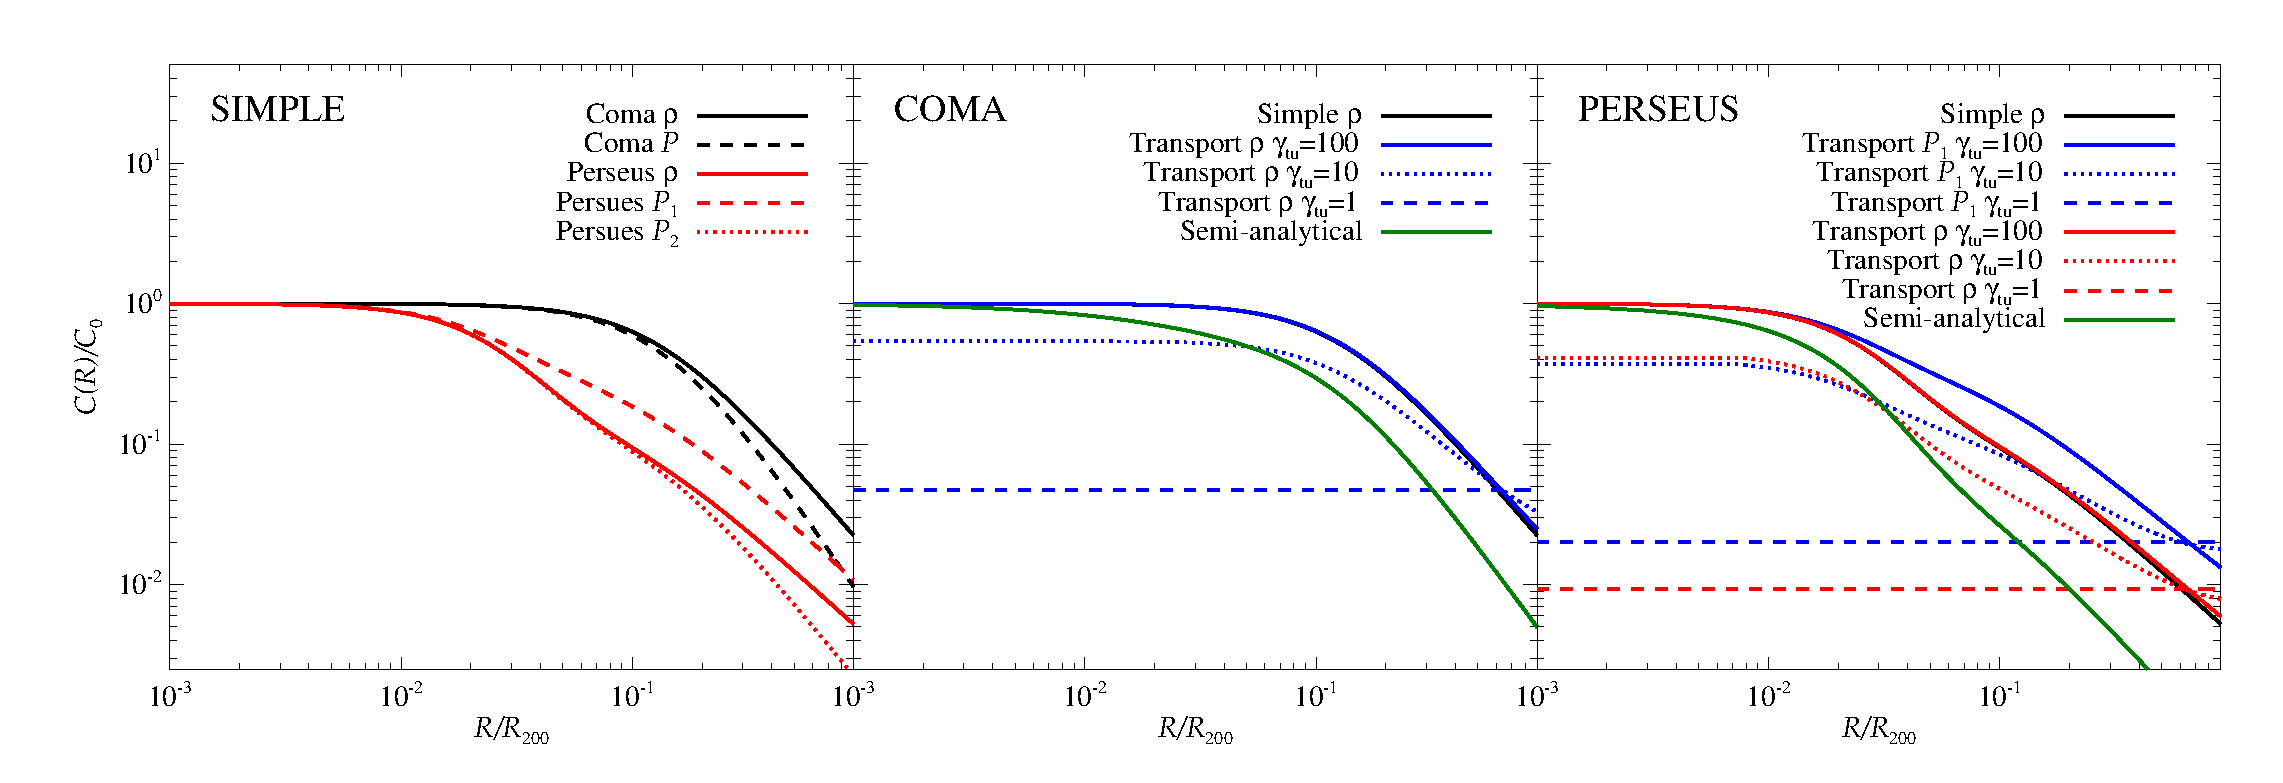
\includegraphics[width=0.99\textwidth]{figures/CR_profiles_simple_comparison.eps}
\caption{Comparison of different CR profiles. The left plot shows $C_{\rm{simple}}$ for the Coma and Perseus cases both neglecting the temperature dependence ($\rho$) and considering it ($P$). The temperature profile of Coma has been modified so that it follows the characteristic decline toward the cluster periphery \citep{2007MNRAS.378..385P,2010MNRAS.409..449P}. Perseus is a CCC and it is characterized by a central dip in the temperature profile which may importantly affect the final CR profile, so we adopt the temperature profile as given in \citep{2004A&A...413...17P} ($P_{1}$). We also show the case where we only apply the characteristic decline toward the cluster periphery ($P_{2}$). The other two right plots show the \emph{transport} case of Coma and Perseus for different values of $\gamma_{\rm{tu}}$ in comparison with the \emph{simple} case. Additionally shown is the result in case of $C(R)=C_{\rm{semi-analytical}}(R)=\tilde{C}(R)\rho_{\rm{gas}}(R)/m_{\rm{p}}$ where $\tilde{C}(R)$ is the mass-dependent universal normalization CR profile found in cosmological simulations of \cite{2010MNRAS.409..449P}. The \emph{simple} and \emph{semi-analytical} profiles are normalized at $C_{0}=C(0)$. The transport cases are normalized at $C_{0}=C(0,\gamma_{\rm{tu}}=100)$, where we fix the CR populations to have a constant total CR number as in Equation~(36) of \cite{2011A&A...527A..99E} integrating up $R_{200}$. We adopt $\alpha=2.3$.}
\label{fig:simpleVStransport}
\end{figure*}

We show the comparison between $C_{\rm{simple}}$ and $C_{\rm{transport}}$ in Figure~\ref{fig:simpleVStransport}, where we also show the result in case $C(R)=C_{\rm{semi-analytical}}(R)=\tilde{C}(R)\rho_{\rm{\rm{gas}}}(R)/m_{\rm{p}}$ where $\tilde{C}(R)$ is the mass-dependent universal normalization CR profile found in cosmological simulations of \cite{2010MNRAS.409..449P}. As expected, the CR profile driven by simulations is characterized by a more centrally peaked profile with respect to the analytical case. Note also the much more centrally peaked profile of Perseus with respect to Coma, which reflects their CCC and NCCC classification respectively, and the impact that have neglecting the temperature dependence in the Perseus case. Finally, the anticipated effect of varying the turbulent cluster state by means of $\gamma_{\rm{tu}}$ can be clearly appreciated.

We want to generalize the En{\ss}lin approach to our GNFW gas profiles obtained in Section~\ref{sec:2.2} and merge the \cite{2011A&A...527A..99E} analytical approach with the $\tilde{C}$ universal CR normalization obtained from simulations. Also in this case there is not an exact solution for the \cite{2011A&A...527A..99E} treatment of the problem. In fact, when trying to solve it analytically, one ends up with a 5-order equation. It is not practical to solve numerically such equation, and at the same time to discharge the unphysical solution, for our more than $10^4$ halos. For simplicity, we proceed with the approximation of using the \cite{2011A&A...527A..99E} formalism, after some modifications in order to adapt it to our case. In the case of taking just $P(R)/P_{0}=n_{\rm{e,GNFW}}(R)/n_{0}$, with $n_{\rm{e,GNFW}}$ the profile of Equation~(\ref{eq:gnfw}), there exist an exact solution following the \cite{2011A&A...527A..99E} treatment. Therefore, in order to qualitatively have an idea of how much is the error that we are making with the above described approach, in Figure~\ref{fig:REXexactVSfake} we compare the $C_{\rm{transport}}(R)$ of the GNFW exact solution and the approximate case where we use the \cite{2011A&A...527A..99E} formulae but just adopting $P(R)/P_{0}=n_{\rm{e,GNFW}}(R)/n_{0}$. In the second case, which after adding the temperature dependence will be our \emph{final} model, we fix $R_{-}=10^{-3}R/R_{200}$ to mimic the typical $R_{-}$ value of the exact solution, otherwise a unphysical step feature would appear around $10^{-2}R/R_{200}$. Note however that this modification does not change at all the model surface brightness and total luminosity. As clear from the figure, there is almost no appreciable difference between the two cases. 
%apart for the NCCC case with $\gamma_{\rm{tu}}=10$ where the approximated solution in the inner $<10^{-2}R/R_{200}$ is flat whether it is peaked for the exact solution. This is due to different values of $R_{-}$ between the two approaches, however the impact of such difference is in complex negligible. Note that this $<10^{-2}R/R_{200}$ flat behavior can also be seen in Figure~\ref{fig:simpleVStransport}, rightmost plot, where however it is not so evident because the double-$\beta$ profile used there is flatter than our CCC GNFW profile. 
This comparison makes us confident that the approximated approach strategy can be safely followed in order to derive a fully working model with the above described characteristics.

\begin{figure}[hbt!]
\centering
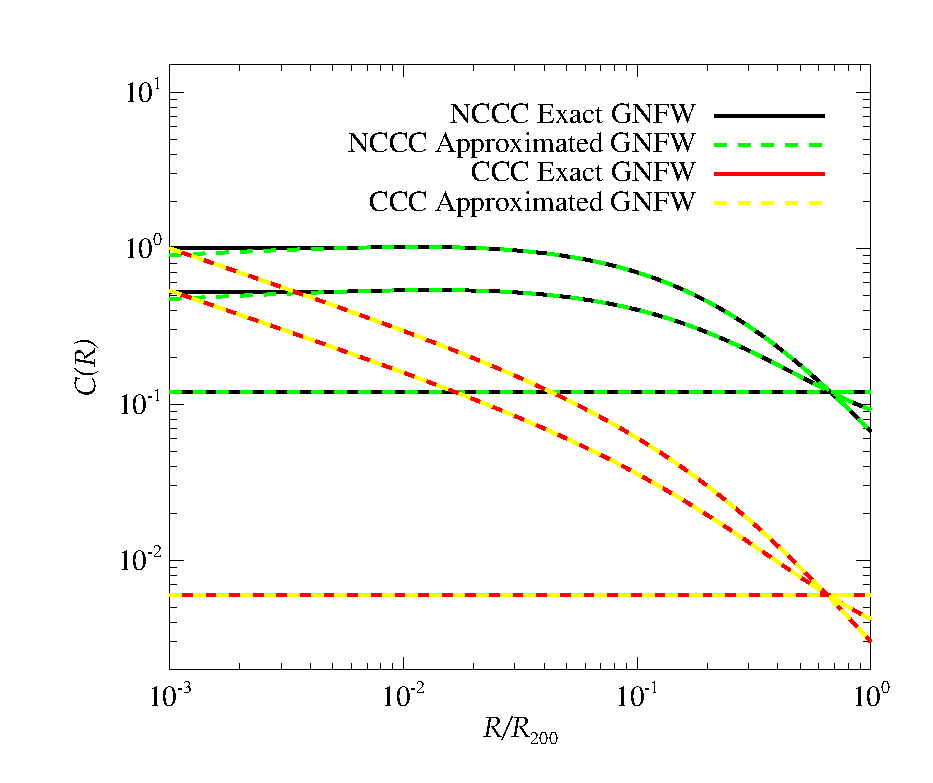
\includegraphics[width=0.5\textwidth]{figures/CR_profiles_REXexactVSfake.eps}
\caption{Comparison of $C_{\rm{transport}}(R)$ for the GNFW exact solution and the approximated case where we use the \cite{2011A&A...527A..99E} formulae with $P(R)/P_{0}=n_{\rm{e,GNFW}}(R)/n_{0}$. Both the NCCC and CCC case for the respective GNFW profiles derived in Section~\ref{sec:2.2} are shown. From top to bottom: $\gamma_{\rm{tu}}=100$, $\gamma_{\rm{tu}}=10$ and $\gamma_{\rm{tu}}=1$. The normalization is done at $C_{0}=C(0,\gamma_{\rm{tu}}=100)$ of the exact model where we fix the CR populations to have a constant total CR number as in Equation~(36) of \cite{2011A&A...527A..99E} integrating up $R_{200}$. Note that the $C(0,\gamma_{\rm{tu}}=100)$ value for the CCC case is identical between the exact and approximated model, while there is a small difference of about 9\% in the NCCC case .We adopt $\alpha=2.3$.}
\label{fig:REXexactVSfake}
\end{figure}

\end{appendix}

%%%%%%%%%%%%%%%%%%%%%%%%%%%%%%%%%%%%%%%%%%%%%%%%%%%%%%%%%%%%%%%%%%%
%%%%%%%%%%%%%%%%%%%%%%%%%%%%%%%%%%%%%%%%%%%%%%%%%%%%%%%%%%%%%%%%%%%
\begin{appendix}
\section{Gamma-ray Emission Calculation}
\label{app:C}

The gamma-ray flux above a certain energy $E_{\gamma}$ can be written as:

\begin{equation}
F_{\gamma} (E_{\gamma}) = \frac{1}{4\pi D^{2}} L_{\gamma} = 4\pi \int_{0}^{R_{500}} 2\pi S(R_{\perp}) R_{\perp} \rmn{d}R_{\perp}
\end{equation}

where $S(R_{\perp})$ is the surface brightness:

\begin{equation}
S(R_{\perp}) = 2 \int_{R_{\perp}}^{\infty} j_{\gamma}(R) \frac{R}{\sqrt{R^{2}-R_{\perp}^{2}}} \rmn{d}R
\end{equation}

with $ j_{\gamma}(R)=A_{\gamma}\tilde{S}_{\gamma}(R)$ and $\tilde{S}_{\gamma}(R)  =  C(R) \rho_{\rm{gas}}(R)$. The parameter $A_{\gamma}$ is \citep{2010MNRAS.409..449P}:

\begin{eqnarray}
A_{\gamma} = g_{\rm{CR}} D_{\gamma,\rm{break}} \frac{4 m_{\pi^{0}} c}{3 m_{\rm{p}}^{2}} \Sigma_{i=1}^{3} \Delta_{i} \frac{\sigma_{\rm{pp},i}}{\alpha_{i} \delta_{i}} \left( \frac{m_{\rm{p}}}{2 m_{\pi^{0}}} \right)^{\alpha_{i}} \times \nonumber \\
\times \left[ \beta_{x} \left( \frac{\alpha_{i}+1}{2\delta_{i}}, \frac{\alpha_{i}-1}{2\delta_{i}} \right) \right]_{x_{1}}^{x_{2}} 
\end{eqnarray}

where $x_{j}=\left[ 1 + \left( \frac{m_{\pi^{0}}c^2}{2E_{\gamma,j}} \right)^{2\sigma_{i}} \right]$, $\left[ \beta_{x}(a,b) \right]_{x_1}^{x_2} = \beta_{x_2}(a,b)-\beta_{x_1}(a,b)$ and $\beta$ denotes the incomplete Beta-function \citep{1965hmfw.book.....A}, and $\delta_{i}=0.14\alpha_{i}^{-1.6}+0.44$. The term $D_{\gamma, \rm{break}}=D_{\gamma}(E_{\gamma},E_{\gamma,\rm{break}})$ represent diffusive CR losses due to escaping protons from the cluster at the equivalent photon energy for the break $E_{\gamma, \rm{break}}$ (see \citealp{2010MNRAS.409..449P} for details). $A_{\gamma}$ is expressed in cm$^3$~s$^{-1}$~g$^{-1}$. 

%The factor A_{\gamma}$ has dimensions of [cm$^3$~s$^{-1}$~g$^{-1}$] if $E_{\gamma}$ enters in [GeV], $\sigma_{pp}$ is expressed in [cm$^{-2}$], $m_{\pi}^{0}$ and $m_{p}$ are in [g] and the speed of light $c$ is expressed in [cm/s] (the factor $m_{\pi^{0}}c^2$ in $x_{j}$ must be therefore expressed in [GeV]). In this way, when the gas density $\rho_{\rm{gas}}(R)$ is expressed in [g~cm$^{-3}$] and the CR distribution $C(R)$ in [cm$^{-3}$], we obtain the gamma-ray flux above a given energy threshold $F_{\gamma}(E_{\gamma})$ expressed in [photons~cm~$^{-2}$~s$^{-1}$].

\end{appendix}


%%%%%%%%%%%%%%%%%%%%%%%%%%%%%%%%%%%%%%%%%%%%%%%%%%%%%%%%%%%%%%%%%%%
%%%%%%%%%%%%%%%%%%%%%%%%%%%%%%%%%%%%%%%%%%%%%%%%%%%%%%%%%%%%%%%%%%%
\begin{appendix}
\section{Observational Radio-to-X-ray Scaling relation and Luminosity Function}
\label{app:D}

For comparison with the observed 1.4~GHz radio-to-X-ray scaling relation, we use all the radio halos in the \cite{2011A&A...527A..99E} list, where we take the corresponding X-ray bolometric luminosities from \cite{2009A&A...507..661B}. We take 4 mini-halos from the \cite{2011A&A...527A..99E} list (excluding RXCJ1314.4-2515 and Z7160 because we did not find X-ray bolometric measurements for them, and A2626 because its bolometric X-ray luminosity would place it as an extreme outlier with respect to the others), and we add the Ophiuchus, A2029 and A1835 clusters \citep{2009A&A...499..371G}. We take X-ray bolometric luminosities form \cite{2002ApJ...567..716R} for Perseus, A2142, A2029,  PKS0745-191 and Ophiuchus, from \cite{Boehringer:1998vv} for A2390, and from \cite{2009ApJS..182...12C} (ACCEPT: Archive of Chandra Cluster Entropy Profile Tables; http://www.pa.msu.edu/astro/MC2/accept/) for A1835. For the mini-halos we do not have the errors on the X-ray bolometric luminosity and therefore we assume a $10\%$ error (this is true also for $L_{1.4}$ of all mini-halos apart A2390). Our final sample of RHs has a median redshift or $z\approx0.18$. Regarding the non-detected clusters in the \cite{2011A&A...527A..99E} list, we just take the 8 clusters for which we found ACCEPT bolometric X-ray luminosities. In Figure~\ref{fig:PLSZ} left plot, we show the corresponding radio-to-X-ray scaling relation $L_{1.4~\rm{GHz}}-L_{\rm{X,bol}}$. The fit to observations, in the form of $\log_{10} L_{1.4~\rmn{GHz}}~[h_{70}^{-2}~\rmn{erg}~\rmn{s}^{-1}~\rmn{Hz}^{-1}] = A + B~\log_{10} L_{ \rm{X,bol}}~[h_{70}^{-2}~\rmn{erg}~\rmn{s}^{-1}]$, results in $A=-50.433\pm2.226$ and $B=1.803\pm0.049$ and has a scatter of $\sigma_{yx} \approx 0.44$. 

Additionally, in Figure~\ref{fig:RLFobs}, we make an attempt to construct a RLF from existing X-ray flux-limited radio surveys. There exist two such studies, the cluster radio survey done with the NVSS survey at $1.4$~GHz of \cite{1999NewA....4..141G} and the one done with GMRT at $610$~MHz by \cite{VenturiGMRT_1,VenturiGMRT_2}. From both of them we only select RHs, i.e. we do not consider radio relics or other diffuse radio emissions of unclear classification. The 1.4~GHz NVSS survey contains 13~RHs out of 205 analyzed clusters and the 610~MHz GMRT survey contains 6 RHs out of the observed 34. The sample finally analyzed by \cite{VenturiGMRT_1,VenturiGMRT_2} is composed by 50 clusters and we can also make a corresponding RLF at 1.4~GHz using the present RHs, which are 12, as for all of them there exist 1.4~GHz measurements. The fractions of radio-loud clusters, corrected for the incompleteness, are 8\%, 26\% and 27\% for the NVSS 1.4~GHz, GMRT 610~MHz and GMRT 1.4~GHz samples respectively. The corresponding median redshift is 0.18, 0.26 and 0.25. We calculate the RLF using the classical $V_{max}$ estimator (see e.g.~\citealp{1976ApJ...207..700F}) correcting it for the incompleteness and sky coverage of the surveys. The most problematic aspect in obtaining these RLFs, apart the few available objects, is the calculation of a meaningful flux limit. We calculate it fitting the upper envelope of the luminosity-distance distribution of the three populations as shown in the insets of Figure~\ref{fig:RLFobs} following the procedure adopted by \cite{2011arXiv1106.5494B}. Note that it is particularly hard to calculate a meaningful flux limit for the GMRT survey due to its unhappy luminosity-distance RHs distribution. We decide therefore to take he 1.4~GHz NVSS RLF as reference in our comparisons with observation. However, we want to stress that several issues can affect this result as e.g.~the very reduced number of objects, and therefore the flux limit determination, and the Malmquist-Eddington biases. Indeed, the very different fraction of radio loud clusters obtained from different studies is a clear indicator of the big uncertainty in the RLF.

\begin{figure}[hbt!]
\centering
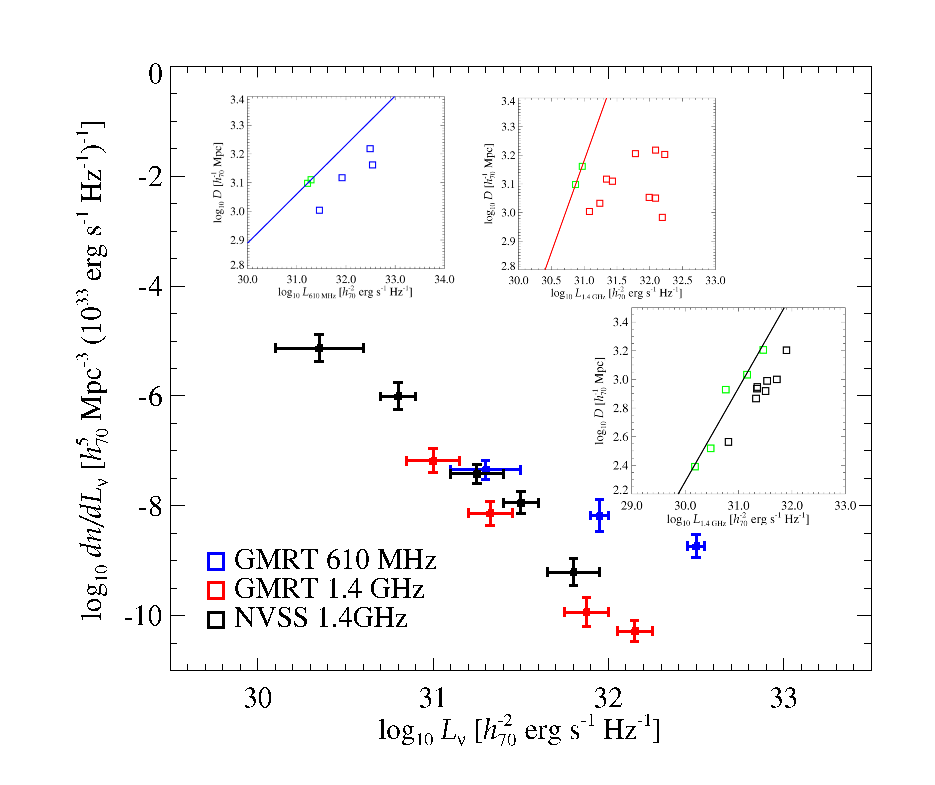
\includegraphics[width=0.48\textwidth]{figures/RLF_observations.eps}
\caption{Radio luminosity function obtained from existent observations. The three insets show the luminosity-distance distribution of the three samples (see main text for details) where the solid line is the fit to the upper envelope population, indicated in green, employed to calculate the flux limit for the classical $V_{max}$ estimator. The choice of the upper envelope population is somehow arbitrary, particularly in the GMRT cases due to the unhappy luminosity--distance distributions. The horizontal error bars represent the mass bins while the vertical error bars are Poissonian uncertainties.}
\label{fig:RLFobs}
\end{figure}

\end{appendix}

%%%%%%%%%%%%%%%%%%%%%%%%%%%%%%%%%%%%%%%%%%%%%%%%%%%%%%%%%%%%%%%%%%%
%%%%%%%%%%%%%%%%%%%%%%%%%%%%%%%%%%%%%%%%%%%%%%%%%%%%%%%%%%%%%%%%%%%
\bibliographystyle{aa}
\bibliography{bib_file}


%%%%%%%%%%%%%%%%%%%%%%%%%%%%%%%%%%%%%%%%%%%%%%%%%%%%%%%%%%%%%%%%%%
%%%%%%%%%%%%%%%%%%%%%%%%%%%%%%%%%%%%%%%%%%%%%%%%%%%%%%%%%%%%%%%%%%
\end{document}

